\documentclass[12pt,a4paper]{article}
%DIF LATEXDIFF DIFFERENCE FILE
%DIF DEL C:\Users\nicol\Desktop\LIFE\LIFESim\thesis\.diff_tmp\main_old.tex   Fri Jul 24 17:58:16 2026
%DIF ADD C:\Users\nicol\Desktop\LIFE\LIFESim\thesis\.diff_tmp\main_new.tex   Fri Jul 24 17:58:16 2026
%DIF 2a2
\usepackage{fix-cm} %DIF > 
%DIF -------
\usepackage{setspace}
\usepackage{fancyhdr}
\usepackage{lettrine}
\usepackage{geometry}
\usepackage[english]{babel}
\usepackage[utf8]{inputenc}
\usepackage{dcolumn}
\usepackage{array,booktabs,ragged2e}
\usepackage{pgfplots,pgfplotstable,pgfkeys,filecontents}
\usepackage{csvsimple,ifthen,etoolbox}
\usepackage{amsmath,latexsym}
\usepackage{gensymb}
\usepackage{amssymb}
\usepackage{amsmath}
\usepackage{tikz}
\usepackage{xfrac}
\usepackage{fancyhdr}
\usepackage{lettrine}
\usepackage{geometry}
\usepackage{dcolumn}
\usepackage[htt]{hyphenat}
\usepackage{circuitikz}
\usepackage{siunitx}
\usepackage{nicefrac}
\usepackage{hyperref}
%DIF 27a28
\usepackage{xurl} %DIF > 
%DIF -------
\usepackage{color,soul}
\usepackage{titlesec}
\usepackage[T1]{fontenc}
\usepackage{adjustbox}
\usepackage{pdfpages}
\usepackage{multirow}
\usepackage{graphicx}
\usepackage{wrapfig}
\usetikzlibrary{fit}
\usepackage{float}
\usepackage{rotating}
%DIF 38a40
\usepackage{pdflscape} %DIF > 
%DIF -------
\usepackage{caption}
\usepackage{subcaption}
\usepackage{mathtools}
\usepackage{upgreek}
\usepackage[toc,page]{appendix}
\usepackage[section]{placeins}

% --- Float placement: keep figures near their references ---
\setcounter{topnumber}{4}
\setcounter{bottomnumber}{4}
\setcounter{totalnumber}{6}
\renewcommand{\topfraction}{0.9}
\renewcommand{\bottomfraction}{0.9}
\renewcommand{\textfraction}{0.05}
\renewcommand{\floatpagefraction}{0.8}

\newcommand\addvmargin[1]{
	\node[fit=(current bounding box),inner ysep=#1,inner xsep=0]{};
}
\geometry{
	a4paper,
	total={8.5in,11in},
	left=1in,
	right=1in,
	top=1in,
	bottom=1in,
}

\pagestyle{fancy}
%DIF 67a70
\setlength{\headheight}{28pt} %DIF > 
%DIF -------

\raggedbottom
\newcolumntype{R}[1]{>{\RaggedLeft\arraybackslash}p{#1}}
\renewcommand{\baselinestretch}{1.4}
\setlength\parindent{0pt}
\def\doubleunderline#1{\underline{\underline{#1}}}

\newcommand{\reporttitle}[3][ ]{
	\thispagestyle{empty}
	\begin{center}
		\vspace*{8mm}
		\fontshape{sc}
		\fontsize{17pt}{20pt}
		\selectfont
		#2
		\linebreak
		\fontsize{25pt}{25pt}
		\bfseries
		\selectfont
		#3
		\linebreak
		\fontshape{n}
		\fontsize{15pt}{25pt}
		\normalfont
		\selectfont
		#1
	\end{center}
}

% Header ============================================================================================
\pagestyle{fancy}
\fancyhf{}
%DIF 99c103
%DIF < \lhead{Master's Thesis - 1st Draft\\IPA / Quanz Group}
%DIF -------
\lhead{Master's Thesis\\IPA / Quanz Group} %DIF > 
%DIF -------
\renewcommand{\sectionmark}[1]{\markboth{#1}{}}
%DIF 101c105
%DIF < \chead{DATE\\ \nouppercase{\leftmark}}
%DIF -------
\chead{July 2026\\ \nouppercase{\leftmark}} %DIF > 
%DIF -------
\rhead{FS 26\\Nicolas Feuchthofen}
\cfoot{Page \thepage}
%DIF 104a108-157
 %DIF > 
\fancypagestyle{chapteropening}{ %DIF > 
    \fancyhf{} %DIF > 
    \cfoot{Page \thepage} %DIF > 
    \renewcommand{\headrulewidth}{0pt} %DIF > 
} %DIF > 
 %DIF > 
\definecolor{lifeaccent}{HTML}{76232F} %DIF > 
\definecolor{lifepale}{HTML}{E9E4E5} %DIF > 
\definecolor{lifegray}{HTML}{727272} %DIF > 
 %DIF > 
\newif\ifappendixchapter %DIF > 
\appendixchapterfalse %DIF > 
 %DIF > 
\newcommand{\chapteropening}[2]{% %DIF > 
    \clearpage %DIF > 
    \refstepcounter{section}% %DIF > 
    \sectionmark{#1}% %DIF > 
    \addcontentsline{toc}{section}{\protect\numberline{\thesection}#1}% %DIF > 
    \thispagestyle{chapteropening}% %DIF > 
    \begin{tikzpicture}[remember picture,overlay] %DIF > 
        \fill[lifeaccent] %DIF > 
            ([xshift=24mm,yshift=-28mm]current page.north west) %DIF > 
            rectangle %DIF > 
            ([xshift=28mm,yshift=-105mm]current page.north west); %DIF > 
        \node[ %DIF > 
            anchor=base east, %DIF > 
            text=lifepale, %DIF > 
            font=\fontsize{72}{72}\selectfont\bfseries %DIF > 
        ] at ([xshift=-20mm,yshift=-35mm]current page.north east) {\thesection}; %DIF > 
    \end{tikzpicture}% %DIF > 
    \vspace*{26mm} %DIF > 
    \hspace*{13mm}% %DIF > 
    \begin{minipage}{0.82\textwidth} %DIF > 
        {\color{lifeaccent}\fontsize{10}{12}\selectfont\bfseries\scshape %DIF > 
        \ifappendixchapter Appendix\else Chapter\fi~\thesection} %DIF > 
 %DIF > 
        \vspace{7mm} %DIF > 
 %DIF > 
        {\hyphenpenalty=10000\exhyphenpenalty=10000 %DIF > 
        \RaggedRight\fontsize{32}{36}\selectfont\bfseries #1\par} %DIF > 
 %DIF > 
        \vspace{7mm} %DIF > 
 %DIF > 
        {\color{lifegray}\RaggedRight\large #2\par} %DIF > 
    \end{minipage}\par %DIF > 
 %DIF > 
    \vspace{28mm} %DIF > 
    \noindent\ignorespaces %DIF > 
} %DIF > 
%DIF -------

%\setlength{\columnsep}{5mm}
%\setlength{\columnseprule}{0.5pt}
\setlength{\parindent}{0pt}
\renewcommand{\baselinestretch}{1.4}
\setlength{\parskip}{3mm}
% ===============================================================================================================

\onehalfspacing

\numberwithin{equation}{section}
\numberwithin{figure}{section}
\numberwithin{table}{section}
%DIF PREAMBLE EXTENSION ADDED BY LATEXDIFF
%DIF UNDERLINE PREAMBLE %DIF PREAMBLE
\RequirePackage[normalem]{ulem} %DIF PREAMBLE
\RequirePackage{color}\definecolor{RED}{rgb}{1,0,0}\definecolor{BLUE}{rgb}{0,0,1} %DIF PREAMBLE
\providecommand{\DIFaddtex}[1]{{\protect\color{blue}\uwave{#1}}} %DIF PREAMBLE
\providecommand{\DIFdeltex}[1]{{\protect\color{red}\sout{#1}}} %DIF PREAMBLE
%DIF SAFE PREAMBLE %DIF PREAMBLE
\providecommand{\DIFaddbegin}{} %DIF PREAMBLE
\providecommand{\DIFaddend}{} %DIF PREAMBLE
\providecommand{\DIFdelbegin}{} %DIF PREAMBLE
\providecommand{\DIFdelend}{} %DIF PREAMBLE
\providecommand{\DIFmodbegin}{} %DIF PREAMBLE
\providecommand{\DIFmodend}{} %DIF PREAMBLE
%DIF FLOATSAFE PREAMBLE %DIF PREAMBLE
\providecommand{\DIFaddFL}[1]{\DIFadd{#1}} %DIF PREAMBLE
\providecommand{\DIFdelFL}[1]{\DIFdel{#1}} %DIF PREAMBLE
\providecommand{\DIFaddbeginFL}{} %DIF PREAMBLE
\providecommand{\DIFaddendFL}{} %DIF PREAMBLE
\providecommand{\DIFdelbeginFL}{} %DIF PREAMBLE
\providecommand{\DIFdelendFL}{} %DIF PREAMBLE
%DIF HYPERREF PREAMBLE %DIF PREAMBLE
\providecommand{\DIFadd}[1]{\texorpdfstring{\DIFaddtex{#1}}{#1}} %DIF PREAMBLE
\providecommand{\DIFdel}[1]{\texorpdfstring{\DIFdeltex{#1}}{}} %DIF PREAMBLE
\newcommand{\DIFscaledelfig}{0.5}
%DIF HIGHLIGHTGRAPHICS PREAMBLE %DIF PREAMBLE
\RequirePackage{settobox} %DIF PREAMBLE
\RequirePackage{letltxmacro} %DIF PREAMBLE
\newsavebox{\DIFdelgraphicsbox} %DIF PREAMBLE
\newlength{\DIFdelgraphicswidth} %DIF PREAMBLE
\newlength{\DIFdelgraphicsheight} %DIF PREAMBLE
% store original definition of \includegraphics %DIF PREAMBLE
\LetLtxMacro{\DIFOincludegraphics}{\includegraphics} %DIF PREAMBLE
\newcommand{\DIFaddincludegraphics}[2][]{{\color{blue}\fbox{\DIFOincludegraphics[#1]{#2}}}} %DIF PREAMBLE
\newcommand{\DIFdelincludegraphics}[2][]{% %DIF PREAMBLE
\sbox{\DIFdelgraphicsbox}{\DIFOincludegraphics[#1]{#2}}% %DIF PREAMBLE
\settoboxwidth{\DIFdelgraphicswidth}{\DIFdelgraphicsbox} %DIF PREAMBLE
\settoboxtotalheight{\DIFdelgraphicsheight}{\DIFdelgraphicsbox} %DIF PREAMBLE
\scalebox{\DIFscaledelfig}{% %DIF PREAMBLE
\parbox[b]{\DIFdelgraphicswidth}{\usebox{\DIFdelgraphicsbox}\\[-\baselineskip] \rule{\DIFdelgraphicswidth}{0em}}\llap{\resizebox{\DIFdelgraphicswidth}{\DIFdelgraphicsheight}{% %DIF PREAMBLE
\setlength{\unitlength}{\DIFdelgraphicswidth}% %DIF PREAMBLE
\begin{picture}(1,1)% %DIF PREAMBLE
\thicklines\linethickness{2pt} %DIF PREAMBLE
{\color[rgb]{1,0,0}\put(0,0){\framebox(1,1){}}}% %DIF PREAMBLE
{\color[rgb]{1,0,0}\put(0,0){\line( 1,1){1}}}% %DIF PREAMBLE
{\color[rgb]{1,0,0}\put(0,1){\line(1,-1){1}}}% %DIF PREAMBLE
\end{picture}% %DIF PREAMBLE
}\hspace*{3pt}}} %DIF PREAMBLE
} %DIF PREAMBLE
\LetLtxMacro{\DIFOaddbegin}{\DIFaddbegin} %DIF PREAMBLE
\LetLtxMacro{\DIFOaddend}{\DIFaddend} %DIF PREAMBLE
\LetLtxMacro{\DIFOdelbegin}{\DIFdelbegin} %DIF PREAMBLE
\LetLtxMacro{\DIFOdelend}{\DIFdelend} %DIF PREAMBLE
\DeclareRobustCommand{\DIFaddbegin}{\DIFOaddbegin \let\includegraphics\DIFaddincludegraphics} %DIF PREAMBLE
\DeclareRobustCommand{\DIFaddend}{\DIFOaddend \let\includegraphics\DIFOincludegraphics} %DIF PREAMBLE
\DeclareRobustCommand{\DIFdelbegin}{\DIFOdelbegin \let\includegraphics\DIFdelincludegraphics} %DIF PREAMBLE
\DeclareRobustCommand{\DIFdelend}{\DIFOaddend \let\includegraphics\DIFOincludegraphics} %DIF PREAMBLE
\LetLtxMacro{\DIFOaddbeginFL}{\DIFaddbeginFL} %DIF PREAMBLE
\LetLtxMacro{\DIFOaddendFL}{\DIFaddendFL} %DIF PREAMBLE
\LetLtxMacro{\DIFOdelbeginFL}{\DIFdelbeginFL} %DIF PREAMBLE
\LetLtxMacro{\DIFOdelendFL}{\DIFdelendFL} %DIF PREAMBLE
\DeclareRobustCommand{\DIFaddbeginFL}{\DIFOaddbeginFL \let\includegraphics\DIFaddincludegraphics} %DIF PREAMBLE
\DeclareRobustCommand{\DIFaddendFL}{\DIFOaddendFL \let\includegraphics\DIFOincludegraphics} %DIF PREAMBLE
\DeclareRobustCommand{\DIFdelbeginFL}{\DIFOdelbeginFL \let\includegraphics\DIFdelincludegraphics} %DIF PREAMBLE
\DeclareRobustCommand{\DIFdelendFL}{\DIFOaddendFL \let\includegraphics\DIFOincludegraphics} %DIF PREAMBLE
%DIF AMSMATHULEM PREAMBLE %DIF PREAMBLE
\makeatletter %DIF PREAMBLE
\let\sout@orig\sout %DIF PREAMBLE
\renewcommand{\sout}[1]{\ifmmode\text{\sout@orig{\ensuremath{#1}}}\else\sout@orig{#1}\fi} %DIF PREAMBLE
\makeatother %DIF PREAMBLE
%DIF COLORLISTINGS PREAMBLE %DIF PREAMBLE
\RequirePackage{listings} %DIF PREAMBLE
\RequirePackage{color} %DIF PREAMBLE
\lstdefinelanguage{DIFcode}{ %DIF PREAMBLE
%DIF DIFCODE_UNDERLINE %DIF PREAMBLE
  moredelim=[il][\color{red}\sout]{\%DIF\ <\ }, %DIF PREAMBLE
  moredelim=[il][\color{blue}\uwave]{\%DIF\ >\ } %DIF PREAMBLE
} %DIF PREAMBLE
\lstdefinestyle{DIFverbatimstyle}{ %DIF PREAMBLE
	language=DIFcode, %DIF PREAMBLE
	basicstyle=\ttfamily, %DIF PREAMBLE
	columns=fullflexible, %DIF PREAMBLE
	keepspaces=true %DIF PREAMBLE
} %DIF PREAMBLE
\lstnewenvironment{DIFverbatim}{\lstset{style=DIFverbatimstyle}}{} %DIF PREAMBLE
\lstnewenvironment{DIFverbatim*}{\lstset{style=DIFverbatimstyle,showspaces=true}}{} %DIF PREAMBLE
\lstset{extendedchars=\true,inputencoding=utf8}

%DIF END PREAMBLE EXTENSION ADDED BY LATEXDIFF

\begin{document}
% Compatibility labels for references deleted in the new revision.
\phantomsection\label{eq: additive noise}
\phantomsection\label{fig: astronoise}
\phantomsection\label{fig: image size convergence}
\phantomsection\label{fig: image size convergence a}
\phantomsection\label{fig: image size convergence b}
\phantomsection\label{fig: leakage budget example}
\phantomsection\label{fig: spec res convergence}
\phantomsection\label{fig: tse budget hab2min}
\phantomsection\label{fig: tse budget shapes}
\phantomsection\label{fig: tse budget shapes a}
\phantomsection\label{fig: tse budget shapes b}
\phantomsection\label{fig: tse budget shapes c}
\phantomsection\label{fig: tse iso magfor a}
\phantomsection\label{fig: tse iso magfor b}
\phantomsection\label{fig: tse iso slewfor a}
\phantomsection\label{fig: tse iso slewfor b}
\phantomsection\label{fig: tse linear additive a}
\phantomsection\label{fig: tse linear additive b}
\phantomsection\label{tab: budget result}
% Titel ========================================================================================================
\DIFdelbegin %DIFDELCMD < \reporttitle[\vspace{-1.5cm} \\ \rule{6.4cm}{0.4pt} \\ \vspace{-0.5cm} \textit{Nicolas Feuchthofen} \\ Supervisors: Dr. Felix Dannert, Prof. Dr. Sascha Patrick Quanz\\ \vspace{-0.4cm}  DATE]{Master's Thesis - 1st Draft}{Finding Optimal Random Noise Error Budget Distributions for the LIFE Space Mission With Arbitrary Nulling and Noise Models}
%DIFDELCMD < %%%
\DIFdelend \DIFaddbegin \reporttitle[\vspace{-1.5cm} \\ \rule{6.4cm}{0.4pt} \\ \vspace{-0.5cm} \textit{Nicolas Feuchthofen} \\ Supervisors: Dr. Felix Dannert, Prof. Dr. Sascha Patrick Quanz\\ \vspace{-0.4cm} July 2026]{Master's Thesis}{Instrument-Agnostic Iso-Mission-Time Noise Budgets for LIFE Using a Null-Order Proxy}
\DIFaddend 

\vspace{1cm}

\begin{figure}[htp]
    \centering
    
\includegraphics[width=0.5\linewidth]{images/LIFE_Logo_Wordmark_Primary_Digital_RBG-Black.png}
\end{figure}

\vspace{1cm}

\DIFdelbegin %DIFDELCMD < \begin{abstract}
%DIFDELCMD <     %%%
\DIFdel{TODO
}%DIFDELCMD < \end{abstract}
%DIFDELCMD < 

%DIFDELCMD < %%%
\DIFdelend \newpage

%DIF <  ===============================================================================================================
\DIFaddbegin \begin{abstract}
    \DIFadd{The Large Interferometer For Exoplanets (LIFE) aims to detect and characterize nearby terrestrial exoplanets in the mid-infrared. Its scientific return depends on how much additional instrumental random noise can be tolerated without making the required observing program too long. This thesis develops an Agnostic Mission Simulator (AMS) and a trade-space explorer that convert a wavelength-dependent aggregate random-noise allowance into a 90th-percentile mission time. The source calculation was reformulated analytically for circularly symmetric astrophysical backgrounds, eliminating the former spatial pixel grid, correcting the local-zodiacal normalization by about 27\%, and permitting accurate wavelength-bin quadrature. The AMS reproduces the shared LIFEsim source-model SNRs to floating-point precision.
}\DIFaddend 

    \DIFdelbegin \section*{\DIFdel{Acknowledgments}}
%DIFAUXCMD
\DIFdel{TODO
}\DIFdelend \DIFaddbegin \DIFadd{Final calculations compare three additive budget shapes---flat, short-weighted, and long-weighted---for the Hab2Max and Hab2Min catalogs at limiting magnitude 7, field of regard $65^\circ$, and 12\,h slew time. For the second-order double-Bracewell reference, the short-weighted ramp admits the largest endpoint, consistent with geometric stellar leakage dominating the short-wavelength variance. In the fourth-order proxy, stellar leakage is suppressed by three to five orders of magnitude and the ordering reverses: zodiacal backgrounds dominate and the long-weighted ramp admits the largest endpoint. At the primary mission-time targets, the flat allowance rises from 140 to 650\,ph\,s$^{-1}$\,$\upmu$m$^{-1}$ for Hab2Max at 5.5\,yr and from 65 to 590\,ph\,s$^{-1}$\,$\upmu$m$^{-1}$ for Hab2Min at 7.5\,yr when changing from null order two to four.
}\DIFaddend 

    \DIFaddbegin \DIFadd{These values are iso-mission-time amplitudes within tested budget families, not wavelength-by-wavelength subsystem requirements. The null-order comparison uses an unnormalized $\sin^n$ transmission proxy with fixed collecting area, efficiency, and baseline prescription; it therefore measures the impact of the modeled null order and its associated throughput change rather than predicting a concrete fourth-order LIFE architecture.
}\end{abstract}

\DIFaddend \newpage

% ===============================================================================================================

\tableofcontents

\DIFdelbegin %DIFDELCMD < \newpage
%DIFDELCMD < %%%
\DIFdelend \DIFaddbegin \chapteropening{Introduction}{Why LIFE matters and how a science goal becomes an instrument requirement}
\DIFadd{Human curiosity extends far beyond Earth. We seek to understand how life began and whether Earth is its only home in the Galaxy. The Large Interferometer For Exoplanets (LIFE) turns that broad question into a concrete observational program: detecting nearby temperate terrestrial planets in the mid-infrared, measuring their thermal spectra, and using those measurements to constrain planet populations, atmospheric composition, and possible habitability \mbox{%DIFAUXCMD
\cite{quanz2022life1,konrad2022life3}}\hskip0pt%DIFAUXCMD
.
}\DIFaddend 

\DIFdelbegin \section{\DIFdel{Introduction}}
%DIFAUXCMD
\addtocounter{section}{-1}%DIFAUXCMD
\DIFdel{At the moment, the error budget , which is the maximum allowed total noise, of the LIFE space mission is estimated using a double Bracewell interferometer architecture. Currently, astrophysical noise sources are computed from known models.
The required mission time is then usually derived without instrumental noise, or using arbitrary additional instrumental noise terms. This approach is very simple and understandable, but unfortunately it does not completely meet the complex requirements of the mission.
}\DIFdelend \DIFaddbegin \DIFadd{For me, this scientific promise makes the practical definition of LIFE especially consequential. A mission can deliver those measurements only if its instrument can be built and operated within credible performance limits. This project therefore asks how much aggregate instrumental random noise LIFE can tolerate, and where in wavelength that noise is least damaging, before the required observing program becomes too long. Answering that question helps define instrument boundaries, test the feasibility of the approach, and increase confidence in both the mission concept and the conclusions drawn from its measurements.
}\DIFaddend 

\DIFdelbegin \DIFdel{First, there is no study on the impact of varying noise on mission time. We simply do not know the optimal budget assignment at the moment. In instrument engineering, not all noise sources are equally easily optimizable. We must hence be able to include not only the absolute value, but also the distribution of the error budget in sensible instrument requirement calculations.
Second, there lies a fundamental problem in the assumption of an instrument architecture. How do we know whether the double Bracewell is actually ideal for our mission? There might be a different nulling architecture that is simpler to construct and control while actually completing the mission in less time}\DIFdelend \DIFaddbegin \DIFadd{The reference LIFE studies used here establish the astrophysical source model, signal extraction, and expected detection and characterization performance for a double-Bracewell interferometer \mbox{%DIFAUXCMD
\cite{quanz2022life1,dannert2022life2,dannert2025thesis}}\hskip0pt%DIFAUXCMD
. They do not yet provide the wavelength-dependent iso-mission-time boundary for a mechanism-independent aggregate random-noise term. This thesis fills that narrower gap with two linked tools. The }\textit{\DIFadd{Agnostic Mission Simulator}} \DIFadd{(AMS) maps a specified noise budget and operating point to mission time; the }\textit{\DIFadd{Trade Space Explorer}} \DIFadd{(TSE) inverts that mapping to find the largest tolerated budget amplitude. A controlled change from a second- to a fourth-order transmission proxy then reveals an initially counter-intuitive reversal: the spectral region that tolerates the most added noise changes when geometric stellar leakage is strongly suppressed}\DIFaddend .

\DIFdelbegin \DIFdel{To summarize, we currently know neither which instrument architecture is the best for our case nor how accurately we must engineer that architecture to be able to achieve the scientific goals in a realistic time.
}\DIFdelend \DIFaddbegin \DIFadd{This work keeps the double Bracewell as its reference geometry. It is mechanism-agnostic only for an aggregate random-noise allowance: individual independent random terms are represented by their common equivalent rate. The result is therefore a bridge quantity. It translates a science-level completion time into an allowed single-output random count rate at a defined pre-efficiency reference plane. A later engineering allocation can map detector, optical, thermal, and control-noise terms to that plane and test their combined variance against the allowance. This thesis does not perform that subsystem allocation and cannot decide which hardware implementation is easiest. Architecture dependence is parameterized only through the explicitly limited null-order proxy, not through an arbitrary-architecture simulation.
}\DIFaddend 

\DIFdelbegin \DIFdel{In order to find an answer to both very pressing questions, we propose a different approach. Instead of assuming a fixed instrument and simulating noise based on it, we use noise and planet signals as input. These inputs must conform to the astrophysical limit. By changing the inputs and their functional forms, we also challenge the instrument architecture since it is fundamentally connected to signal and noise through interferometry physics. This approach does not rely on any assumptions on architecture, works with any order nulling, and is therefore }\textit{\DIFdel{instrument-agnostic}}%DIFAUXCMD
\DIFdel{. }%DIFDELCMD < 

%DIFDELCMD < %%%
\DIFdelend \subsection{Research Questions} \label{sec: intro: research questions}
\DIFdelbegin \DIFdel{Using a set of novel approaches, this thesis project will seek to answer }\DIFdelend \DIFaddbegin \DIFadd{This thesis addresses }\DIFaddend the following central question.

\textit{\DIFdelbegin \DIFdel{Using an efficient architecture-agnostic simulator for arbitrary physics-conforming nulling }\DIFdelend \DIFaddbegin \DIFadd{For a specified operating point }\DIFaddend and \DIFdelbegin \DIFdel{noise models, can we reliably determine instrument-agnostic requirements on the overall random noise error budget of the LIFE space mission to complete the mission in }\DIFdelend a \DIFdelbegin \DIFdel{reasonable amount }\DIFdelend \DIFaddbegin \DIFadd{tested family }\DIFaddend of \DIFdelbegin \DIFdel{time}\DIFdelend \DIFaddbegin \DIFadd{additive random-noise budgets}\DIFaddend , \DIFdelbegin \DIFdel{assuming pessimistic constraints on the physical limits}\DIFdelend \DIFaddbegin \DIFadd{what maximum budget amplitude is compatible with completing Experiment~1---the inherited detection-and-characterization program for 50 qualifying catalog planets---within a chosen mission-time target}\DIFaddend ?}

This question \DIFdelbegin \DIFdel{may be }\DIFdelend \DIFaddbegin \DIFadd{is }\DIFaddend structured into the following sub-questions\DIFdelbegin \DIFdel{, which the thesis will address in detail}\DIFdelend :
\begin{itemize}
    \item \textit{What is the dimension of the AMS parameter space?}
    \item \DIFaddbegin \textit{\DIFadd{Which source-model computations can be reused when only global filters or tested budget amplitudes change?}}
    \item \DIFaddend \textit{Can we reduce the AMS parameter space without significantly compromising fidelity?}
    \item \textit{Can we \DIFdelbegin \DIFdel{determine a set of optimal, i. e. architecturally most easily feasible, parameters }\DIFdelend \DIFaddbegin \DIFadd{locate the maximum tolerated amplitude }\DIFaddend for \DIFdelbegin \DIFdel{any set mission time, assuming any realizable nulling architecture}\DIFdelend \DIFaddbegin \DIFadd{flat and linear-ramp random-noise budgets at a fixed operating point}\DIFaddend ?}
    \item \textit{\DIFdelbegin \DIFdel{Can we efficiently and deeply explore }\DIFdelend \DIFaddbegin \DIFadd{How does changing }\DIFaddend the \DIFdelbegin \DIFdel{parameter space of }\DIFdelend \DIFaddbegin \DIFadd{null order represented by }\DIFaddend the \DIFdelbegin \DIFdel{AMS to be able to provide a solution that is as close to optimal as possible}\DIFdelend \DIFaddbegin \DIFadd{transmission proxy alter the tolerated spectral budget shapes}\DIFaddend ?}
\end{itemize}

The remainder \DIFdelbegin \DIFdel{of this thesis follows the logic of these questions}\DIFdelend \DIFaddbegin \DIFadd{follows the causal chain from mission goal to engineering requirement}\DIFaddend . Section \ref{sec: background} \DIFdelbegin \DIFdel{lays out the theory needed to follow the approach: the target catalogs, the signal-to-noise ratio, the noise sources, and the notion of an error budgetspread over a large trade space}\DIFdelend \DIFaddbegin \DIFadd{establishes the experiment, target populations, measurement, SNR, and error budget}\DIFaddend . Section \ref{sec: methods} \DIFdelbegin \DIFdel{then constructs the instrument-agnostic machinery itself, the functional treatment of the variable parameters, the modified null-depth ansatz that stands in for the architecture, and the Agnostic Mission Simulator that turns a set of parameters into a mission time}\DIFdelend \DIFaddbegin \DIFadd{builds the fixed-reference simulator and null-order proxy}\DIFaddend . Section \ref{sec: ts reduction} \DIFdelbegin \DIFdel{attacks the first two sub-questions by shrinking the trade space without sacrificing fidelity, and Section \ref{sec: tse} explores the reduced space to answer the remaining two. We close with a discussion of what the approach achieves and where it can still be improved}\DIFdelend \DIFaddbegin \DIFadd{reduces the raw trade space and derives the analytic background response. Section \ref{sec: tse} then presents the completed exploration, first at the nominal second-order null and then at fourth order. The discussion and conclusion state what the resulting allowances do and do not imply for LIFE}\DIFaddend .

\DIFdelbegin %DIFDELCMD < \newpage
%DIFDELCMD < %%%
\section{\DIFdel{Background and Procedures}} %DIFAUXCMD
\addtocounter{section}{-1}%DIFAUXCMD
\DIFdelend \DIFaddbegin \chapteropening{Background and Procedures}{From a synthetic planetary population to a measurable mission signal} \DIFaddend \label{sec: background}
This project is \DIFdelbegin \DIFdel{being }\DIFdelend conducted within the scope of the LIFE space mission. \DIFdelbegin \DIFdel{The mission aims to use nulling interferometry to block most of the light of individual stars to be able to detect the thermal emissions of orbiting exoplanets. This will be achieved by placing a rotating array of apertures at the Sun-Earth L2 Lagrange point. By flying in formation, the collected light may be combined to form a large }\DIFdelend \DIFaddbegin \DIFadd{To connect its scientific objective to an engineering requirement, we first need to establish what the experiment asks the instrument to observe and how those observations become a mission-time calculation. LIFE is a proposed space-based }\DIFaddend mid-infrared \DIFdelbegin \DIFdel{interferometer. The presence of different molecular species, including potential biomarkers, can be indicated by the absorption features in the retrieved spectra, providing clues to the existence of extraterrestrial life. We currently work with a double Bracewell mission architecture, which is made up of two pairs of apertures, producing two dark (destructive interference) and two bright (constructive interference) outputswith a null order of two , as depicted in Fig. \ref{fig: double-bracewell-layout}. This chapter defines the background and theory necessary to be able to follow our approach.
}\DIFdelend \DIFaddbegin \DIFadd{nulling interferometer for detecting and characterizing nearby temperate terrestrial planets \mbox{%DIFAUXCMD
\cite{quanz2022life1,dannert2022life2}}\hskip0pt%DIFAUXCMD
. Its current concept separates light collection from beam combination: four free-flying collector spacecraft feed a central beam-combiner spacecraft while the formation rotates about the line of sight. The long effective baseline supplies angular resolution that a single space telescope of comparable total collecting area could not provide.
}\DIFaddend 

\DIFaddbegin \DIFadd{The scientific reason for observing in the mid-infrared is twofold. A temperate planet emits much of its thermal radiation in this range, reducing the star--planet contrast relative to visible reflected light, and several atmospheric molecules have diagnostically useful absorption bands there. Nulling interferometry does not form a conventional resolved image of every system. Instead, it suppresses the on-axis star, modulates off-axis emission through rotation, and measures a wavelength-dependent differential signal. Detecting that signal constrains planet populations; accumulating a spectrum can constrain atmospheric composition. The latter remains an inference problem rather than an automatic identification of life \mbox{%DIFAUXCMD
\cite{quanz2022life1,konrad2022life3}}\hskip0pt%DIFAUXCMD
.
}

\DIFadd{This thesis retains the four-aperture double-Bracewell response used by LIFEsim \mbox{%DIFAUXCMD
\cite{dannert2022life2}}\hskip0pt%DIFAUXCMD
. Two aperture pairs first produce destructive and constructive outputs. The destructive outputs are recombined with a relative phase shift to produce two chopped dark outputs whose difference changes sign for an off-axis source. The reference response has a second-order intensity null: close to the optical axis, transmitted stellar intensity grows quadratically with angular offset. Figure \ref{fig: double-bracewell-layout} shows this optical logic.
}

\DIFaddend \begin{figure}[htbp]
    \centering
    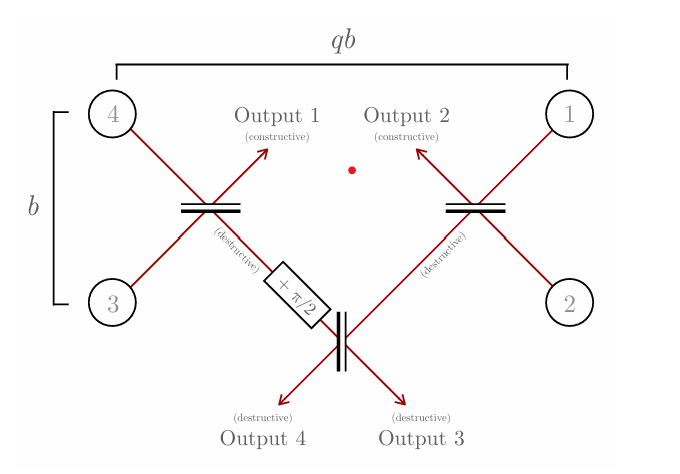
\includegraphics[width=0.8\linewidth]{images/intro/dannert2022-double-bracewell-layout.png}
    \caption{\DIFaddbeginFL \DIFaddFL{Double-Bracewell interferometer layout reproduced from }\DIFaddendFL Dannert et al. \DIFdelbeginFL \DIFdelFL{(2022): Double Bracewell interferometer layout for the LIFE space mission}\DIFdelendFL \DIFaddbeginFL \DIFaddFL{\mbox{%DIFAUXCMD
\cite{dannert2022life2}}\hskip0pt%DIFAUXCMD
}\DIFaddendFL . Light from apertures 4 and 3, \DIFaddbeginFL \DIFaddFL{and from }\DIFaddendFL 1 and 2\DIFaddbeginFL \DIFaddFL{, }\DIFaddendFL is combined to form \DIFdelbeginFL \DIFdelFL{two }\DIFdelendFL destructive and \DIFdelbeginFL \DIFdelFL{two }\DIFdelendFL constructive outputs. The destructive outputs are \DIFdelbeginFL \DIFdelFL{combined again }\DIFdelendFL \DIFaddbeginFL \DIFaddFL{recombined }\DIFaddendFL with a \DIFaddbeginFL \DIFaddFL{relative }\DIFaddendFL phase shift of $\pi/2$ to form \DIFdelbeginFL \DIFdelFL{the }\DIFdelendFL two \DIFaddbeginFL \DIFaddFL{chopped }\DIFaddendFL dark outputs with a \DIFdelbeginFL \DIFdelFL{second order }\DIFdelendFL \DIFaddbeginFL \DIFaddFL{second-order }\DIFaddendFL null.}
    \label{fig: double-bracewell-layout}
\end{figure}

\newpage

\subsection{The Experiment and Assumptions}
This work \DIFdelbegin \DIFdel{focuses on }\DIFdelend \DIFaddbegin \DIFadd{adopts the legacy LIFEsim/AMS configuration called }\DIFaddend \textit{Experiment 1}\DIFdelbegin \DIFdel{of the LIFE mission , a sub-mission aiming to }\DIFdelend \DIFaddbegin \DIFadd{: the mission must }\DIFaddend detect and characterize \DIFdelbegin \DIFdel{at least }\DIFdelend 50 \DIFdelbegin \DIFdel{terrestrial planets }\DIFdelend \DIFaddbegin \DIFadd{catalog planets with radii }\DIFaddend between 0.5 and 1.5 Earth radii\DIFdelbegin \DIFdel{in the habitable zone of sun-like stars (stellar temperature }\DIFdelend \DIFaddbegin \DIFadd{, host-star temperatures }\DIFaddend between 4370 \DIFdelbegin \DIFdel{K }\DIFdelend and 7310\DIFaddbegin \DIFadd{\,K, and a positive catalog habitable-zone flag. The thresholds and instrument settings used throughout the completed data collection are summarized in Table \ref{tab: study assumptions}. They define this study's controlled comparison; they should not be read as a claim that every value is the latest top-level LIFE mission requirement.
}

\begin{table}[htbp]
\centering
\begin{tabular}{@{}p{0.35\linewidth}p{0.21\linewidth}p{0.34\linewidth}@{}}
\toprule
\DIFaddFL{Quantity }& \DIFaddFL{Adopted value }& \DIFaddFL{Role in the calculation }\\
\midrule
\DIFaddFL{Qualifying sample }& \DIFaddFL{50 planets }& \DIFaddFL{Experiment-completion target }\\
\DIFaddFL{Planet radius }& \DIFaddFL{$0.5$--$1.5\,R_\oplus$ }& \DIFaddFL{Catalog eligibility filter }\\
\DIFaddFL{Host temperature }& \DIFaddFL{4370--7310\,}\DIFaddendFL K \DIFdelbeginFL \DIFdelFL{) (CITATION). For a successful characterization , we assume a minimum signal-to-noise-ratio of 44. Each aperture is optimistically assumed to possess a fixed mirror size of }\DIFdelendFL \DIFaddbeginFL & \DIFaddFL{Catalog eligibility filter }\\
\DIFaddFL{Habitable zone }& \DIFaddFL{Catalog flag required }& \DIFaddFL{Catalog eligibility filter }\\
\DIFaddFL{Detection threshold }& \DIFaddFL{SNR 7 }& \DIFaddFL{Common detection campaign }\\
\DIFaddFL{Characterization threshold }& \DIFaddFL{SNR 44.1 }& \DIFaddFL{Broadband characterization proxy }\\
\DIFaddFL{Orbit epochs }& \DIFaddFL{5 }& \DIFaddFL{Detection plus four follow-up visits }\\
\DIFaddFL{Collector diameter }& \DIFaddendFL 4\DIFaddbeginFL \DIFaddFL{\,m each }& \DIFaddFL{Photon collecting area }\\
\DIFaddFL{Optical throughput }& \DIFaddFL{0.15 }& \DIFaddFL{Pre-detector transmission }\\
\DIFaddFL{Quantum efficiency }& \DIFaddFL{0.60 }& \DIFaddFL{Photon-to-count conversion }\\
\DIFaddFL{Total efficiency }& \DIFaddFL{0.09 }& \DIFaddFL{Product of throughput and quantum efficiency }\\
\DIFaddFL{Spectral band and resolution }& \DIFaddFL{4--18.5\,$\upmu$m, $R=20$ }& \DIFaddFL{31 finite wavelength bins }\\
\DIFaddFL{Baseline ratio and bounds }& \DIFaddFL{$r=6$, 10--100\,}\DIFaddendFL m \DIFdelbeginFL \DIFdelFL{. The total detector efficiency is set to }\DIFdelendFL \DIFaddbeginFL & \DIFaddFL{Imaging/nulling geometry and clipping }\\
\bottomrule
\end{tabular}
\caption{\DIFaddFL{Fixed LIFEsim/AMS settings used for all final simulations. SNR 7 follows the LIFE yield-study detection convention \mbox{%DIFAUXCMD
\cite{kammerer2022life6}}\hskip0pt%DIFAUXCMD
. The characterization value 44.1 is the integrated broadband equivalent of a legacy per-channel requirement of SNR 10 at $11.2\,\upmu$m and $R=50$ \mbox{%DIFAUXCMD
\cite{dannert2025thesis}}\hskip0pt%DIFAUXCMD
.}}
\label{tab: study assumptions}
\end{table}

\DIFadd{The characterization threshold deserves particular care. It is not a universal statement that every molecular feature is measurable at bulk SNR 44.1. It is a retained broadband proxy that permits a consistent mission-time comparison with the inherited simulation framework \mbox{%DIFAUXCMD
\cite{dannert2025thesis}}\hskip0pt%DIFAUXCMD
. Similarly, the fixed 4\,m collectors and }\DIFaddend 9\DIFdelbegin \DIFdel{\% based on previous assessment (CITATION)}\DIFdelend \DIFaddbegin \DIFadd{\% total efficiency set photon rates but are not optimized in this thesis. The output is conditional on all these assumptions}\DIFaddend .

\DIFaddbegin \DIFadd{These assumptions specify the required scientific outcome, but not the individual planets that must supply it. We therefore next define the simulated target populations on which the mission-time calculation is based.
}

\DIFaddend \subsection{Target Catalog Selection} \label{sec: intro: catalog}
The LIFE target catalogs are created \DIFdelbegin \DIFdel{on the basis of real neighborhood stars, particularly sun-like and M dwarf stellar objects, up to about }\DIFdelend \DIFaddbegin \DIFadd{from a common scaffold of 4505 nearby stars, including Sun-like and M-dwarf hosts out to roughly }\DIFaddend 50\DIFdelbegin \DIFdel{parsecs away. Since we do not yet have reliable planet detections around the vast majority of target stars, we must simulate both planetary occurrence rates and distributions based on various input parameters. Using MCMC draws on Kepler statistics , simulated exoplanets are placed in orbit around the stars. Each MCMC draw }\DIFdelend \DIFaddbegin \DIFadd{\,pc. Since planets are not known around most of them, the population must be synthesized. P-Pop draws occurrence and orbital properties constrained by Kepler statistics and places a hypothetical planetary system around every stellar target \mbox{%DIFAUXCMD
\cite{kammerer2018ppop}}\hskip0pt%DIFAUXCMD
. One complete draw over the stellar scaffold }\DIFaddend is called a \textit{universe}\DIFdelbegin \DIFdel{, containing a distinct set of hypothetical exoplanets.
The tool used for this purpose is called P-Pop (CITE).
}\DIFdelend \DIFaddbegin \DIFadd{. The 100 universes in a catalog are therefore alternative population realizations, not 100 independent observations of the real Galaxy.
}\DIFaddend 

We \DIFdelbegin \DIFdel{used two catalogsas our approach basis: }\DIFdelend \DIFaddbegin \DIFadd{use two catalogs, }\DIFaddend \textit{Hab2Min} and \textit{Hab2Max}\DIFaddbegin \DIFadd{, }\DIFaddend with 100 universes each. \DIFdelbegin \DIFdel{These two catalogs fundamentally deviate in their definition of }\DIFdelend \DIFaddbegin \DIFadd{They implement the lower and upper ``hab2 stars'' extrapolation scenarios of the Bryson et al.\ occurrence model as adopted in LIFE paper VI \mbox{%DIFAUXCMD
\cite{bryson2021occurrence,kammerer2022life6}}\hskip0pt%DIFAUXCMD
. The quantity }\DIFaddend $\eta_{\oplus}$ \DIFdelbegin \DIFdel{, which defines }\DIFdelend \DIFaddbegin \DIFadd{is the average number of exo-Earth candidates per Sun-like star, not }\DIFaddend the fraction of \DIFdelbegin \DIFdel{all sun-like stars that possess }\DIFdelend \DIFaddbegin \DIFadd{stars hosting }\DIFaddend at least one \DIFdelbegin \DIFdel{Earth-twin exoplanet in their empiciral habitable zone (eHZ) (Tab. \ref{tab: eta earth}) (CITATION). Previous research suggests values between 0.1 and 0.5 (CITATION), which motivates the inclusion of at least two different catalogs }\DIFdelend \DIFaddbegin \DIFadd{such planet. Hab2Min represents the less favorable and Hab2Max the more favorable occurrence scenario; their difference is driven chiefly by the extrapolation beyond 500\,d, where Kepler completeness no longer directly constrains the occurrence surface. Both retain the same stars, so comparing them changes the hypothetical planets rather than the accessible stellar neighborhood. M dwarfs remain in the source catalogs but fail the Experiment~1 host-temperature cut and are not qualifying targets}\DIFaddend .

\begin{table}[htbp]
\centering
\begin{tabular}{@{}ll@{}}
\toprule
Catalog & $\eta_{\oplus}$ \\
\midrule
Hab2Min & $0.19_{-0.10}^{+0.19}$ \\
Hab2Max & $0.34_{-0.19}^{+0.38}$ \\
\bottomrule
\end{tabular}
\caption{\DIFdelbeginFL \DIFdelFL{(CITATION, LIFE paper 6). Values }\DIFdelendFL \DIFaddbeginFL \DIFaddFL{Mean numbers }\DIFaddendFL of \DIFdelbeginFL \DIFdelFL{$\eta_{\oplus}$ for }\DIFdelendFL \DIFaddbeginFL \DIFaddFL{exo-Earth candidates per Sun-like star used to define }\DIFaddendFL the two \DIFdelbeginFL \DIFdelFL{used input catalogs}\DIFdelendFL \DIFaddbeginFL \DIFaddFL{occurrence scenarios \mbox{%DIFAUXCMD
\cite{bryson2021occurrence,kammerer2022life6}}\hskip0pt%DIFAUXCMD
}\DIFaddendFL . The \DIFdelbeginFL \DIFdelFL{sub- }\DIFdelendFL \DIFaddbeginFL \DIFaddFL{asymmetric bounds are the reported $1\sigma$ occurrence-model uncertainties }\DIFaddendFL and \DIFdelbeginFL \DIFdelFL{superscript denote one standard deviation}\DIFdelendFL \DIFaddbeginFL \DIFaddFL{are dominated by occurrence-rate and long-period extrapolation uncertainty}\DIFaddendFL .\DIFdelbeginFL \DIFdelFL{$\eta_{\oplus}$ denotes here the fraction of sun-like stars with at least one exo-earth-candidate (EEC) in their empirical habitable zone (eHZ).}\DIFdelendFL }
\label{tab: eta earth}
\end{table}

\DIFaddbegin \begin{table}[htbp]
\centering
\small
\begin{tabular}{@{}lrrrrr@{}}
\toprule
\DIFaddFL{Catalog }& \DIFaddFL{Universes }& \DIFaddFL{Planet rows }& \DIFaddFL{Stars }& \DIFaddFL{Eligible planet rows }& \DIFaddFL{Eligible planets/universe }\\
\midrule
\DIFaddFL{Hab2Min }& \DIFaddFL{100 }& \DIFaddFL{486\,244 }& \DIFaddFL{4505 }& \DIFaddFL{205\,715 }& \DIFaddFL{1958--2154 }\\
\DIFaddFL{Hab2Max }& \DIFaddFL{100 }& \DIFaddFL{729\,925 }& \DIFaddFL{4505 }& \DIFaddFL{318\,654 }& \DIFaddFL{3049--3331 }\\
\bottomrule
\end{tabular}
\caption{\DIFaddFL{Inventory measured from the exact input files used in this work after loading them through the same P-Pop interface as the AMS. ``Eligible'' applies only the Experiment~1 radius, host-temperature, and habitable-zone filters; visibility, SNR, and scheduling cuts are applied later. The median eligible counts are 2058.5 for Hab2Min and 3194 for Hab2Max. LIFE paper VI uses a narrower exo-Earth-candidate subset, $0.8a_p^{-0.5}R_\oplus\leq R_p\leq1.4R_\oplus$, for its occurrence analysis; that definition does not replace the broader Experiment~1 radius filter used here \mbox{%DIFAUXCMD
\cite{kammerer2022life6}}\hskip0pt%DIFAUXCMD
.}}
\label{tab: catalog inventory}
\end{table}

\DIFadd{The catalog ensemble has two roles. It exposes the scheduler to different possible planet populations, and it supplies the distribution from which the 90th-percentile mission time is taken. Catalog eligibility alone does not imply detectability: transmission, noise, magnitude, field of regard, and the finite observing campaign all act later. This distinction explains why target selection precedes signal collection in the narrative.
}

\DIFadd{The catalog fixes the systems and planets to be observed; the next step is to determine how light from each hypothetical planet is separated from its much brighter surroundings.
}

\DIFaddend \subsection{Signal Collection: Transmission Map, Chopping, and Modulation} \label{sec: intro: signal collection}
Before quantifying the \DIFdelbegin \DIFdel{signal-to-noise ratio, we must understand how the interferometer actually collects a planetary signal and separates it from the vastly brighter and more diffuse backgrounds. The starting point is the }\textit{\DIFdel{transmission map}}%DIFAUXCMD
\DIFdel{. When the beams from the individual apertures are combined, they interfere, so that the instrument's sensitivity to light varies with the position of the emitting source on the sky.
The transmission map $T$ is precisely this response pattern: it assigns to every sky position, parametrized by the angular offsets $(\alpha, \beta)$ from the central line of sight, the }\DIFdelend \DIFaddbegin \DIFadd{SNR, we must establish how the interferometer separates an off-axis planet from bright backgrounds. A transmission map $T(\alpha,\beta)$ gives the }\DIFaddend fraction of incident flux \DIFdelbegin \DIFdel{that reaches the detector. For a double Bracewell array the map takes the form of alternating dark and bright fringes whose angular scale is set by the ratio of the observed wavelength to the nulling baseline , the physical separation of the apertures (CITATION). By construction the array is tuned to place a deep null on the line of sight, where the on-axis starlight is destructively cancelled, while an }\DIFdelend \DIFaddbegin \DIFadd{reaching one output at sky offset $(\alpha,\beta)$. Following the notation of LIFE paper II, the nulling baseline $b$ sets the broad null envelope, while the imaging baseline $rb$ sets the fine chopping and modulation fringes; the baseline ratio is $r=6$ in the nominal settings. For each star, $b$ is selected using the habitable-zone-centre prescription and clipped to the instrument bounds. A common field-of-view taper attenuates }\DIFaddend off-axis \DIFdelbegin \DIFdel{planet at a suitable angular separation falls onto a bright fringe and is transmitted (Fig. \ref{fig: transmission maps a}, left). This is the geometric essence of nulling interferometry: the starlight is suppressed by placing it at the null, and the planet light is picked up by the surrounding transmission pattern}\DIFdelend \DIFaddbegin \DIFadd{light. The star lies on the central null, whereas an off-axis planet samples the surrounding fringes \mbox{%DIFAUXCMD
\cite{dannert2022life2}}\hskip0pt%DIFAUXCMD
}\DIFaddend .

\DIFdelbegin \DIFdel{Suppressing the direct starlight is, however, not enough. A residual signal remains from the stellar leakage, from the local- and exo-zodiacal dust, and from any slowly varying instrumental background, all of which are far stronger than the planet itself and would otherwise swamp it. The instrument attenuates these through }\textit{\DIFdel{chopping}}%DIFAUXCMD
\DIFdel{. The double Bracewell produces }\DIFdelend \DIFaddbegin \DIFadd{The }\DIFaddend two destructive outputs \DIFdelbegin \DIFdel{whose transmission maps are mirror images of each other about the line of sight. Their difference, the }\textit{\DIFdel{chopped transmission map}}%DIFAUXCMD
\DIFdel{, is antisymmetric: it is positive where one output transmits and negative where the other does. Any source that is symmetric about the line of sight, such as the on-axis stellar leakage or a smooth, centrally symmetric dust disk, contributes almost equally }\DIFdelend \DIFaddbegin \DIFadd{are chopped by subtraction. Their symmetric mean backgrounds cancel in the difference, but their independent photon-counting variances remain and add. A planet generally contributes }\DIFaddend to both outputs\DIFdelbegin \DIFdel{and therefore cancels in their difference. A planet, being a point source sitting off-axis in only one of the two maps, does not cancel and }\DIFdelend \DIFaddbegin \DIFadd{, but unequally, and therefore }\DIFaddend survives the subtraction (Fig. \ref{fig: transmission maps a}, right).
\DIFdelbegin \DIFdel{Chopping thus acts as a differential measurement that rejects the symmetric backgrounds while preserving the asymmetric planetary signal, and it is the reason a faint planet can be extracted from a background several orders of magnitude brighter.
}\DIFdelend 

The final ingredient is \textit{modulation} through array rotation. Over an observation the entire array is slowly rotated about the line of sight. A planet at a fixed angular separation is thereby swept through the alternating positive and negative lobes of the chopped map, so that its contribution to the differential output oscillates in time, tracing out a characteristic \textit{transmission curve} as a function of rotation angle (Fig. \ref{fig: transmission maps b}). The symmetric backgrounds, being nearly axisymmetric, stay approximately constant under this rotation. The planetary signal is therefore encoded as a time-modulated component riding on an essentially static background, which \DIFdelbegin \DIFdel{is what }\DIFdelend allows it to be isolated in \DIFdelbegin \DIFdel{the subsequent data analysis }\DIFdelend \DIFaddbegin \DIFadd{subsequent analysis \mbox{%DIFAUXCMD
\cite{lay2005imaging,dannert2022life2}}\hskip0pt%DIFAUXCMD
}\DIFaddend . This is the origin of the temporal average $\langle\cdot\rangle$ over one full array rotation that appears throughout the SNR derivation below.

\DIFaddbegin \DIFadd{The calculation does not simulate a time-series estimator sample by sample. It uses the root-mean-square response over a complete, uniformly sampled rotation. For a chopped planet transmission $m(\theta)=T_3(\theta)-T_4(\theta)$, the effective signal coefficient is therefore
}\begin{align}
\DIFadd{s=\left[\frac{1}{2\pi}\int_0^{2\pi}m^2(\theta)\,\mathrm{d}\theta\right]^{1/2}.
}\end{align}
\DIFadd{This is the matched-modulation amplitude for white, rotation-independent variance under the adopted normalization. A constant symmetric brightness cancels from the chopped mean, but it still sends photons to each output and therefore remains in the variance.
}

\DIFaddend \begin{figure}[htbp]
    \centering
    \begin{subfigure}{\textwidth}
        \centering
        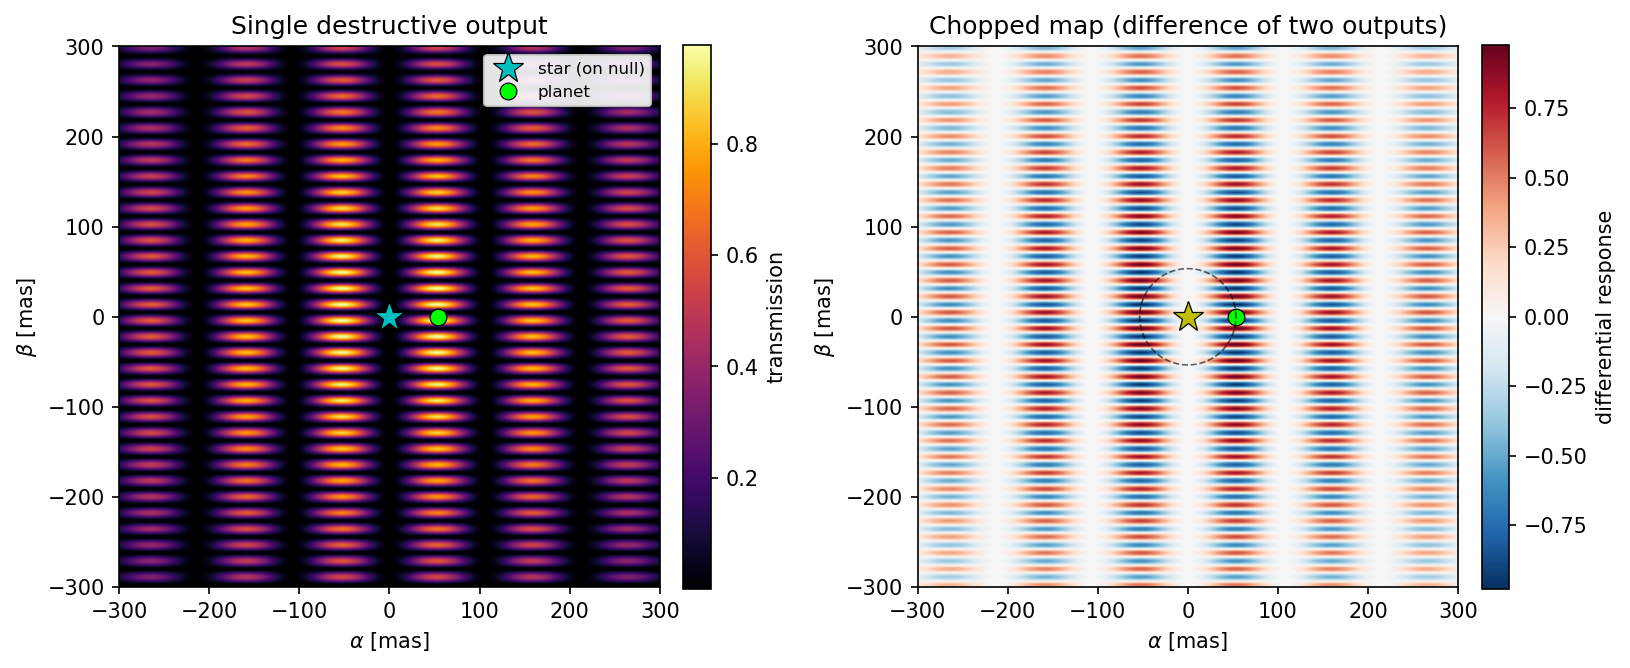
\includegraphics[width=\linewidth]{images/intro/transmission_maps.png}
        \caption{Transmission maps of the double Bracewell array.}
        \label{fig: transmission maps a}
    \end{subfigure}

    \vspace{2mm}

    \begin{subfigure}{.72\textwidth}
        \centering
        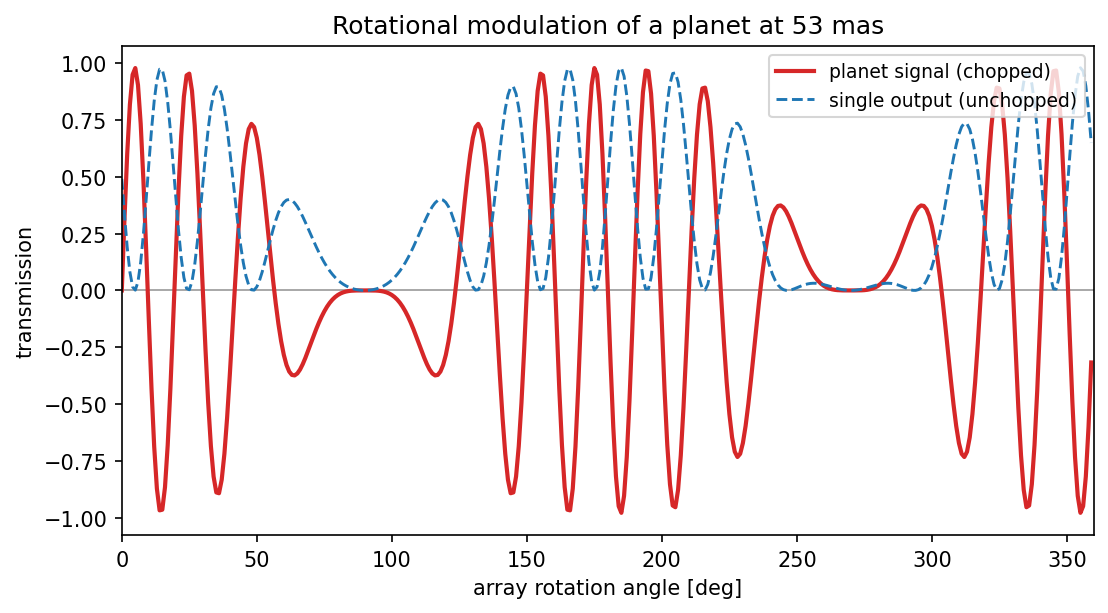
\includegraphics[width=\linewidth]{images/intro/transmission_modulation.png}
        \caption{Rotational modulation of the marked planet.}
        \label{fig: transmission maps b}
    \end{subfigure}
    \caption{Signal collection \DIFdelbeginFL \DIFdelFL{of }\DIFdelendFL \DIFaddbeginFL \DIFaddFL{in }\DIFaddendFL the \DIFdelbeginFL \DIFdelFL{LIFE double Bracewell array, computed directly with the LIFEsim transmission module }\DIFdelendFL \DIFaddbeginFL \DIFaddFL{double-Bracewell reference geometry }\DIFaddendFL at \DIFdelbeginFL \DIFdelFL{a wavelength of }\DIFdelendFL $10.4\,\upmu$m\DIFaddbeginFL \DIFaddFL{, $b=20\,$m }\DIFaddendFL and \DIFdelbeginFL \DIFdelFL{a nulling }\DIFdelendFL \DIFaddbeginFL \DIFaddFL{nominal }\DIFaddendFL baseline \DIFdelbeginFL \DIFdelFL{of $20\,$m}\DIFdelendFL \DIFaddbeginFL \DIFaddFL{ratio $r=6$}\DIFaddendFL , zoomed to the central \DIFdelbeginFL \DIFdelFL{$\pm 300\,$}\DIFdelendFL \DIFaddbeginFL \DIFaddFL{$\pm300\,$}\DIFaddendFL mas\DIFdelbeginFL \DIFdelFL{of the field of view}\DIFdelendFL . (a) \DIFdelbeginFL \DIFdelFL{Left: the transmission map of a }\DIFdelendFL \DIFaddbeginFL \DIFaddFL{A }\DIFaddendFL single \DIFdelbeginFL \DIFdelFL{destructive output. The star (cyan) sits on the deep on-axis null, while a planet (green) at an angular separation of $53\,$mas falls onto a bright fringe }\DIFdelendFL \DIFaddbeginFL \DIFaddFL{destructive-output map }\DIFaddendFL and \DIFdelbeginFL \DIFdelFL{is transmitted. Right: the }\DIFdelendFL \DIFaddbeginFL \DIFaddFL{its }\DIFaddendFL chopped \DIFdelbeginFL \DIFdelFL{map, formed as the }\DIFdelendFL difference\DIFdelbeginFL \DIFdelFL{of the two destructive outputs}\DIFdelendFL . \DIFdelbeginFL \DIFdelFL{It is antisymmetric, with positive (red) and negative (blue) lobes; any source symmetric about the line of sight cancels }\DIFdelendFL \DIFaddbeginFL \DIFaddFL{Symmetric mean contributions cancel }\DIFaddendFL in \DIFdelbeginFL \DIFdelFL{this }\DIFdelendFL \DIFaddbeginFL \DIFaddFL{the }\DIFaddendFL difference, whereas \DIFdelbeginFL \DIFdelFL{the }\DIFdelendFL \DIFaddbeginFL \DIFaddFL{an }\DIFaddendFL off-axis planet \DIFdelbeginFL \DIFdelFL{does not. The dashed circle traces }\DIFdelendFL \DIFaddbeginFL \DIFaddFL{generally has unequal transmission in }\DIFaddendFL the \DIFdelbeginFL \DIFdelFL{path the planet follows as the array rotates}\DIFdelendFL \DIFaddbeginFL \DIFaddFL{two outputs}\DIFaddendFL . (b) \DIFdelbeginFL \DIFdelFL{As }\DIFdelendFL \DIFaddbeginFL \DIFaddFL{Rotation modulates }\DIFaddendFL the \DIFdelbeginFL \DIFdelFL{array rotates, the planet is swept along that circle through the alternating lobes of the }\DIFdelendFL chopped \DIFdelbeginFL \DIFdelFL{map, so its collected }\DIFdelendFL \DIFaddbeginFL \DIFaddFL{planet }\DIFaddendFL signal\DIFdelbeginFL \DIFdelFL{(red) is modulated in time, while }\DIFdelendFL \DIFaddbeginFL \DIFaddFL{; }\DIFaddendFL the unchopped single-output response \DIFdelbeginFL \DIFdelFL{(blue dashed), through which the planetary photon noise is collected, carries }\DIFdelendFL \DIFaddbeginFL \DIFaddFL{used for its photon-noise term has }\DIFaddendFL a different weighting.\DIFdelbeginFL \DIFdelFL{The rich multi-lobe structure reflects the planet crossing the many fine fringes set by the imaging baseline; the essential point is that the planetary signal varies periodically in time while the symmetric backgrounds do not, which is what makes it separable.}\DIFdelendFL }
    \label{fig: transmission maps}
\end{figure}

Two consequences of this scheme carry directly into the SNR. First, the planetary \textit{signal} is collected through the chopped map, whereas the planetary \textit{photon noise}, which is insensitive to the sign of the modulation, is collected through a single, unchopped output; the two therefore enter with different transmission weights. Second, because the map is integrated over a full rotation, the effective response becomes radially symmetric and depends only on the angular separation of the planet and on the nulling baseline. This rotation-averaged response, further attenuated by a field-of-view taper that models the loss of off-axis coupling into the instrument's optical fibers, is the \textit{transmission efficiency} introduced in Section \ref{sec: intro: params}. \DIFdelbegin \DIFdel{With the collection mechanism established }\DIFdelend \DIFaddbegin \DIFadd{Having established what reaches the detector and how it is weighted}\DIFaddend , we can now \DIFdelbegin \DIFdel{make the notion of signal and noisequantitative}\DIFdelend \DIFaddbegin \DIFadd{quantify whether the planet can be distinguished from noise}\DIFaddend .

\subsection{The Signal-To-Noise Ratio (SNR)}
\DIFdelbegin \DIFdel{In data analysis, the }\textit{\DIFdel{signal-to-noise ratio}} %DIFAUXCMD
\DIFdel{(SNR ) is a simple measure of how noise-contaminated a signal is. Derived from the assumption of Gaussian signals, it is generally defined as
}\begin{align*}
    \DIFdel{\text{SNR} = \frac{\text{Usable Signal}}{\text{Total Noise}}.
}\end{align*}%DIFAUXCMD
\DIFdel{The astrophysical photon sources we are concerned with are generally non-monochromatic since we assume them to be dominated by black body physics. The SNR must hence be computed for each observed wavelength and then combined over the full spectrum. The final product is known as the }\textit{\DIFdel{bulk SNR}}%DIFAUXCMD
\DIFdel{. We only outline here the derivation of the LIFE mission bulk SNR by Dannert et al.
(2022).
}\DIFdelend \DIFaddbegin \DIFadd{The SNR is the expected modulated count signal divided by the standard deviation of the associated random count fluctuation. The implementation evaluates finite wavelength bins. Its reference planes are easy to confuse because planet flux is naturally specified at the observer, whereas extended backgrounds have already been integrated over collecting area. Table \ref{tab: snr symbols} makes the convention explicit.
}\DIFaddend 

\DIFdelbegin \DIFdel{In the context of the LIFE space mission, the signal is the pure photon flux from the target planet at the point of emission, filtered through the chopped transmission map. We denote any undesired photon fluxas noise, regardless of origin. The background noise contributions detailed in Section \ref{sec: intro: noise sources} are additive. Consider the background noise fluxes $N_1, N_2, ..., N_n$, then
the total background noise is given by
}\DIFdelend \DIFaddbegin \begin{table}[htbp]
\centering
\begin{tabular}{@{}lll@{}}
\toprule
\DIFaddFL{Symbol }& \DIFaddFL{Meaning at the SNR interface }& \DIFaddFL{Units }\\
\midrule
\DIFaddFL{$F_{p,i}$ }& \DIFaddFL{Planet photon flux at the collectors, integrated over bin $i$ }& \DIFaddFL{ph\,s$^{-1}$\,m$^{-2}$ }\\
\DIFaddFL{$A$ }& \DIFaddFL{Total effective collecting area in the source convention }& \DIFaddFL{m$^2$ }\\
\DIFaddFL{$\eta$ }& \DIFaddFL{Optical throughput times quantum efficiency }& \DIFaddFL{1 }\\
\DIFaddFL{$s_i$ }& \DIFaddFL{RMS chopped planet-response coefficient }& \DIFaddFL{1 }\\
\DIFaddFL{$n_i$ }& \DIFaddFL{RMS single-output planet-noise coefficient }& \DIFaddFL{1 }\\
\DIFaddFL{$B_i$ }& \DIFaddFL{Single-output astrophysical rate after area, before $\eta$ }& \DIFaddFL{ph\,s$^{-1}$ }\\
\DIFaddFL{$N_{I,i}$ }& \DIFaddFL{Added single-output rate after area, before $\eta$ }& \DIFaddFL{ph\,s$^{-1}$ }\\
\DIFaddFL{$t$ }& \DIFaddFL{On-source integration time }& \DIFaddFL{s }\\
\bottomrule
\end{tabular}
\caption{\DIFaddFL{SNR symbols and reference-plane convention. The reported spectral budget $N_I(\lambda)$ is converted to a bin rate by $N_{I,i}=N_I(\lambda_i)\Delta\lambda_i$.}}
\label{tab: snr symbols}
\end{table}

\DIFadd{For bin $i$, the expected chopped planet counts follow from its incident flux, collecting area, efficiency, time, and RMS modulation response. Each destructive output is a Poisson stream. If the two output counts have means $\mu_3$ and $\mu_4$, then
}\DIFaddend \begin{align}
\DIFdelbegin %DIFDELCMD < \label{eq: additive noise}
%DIFDELCMD <     %%%
\DIFdel{N_B}\DIFdelend \DIFaddbegin \DIFadd{\mathrm{Var}}\DIFaddend (\DIFdelbegin \DIFdel{\lambda}\DIFdelend \DIFaddbegin \DIFadd{C_3-C_4}\DIFaddend )=\DIFdelbegin \DIFdel{\sum_{i=1}^{n}N_i}\DIFdelend \DIFaddbegin \DIFadd{\mathrm{Var}}\DIFaddend (\DIFdelbegin \DIFdel{\lambda}\DIFdelend \DIFaddbegin \DIFadd{C_3}\DIFaddend )\DIFdelbegin \DIFdel{.
}\DIFdelend \DIFaddbegin \DIFadd{+\mathrm{Var}(C_4)=\mu_3+\mu_4
}\DIFaddend \end{align}
\DIFdelbegin \DIFdel{The mission has a finite spectral resolution, which means that the entire observed spectrum is separated into wavelength bins. All retrieved data are one-dimensional, only depending on the wavelength. Hence, we must compute an SNR for each bin with central wavelength $\lambda_i$. To average the signal and noise contributions per bin, we use the continuous root-mean-square (RMS). For the signal $S$ we have
}\DIFdelend \DIFaddbegin \DIFadd{when the streams are independent. Symmetric backgrounds have equal rotation-averaged rates in both outputs, so subtracting their means removes the DC signal but doubles their single-output variance. With $s_i=\sqrt{\langle(T_3-T_4)^2\rangle}$ and $n_i=\sqrt{\langle T_4^2\rangle}$, the implemented expected signal counts and variance are
}\DIFaddend \begin{align}
\DIFdelbegin \DIFdel{\text{RMS}_{\lambda_i, S} }\DIFdelend \DIFaddbegin \DIFadd{C_{S,i}}&\DIFaddend =\DIFdelbegin \DIFdel{\int}\DIFdelend \DIFaddbegin \DIFadd{F_{p,i}A\eta t s}\DIFaddend _i\DIFdelbegin \DIFdel{d \lambda \sqrt{\langle S^2(\lambda)\rangle}}\DIFdelend ,\DIFaddbegin \\
\DIFadd{V_i}&\DIFadd{=2\eta t}\left[\DIFadd{B_i+N_{I,i}+AF_{p,i}n_i}\right]\DIFadd{.
}\DIFaddend \end{align}
\DIFdelbegin \DIFdel{where $\int_i$ runs over the respective wavelength binand $\langle\cdot\rangle$ denotes the temporal average over one full array rotation, so that $\sqrt{\langle S^2(\lambda)\rangle}$ is the root-mean-square of the time-modulated chopped signal at each wavelength. Regarding noise, we must respect the background noise $N_B$, as well as the planetary noise $N_P$. The planetary noise denotes the emitted planetary photon flux filtered through the unchopped transmission map. Using that the background noise is constant in time, and taking the discrete RMS to combine the RMS of $N_B$ and $N_P$, we arrive at the RMS expression for the total non-systematic astrophysical noise per bin,
}\begin{align*}
    \DIFdel{\text{RMS}_{\lambda_i, N} = \sqrt{2\int_i d\lambda(N_B(\lambda) + \sqrt{\langle N_P^2(\lambda)\rangle})}.
}\end{align*}%DIFAUXCMD
\DIFdelend \DIFaddbegin \DIFadd{Hence
}\begin{align} \DIFadd{\label{eq: bin snr}
\mathrm{SNR}_i=\frac{C_{S,i}}{\sqrt{V_i}}.
}\end{align}\DIFaddend 
\DIFdelbegin \DIFdel{We may now compute the bin SNR as
}\begin{align*} \DIFdel{%DIFDELCMD < \label{eq: bin snr}%%%
    \text{SNR}_{\lambda_i} = \frac{\text{RMS}_{\lambda_i,
    S}}{\text{RMS}_{\lambda_i, N}} = \frac{\int_i d\lambda \sqrt{\langle S^2(\lambda)\rangle}}{\sqrt{2\int_i d\lambda(N_B(\lambda) + \sqrt{\langle N_P^2(\lambda)\rangle})}}.
}\end{align*}%DIFAUXCMD
\DIFdel{Finally, assuming that the noise between individual binsis uncorrelated}\DIFdelend \DIFaddbegin \DIFadd{Rates have units ph\,s$^{-1}$ per bin}\DIFaddend , \DIFaddbegin \DIFadd{$C_{S,i}$ is a count, $V_i$ a count variance, and $\sqrt{V_i}$ a count standard deviation. Chopping cancels the symmetric mean but subtracts two destructive outputs, so their independent photon-counting variances add and give the factor two. Output-swap/rotation symmetry makes the rotation-averaged single-output planet photon-noise rates equal; the same two-output variance sum therefore gives the factor two for the planet term. Assuming independent bins, }\DIFaddend the bulk SNR is
\DIFdelbegin \DIFdel{given by
}\DIFdelend \begin{align} \label{eq: bulk snr}
    \text{SNR}_\text{tot} = \sqrt{\sum_{\lambda_i}\text{SNR}_{\lambda_i}^2}.
\end{align}
\DIFaddbegin \DIFadd{It scales as $\sqrt{t}$; $\mathrm{SNR}_{1\mathrm{h}}$ uses $t=3600$\,s. This source-model convention follows LIFE paper II \mbox{%DIFAUXCMD
\cite{dannert2022life2}}\hskip0pt%DIFAUXCMD
. Correlated fluctuations and systematic biases are outside this photon-statistical model \mbox{%DIFAUXCMD
\cite{lay2004systematic,dannert2025thesis}}\hskip0pt%DIFAUXCMD
. }\DIFaddend From this point onward, \DIFdelbegin \DIFdel{the term SNR will always refer }\DIFdelend \DIFaddbegin \DIFadd{SNR refers }\DIFaddend to bulk SNR unless otherwise stated.

\DIFaddbegin \DIFadd{The SNR expression identifies the quantities that limit a measurement, but the error budget can only be defined after those noise contributions have been separated by physical origin.
}

\DIFaddend \subsection{Non-Systematic Noise Sources} \label{sec: intro: noise sources}
\DIFdelbegin \DIFdel{To be able to quantify the goals of the mission, we must carefully define some requirements on the performance of the instrument.
In particular, the nature of the instrument incurs noise sources. Firstly, in many solar systems, including our own, there is a circumsolar dust cloud emitting in the same wavelength range as the planet because it is at a comparable temperature. This noise is referred to as }\textit{\DIFdel{local-zodiacal}} %DIFAUXCMD
\DIFdel{if it originates from our solar system and }\textit{\DIFdel{exo-zodiacal}} %DIFAUXCMD
\DIFdel{if it is produced by the target system. Secondly, even if }\DIFdelend \DIFaddbegin \DIFadd{The model distinguishes noise by both physical origin and statistical treatment. Stellar leakage arises because a real star has finite angular radius: only its centre lies exactly on the null, while light from the resolved disk is transmitted. Local-zodiacal emission is thermal radiation from dust in the Solar System; exozodiacal emission is }\DIFaddend the \DIFaddbegin \DIFadd{analogous dust contribution around the }\DIFaddend target star\DIFdelbegin \DIFdel{is very far away, it will still have a non-zero apparent angular diameter. As the interferometer is designed to perfectly cancel out the starlight directly on the line of sight, the emission from the limb of the stellar disk will not be completely nulled. The resulting photon contribution is known as }\textit{\DIFdel{stellar leakage}}%DIFAUXCMD
\DIFdel{. Lastly, due to engineering limitations, the instrument itself is also certain to produce a signal contamination known as }\textit{\DIFdel{instrumental noise}}%DIFAUXCMD
\DIFdel{, such as dark currents on the detector. A sample of how astrophysical noise could look is shown in Fig.
\ref{fig: astronoise}.
}\DIFdelend \DIFaddbegin \DIFadd{. The adopted exozodiacal surface-brightness model follows the smooth, face-on disk prescription used in LIFEsim and is tied to established exozodiacal modeling \mbox{%DIFAUXCMD
\cite{kennedy2015,dannert2022life2}}\hskip0pt%DIFAUXCMD
. All three contribute photon shot noise even where chopping cancels their symmetric mean.
}\DIFaddend 

\DIFdelbegin %DIFDELCMD < \begin{figure}[htbp]
%DIFDELCMD < %%%
\DIFdelendFL \DIFaddbeginFL \begin{table}[htbp]
\DIFaddendFL \centering
\DIFdelbeginFL %DIFDELCMD < \begin{subfigure}{.49\textwidth}
%DIFDELCMD <   \centering
%DIFDELCMD <   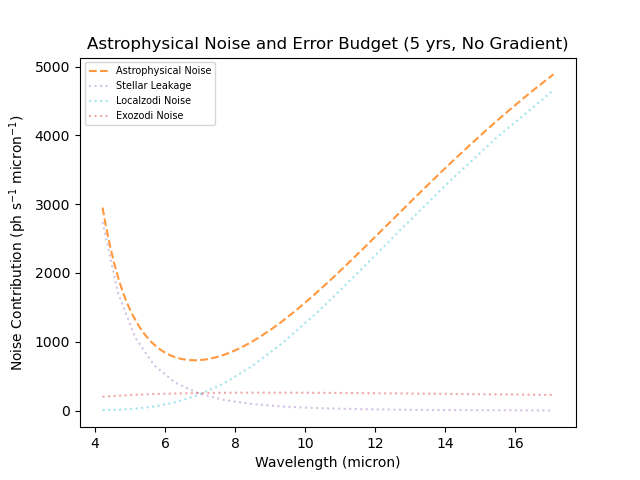
\includegraphics[width=\linewidth]{images/intro/constant_5yrs_noiseonly.png}
%DIFDELCMD <   %%%
%DIFDELCMD < \caption{%
{%DIFAUXCMD
\DIFdelFL{Stellar Leakage - Localzodi Dominated}}
%DIFAUXCMD
%DIFDELCMD < \end{subfigure}
%DIFDELCMD < \begin{subfigure}{.50\textwidth}
%DIFDELCMD <   \centering
%DIFDELCMD <   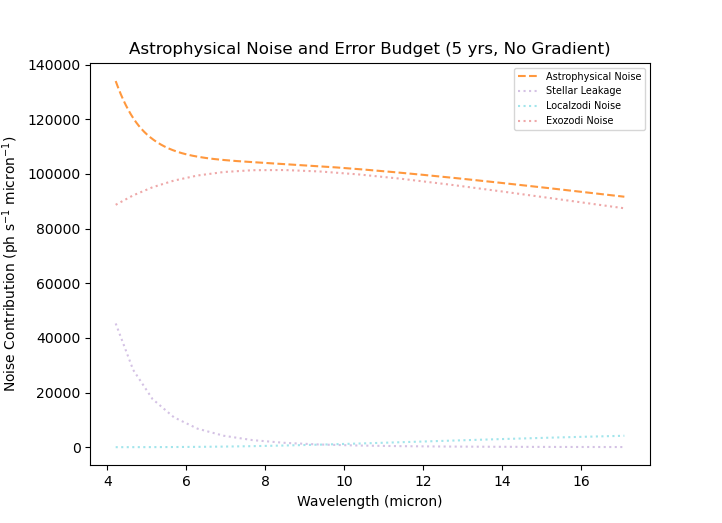
\includegraphics[width=\linewidth]{images/intro/constant_5yrs_noiseonly_exozodi.png}
%DIFDELCMD <   %%%
%DIFDELCMD < \caption{%
{%DIFAUXCMD
\DIFdelFL{Exozodi Dominated}}
%DIFAUXCMD
%DIFDELCMD < \end{subfigure}
%DIFDELCMD < %%%
%DIFDELCMD < \caption{%
{%DIFAUXCMD
\DIFdelFL{Demonstration of two typical astrophysical noise contributions over the LIFE mid-infrared spectrum. Stellar leakage dominates the shorter wavelengths, while the dust disks obscure the longer wavelengths. On the left hand side, we may see a typical low-exozodi case. In these cases a very typical minimum of astrophysical noise appears in the first third of the spectrum. A potential planetary signal would likely be clearly visible in the corresponding wavelength range. The right hand side displays a strongly exozodi-dominated system, which causes the noise to increase by roughly one order of magnitude everywhere in the spectrum. If a planet resides in this system, it will probably be very hard to characterize compared to the left case.}}
%DIFAUXCMD
%DIFDELCMD < \label{fig: astronoise}
%DIFDELCMD < \end{figure}
%DIFDELCMD < 

%DIFDELCMD < %%%
\DIFdel{The overall success of the mission depends on how well we can increase the SNR of the measurements. Although some noise may be mitigated by using photon statistics, we always strive to increase the SNR to be able to satisfactorily detect and characterize the maximum number of targets. In practice, if looking at a certain target yields data with a lot of noise , we cannot draw confident conclusions, which reduces the scientific benefit and might result }\DIFdelend \DIFaddbegin \begin{tabular}{@{}p{0.21\linewidth}p{0.24\linewidth}p{0.23\linewidth}p{0.23\linewidth}@{}}
\toprule
\DIFadd{Term }& \DIFadd{Physical origin }& \DIFadd{Modeled dependence }& \DIFadd{Treatment and boundary }\\
\midrule
\DIFadd{Stellar leakage }& \DIFadd{Finite stellar disk transmitted around the central null }& \DIFadd{$\lambda$, stellar radius and temperature, distance, $b$, null order }& \DIFadd{Uniform circular disk; photon noise only }\\
\DIFadd{Local zodiacal }& \DIFadd{Solar-System dust foreground }& \DIFadd{$\lambda$, target ecliptic latitude, field of view }& \DIFadd{Locally uniform circular foreground; photon noise only }\\
\DIFadd{Exozodiacal }& \DIFadd{Dust }\DIFaddend in the target \DIFdelbegin \DIFdel{being unsuitable. Subsequently, another target must be selected and its spectra retrieved, which takes more mission time. Due to this effect, we must aim to reduce all noise as much as possible. Now, the considered non-systematic astrophysical noise is governed by black-body physics and is created outside the instrument at its respective source, which gives us only limited optimization chances. Instrumental noise, however, is based on the construction and precision of the instrument itself, which we can directly influence. The question now arises of exactly }\DIFdelend \DIFaddbegin \DIFadd{system }& \DIFadd{$\lambda$, stellar luminosity and distance, disk radius }& \DIFadd{Smooth face-on axisymmetric disk; photon noise only }\\
\DIFadd{Planet }& \DIFadd{Desired thermal emission }& \DIFadd{$\lambda$, radius, temperature, separation and rotation }& \DIFadd{Chopped signal plus its own photon noise }\\
\DIFadd{Added budget $N_I$ }& \DIFadd{Equivalent aggregate instrument contribution }& \DIFadd{Imposed spectral family and amplitude }& \DIFadd{Independent Poisson-like variance at the pre-efficiency single-output plane }\\
\DIFadd{Excluded terms }& \DIFadd{Calibration bias, drift, correlated instability, confusion }& \DIFadd{Architecture and data-reduction dependent }& \DIFadd{Not represented by $N_I$ }\\
\bottomrule
\end{tabular}
\caption{\DIFadd{Noise taxonomy and model boundary \mbox{%DIFAUXCMD
\cite{dannert2022life2,kennedy2015}}\hskip0pt%DIFAUXCMD
. ``Photon noise only'' means that a source's mean chopped signal may cancel while the associated shot-noise variance remains. Excluded systematic and instability terms require a separate architecture-dependent treatment \mbox{%DIFAUXCMD
\cite{lay2004systematic,dannert2025thesis}}\hskip0pt%DIFAUXCMD
.}}
\label{tab: noise taxonomy}
\end{table}

\DIFadd{The question is }\DIFaddend how much instrumental \DIFdelbegin \DIFdel{noise we can allow }\DIFdelend \DIFaddbegin \DIFadd{random noise can be allowed }\DIFaddend in addition to the astrophysical \DIFdelbegin \DIFdel{noise for the mission goals to still be achievable in reasonable time. This total amount of noise allowed for a given mission time is known as the }\DIFdelend \DIFaddbegin \DIFadd{backgrounds while retaining the adopted mission target. Here the }\DIFaddend \textit{\DIFaddbegin \DIFadd{random-noise }\DIFaddend error budget} \DIFdelbegin \DIFdel{and plays a critical role in determining the engineering accuracy required for the instrument. It is essential to carefully assign this budget to ensure the success of the mission}\DIFdelend \DIFaddbegin \DIFadd{is operationally an equivalent added single-destructive-output photon-rate spectral density $N_I(\lambda)$, in ph\,s$^{-1}$\,$\upmu$m$^{-1}$, referred to the same pre-efficiency plane as the astrophysical background. It represents independent Poisson-like random terms that enter as additive variance after differencing. It neither represents correlated or systematic biases nor assigns the allowance to individual subsystems. To turn that budget into an engineering question, we next express the physical contributions as parameters that can be varied or held fixed}\DIFaddend .

\subsection{Parameters and Instrument Performance} \label{sec: intro: params}
\DIFdelbegin \DIFdel{In order to understand the methods we use, it is important to first define some terms. In the context of this work, we denote by a }\textit{\DIFdel{parameter}} %DIFAUXCMD
\DIFdelend \DIFaddbegin \DIFadd{A }\textit{\DIFadd{parameter}} \DIFadd{is }\DIFaddend a value or function \DIFdelbegin \DIFdel{that describes an aspect of the mission that we may or must vary and find constraints for . As an example , we should vary the limiting magnitudeand find a reasonable cutoff, hence it is a parameter. The wavelength binning of the instrument, on the other hand, is fixed in the mission itself and is hence not considered a parameter.
We must also distinguish between variable and agnostic parameters. The stellar leakage, for example, is variable because it depends on the distance and temperature of the star as well as the observed wavelength, since stars are much hotter than planets and hence emit more strongly in shorter wavelengths. Conversely, the limiting magnitude is agnostic, because it defines a cut-off above which we consider target stars invisible to any instrument we build. We must declare our approach based on whether a parameter is variable or agnostic.
}%DIFDELCMD < 

%DIFDELCMD < %%%
\DIFdel{Looking at the previously described astrophysical noise sources and assuming an ideal instrument without instrumental noise, we can compute the received photon counts for any instrument architecture, source and target. We can now return to the concept of an error budget: we distribute the budget by padding each parameter with a variable amount of margin. For our mission, we define the zero-noise-budget instrument as the absolute limit. Building a better instrument is impossible because it would require reducing the astrophysical photon flux. As the easiest instrument to build, it is therefore also our starting point. From there, we increase the permissible error budget by adding a margin to each parameter. }\DIFdelend \DIFaddbegin \DIFadd{used to describe a candidate mission calculation. A }\textit{\DIFadd{variable}} \DIFadd{parameter is a target-dependent physical signal or noise channel; changing it triggers SNR recomputation (for example stellar leakage or planetary transmission). An }\textit{\DIFadd{agnostic}} \DIFadd{parameter is a global visibility filter or overhead applied without recomputing source physics (for example limiting magnitude, field of regard, or slew time).
}

\DIFadd{The ideal $N_I=0$ case is the physical lower bound: it has maximum SNR and minimum mission time, but it is the }\textit{\DIFadd{hardest}} \DIFadd{engineering requirement because it demands a perfectly noiseless added contribution. It is a mathematical reference origin, not an easy design. Negative budgets are outside this model. Requirements are relaxed upward from this origin until the iso-mission-time boundary is reached. }\DIFaddend If, at some wavelength, the added budget is lower than the total astrophysical noise, \DIFdelbegin \DIFdel{we say that the instrument }\DIFdelend \DIFaddbegin \DIFadd{the calculation }\DIFaddend is \textit{astrophysical-noise-limited} \DIFdelbegin \DIFdel{at that wavelength. Conversely, should the budget exceed the total astrophysical noise, the instrument will be }\DIFdelend \DIFaddbegin \DIFadd{there; if it exceeds it, it is }\DIFaddend \textit{instrumental-noise-limited}\DIFdelbegin \DIFdel{there}\DIFdelend .

As an example, consider again the stellar leakage. Typically, a star emits more strongly in the shorter wavelengths, so we might add some margin to the shorter wavelengths and observe the impact on mission time. This \DIFdelbegin \DIFdel{example as well as the general budget distribution idea is illustrated in Fig. \ref{fig: leakage budget example}}\DIFdelend \DIFaddbegin \DIFadd{motivates the short-weighted ramp tested in Section \ref{sec: tse}; the opposite ramp tests the zodiacal-dominated long wavelengths. Neither shape redistributes or subtracts noise elsewhere}\DIFaddend .

\DIFdelbegin %DIFDELCMD < \begin{figure}[htbp]
%DIFDELCMD <     \centering
%DIFDELCMD <     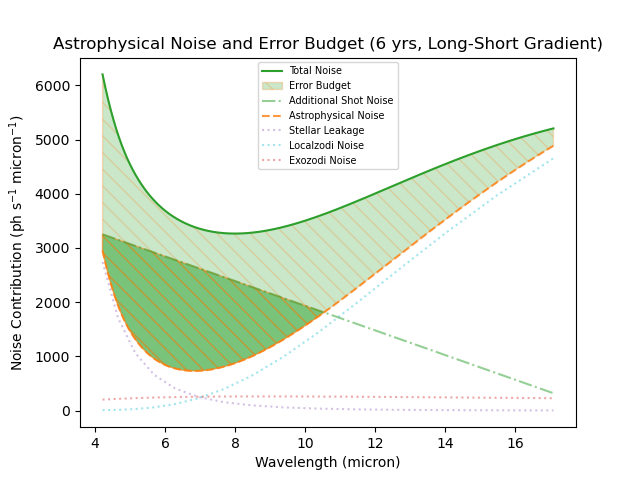
\includegraphics[width=0.8\linewidth]{images/intro/long_short_6yrs.png}
%DIFDELCMD <     %%%
%DIFDELCMD < \caption{%
{%DIFAUXCMD
\DIFdelFL{A simple budget distribution example. We pad the short wavelengths with budget to account for stellar leakage, proportionally subtracting it from the longer wavelengths in the process. The green-shaded area and dashed green line are the error budget we add on top, symbolizing instrumental noise. The shades of green denote whether the instrument is instrumental-noise- or astrophysical-noise-limited at any given wavelength. As an example, at 8 microns, the budget is higher than the astrophysical noise, so the instrument is instrumental-noise-limited. At 16 microns, the budget is lower than the astrophysical noise, so we say that the instrument is astrophysical-noise-limited there.}}
    %DIFAUXCMD
%DIFDELCMD < \label{fig: leakage budget example}
%DIFDELCMD < \end{figure}
%DIFDELCMD < 

%DIFDELCMD < %%%
\DIFdel{A special case is the planetary emission . It is related to the instrument through the transmission efficiency, which is a product of the fully rotated, hence radially symmetric, instrument transmission and the field of view taper. The former fundamentally depends on the nulling baseline, the physical distance between the interferometer apertures. The latter describes the signal loss as the photon incidence angle is shifted from the central axis as a result of optical fiber coupling. The emissions from the planet constitute our signal, which we desire to maximize}\DIFdelend \DIFaddbegin \DIFadd{Planetary emission enters through the rotation-averaged transmission efficiency and a common field-of-view taper. As defined in Section \ref{sec: intro: signal collection}, $b$ sets the null envelope and $rb$ the fine fringes in nominal settings; $b$ is selected per star from the habitable-zone centre and clipped to the allowed bounds. The field-of-view taper represents common off-axis coupling loss without assuming a particular taper formula}\DIFaddend .

We can now collect the complete set of variable parameters and the physical quantities each of them depends on. Every noise contribution reaches the instrument through the transmission map, which is why each additionally carries the wavelength dependence characteristic of its blackbody source. The variable parameters are as follows:
\begin{itemize}
    \item Stellar leakage. Depends on the wavelength, the stellar temperature, the stellar radius, and the distance to the star.
    \item Local-zodiacal noise. Depends on the wavelength and the ecliptic latitude of the target.
    \item Exo-zodiacal noise. Depends on the wavelength, the stellar luminosity, and the distance to the star.
    \item Planetary signal. Depends on the wavelength and, through the transmission efficiency, on the nulling baseline and the field of view taper.
\end{itemize}
This enumeration \DIFdelbegin \DIFdel{already indicates the size of the raw problem. Each variable parameter carries both }\DIFdelend \DIFaddbegin \DIFadd{specifies the raw dimension more precisely. Four physical channels each carry }\DIFaddend a multiplicative and an additive modifier\DIFdelbegin \DIFdel{(Section \ref{sec: intro: varparams descr}), and each modifier is in principle a free function of the two to four physical quantities listed above. Treated without simplification, the variable part of the trade space is therefore not merely high-dimensional but }\DIFdelend \DIFaddbegin \DIFadd{, giving up to eight free functions of their listed physical variables. Together with the three scalar agnostic parameters, the unrestricted problem is }\DIFaddend formally infinite-dimensional \DIFdelbegin \DIFdel{, since a }\DIFdelend \DIFaddbegin \DIFadd{because each }\DIFaddend free function has infinitely many degrees of freedom. \DIFdelbegin \DIFdel{This is precisely the observation that }\DIFdelend \DIFaddbegin \DIFadd{The reduced calculations reported here are much smaller: for fixed catalog, null order, operating point, and spectral family, the search is one-dimensional in amplitude $A$; including magnitude, field of regard, and slew time gives four scalar dimensions; allowing the two ramp endpoints to vary independently gives five. Catalog, null order, spectral family, and target mission time remain discrete scenario choices. This hierarchy }\DIFaddend motivates the reductions of Section \ref{sec: ts reduction: condensation}\DIFdelbegin \DIFdel{, which collapse these modifiers into a single, interpretable, one-dimensional noise function of wavelength}\DIFdelend .

In addition to the variable ones, there are \DIFdelbegin \DIFdel{also parameters that are inherently instrument-agnostic. They should also be varied and will impact the required mission time. Since they are agnostic and inherently one-dimensional, we will evaluate them }\DIFdelend \DIFaddbegin \DIFadd{parameters termed }\textit{\DIFadd{agnostic}}\DIFadd{: global filters or overheads scanned without recomputing source physics, not quantities literally independent of every architecture. They are evaluated }\DIFaddend on simple grids. The agnostic parameters are as follows:
\begin{itemize}
    \item Limiting magnitude. Describes the maximum K-band magnitude object that the instrument can detect.
    \item Field of regard. \DIFdelbegin \DIFdel{Describes a fundamental limit on the rotating instrument, excluding part of the celestial sphere. In practice, at any point in time, the instrument can only see part of the sky. We now observe which part of the sky is unobservable while the rotating instrument orbits the sun. We ultimately find that the celestial sphere beyond a certain ecliptic latitude is inaccessible to our observations. The field of regard symmetrically defines the allowed zone, with $\frac{\pi}{2}$ }\DIFdelend \DIFaddbegin \DIFadd{The implemented filter marks a target visible when its absolute ecliptic latitude is at most the FoR. Thus FoR $65^\circ$ retains the band from $-65^\circ$ to $+65^\circ$ and excludes the polar caps; FoR $\pi/2$ retains }\DIFaddend the full sky.
    \item Slew time. Defines the average time it takes for the instrument to center on a new target.
\end{itemize}
Knowing the starting points and limits, we can now go back to the performance of the instrument. We employ a practical science iso-performance approach. Specifically, we declare an instrument better-performing if it can complete the scientific goals of the mission in less time. The variable and agnostic parameters together span a large space of possible choices, which we call the \textit{trade space}. To \DIFdelbegin \DIFdel{be able to estimate the }\DIFdelend \DIFaddbegin \DIFadd{estimate an }\DIFaddend error budget, \DIFdelbegin \DIFdel{we must first create a tool that takes the parameters as input and gives the mission time as output. This tool is the }\DIFdelend \DIFaddbegin \DIFadd{the }\DIFaddend \textit{Agnostic Mission Simulator} (AMS), described in \DIFdelbegin \DIFdel{detail in }\DIFdelend Section \ref{sec: methods: AMS}\DIFdelbegin \DIFdel{. Hence, for this part, we invert the research question and strive to find the mission timefor a set error budget . The term "set" in this context also includes the distribution of the budget across all }\DIFdelend \DIFaddbegin \DIFadd{, maps inputs to mission time. Here a set budget means a specified wavelength-dependent additive shape together with selected agnostic operating }\DIFaddend parameters.

\subsection{The Trade Space} \label{sec: intro: trade space}
\DIFdelbegin \DIFdel{With the AMS in place, we can return to the fundamental question. How do we find the error budget for any set mission time? In theory, this would require inverting the AMS. In practice, it means scanning the trade space for the minimum mission time. Since we start the variable parameters from the astrophysical limits, we know that the mission time will increase monotonically by adding budget. Setting the error budget will hence be a question of just how much we can increase the budget before the mission simply takes too long. This sounds straightforward but undoubtedly requires a lot of creative thinking. Let us illustrate this with an example. We know that the trade space is very large - if we conservatively assume 10 degrees of freedom (variable parameter dimensions plus agnostic parameters), brute-force computing just 10 points for any degree of freedom, we end up with a grid of }\DIFdelend \DIFaddbegin \DIFadd{The parameters define a forward map from an instrument description to mission time, but the engineering question asks for its inverse: the largest added budget compatible with a chosen time. The raw space cannot be sampled directly because it contains free functions. Even a finite ten-dimensional surrogate, sampled at only ten values per dimension, would require }\DIFaddend $10^{10}$ \DIFdelbegin \DIFdel{points, on each of which the AMS must run once. Assuming a very optimistic parallelized AMS runtime of }\DIFdelend \DIFaddbegin \DIFadd{AMS evaluations. At an optimistic }\DIFaddend one second per \DIFdelbegin \DIFdel{data point, we are looking at a total runtime of }\DIFdelend \DIFaddbegin \DIFadd{evaluation, that coarse grid would take approximately }\DIFaddend 317 years\DIFdelbegin \DIFdel{(!), by which time we get an extremely coarse overview of the trade space . As this little example drastically shows , we require a more refined approach to trade space exploration (TSE).
A conceivable approach may be to combine variable parameters in order to reduce the trade space.
}\DIFdelend \DIFaddbegin \DIFadd{. This estimate is illustrative rather than a claim that the raw functional space has exactly ten dimensions. It shows why the workflow must first restrict the budget to interpretable spectral families, then exploit monotonic searches and reusable computations instead of applying a uniform grid.
}\DIFaddend 

\DIFdelbegin \DIFdel{Once the TSE tool is also sufficiently implemented, we can run it for each of the previously found instrument architectures and then compare the resulting error budgets. In addition to defining an error budget for the instrument, this would undoubtedly also give valuable insight into which architecture is more suitable for the mission}\DIFdelend \DIFaddbegin \DIFadd{The completed TSE runs invert this mapping for null orders two and four. They therefore show both how much aggregate random-noise amplitude is tolerated within each tested shape and how the modeled null order changes the spectral ordering of those allowances}\DIFaddend .

\DIFdelbegin %DIFDELCMD < \newpage
%DIFDELCMD < %%%
\section{\DIFdel{Methods}} %DIFAUXCMD
\addtocounter{section}{-1}%DIFAUXCMD
\DIFdelend \DIFaddbegin \chapteropening{Methods}{Building a fixed-reference simulator and a controlled null-order proxy} \DIFaddend \label{sec: methods}
\DIFdelbegin \DIFdel{With the groundwork covered, we can now actually talk about the aforementioned instrument-agnostic approach. What does it mean to construct such an approach? How do we simulate and set constraints on instrument physics without actually knowing the instrument?
}\DIFdelend \DIFaddbegin \DIFadd{The background has established the quantities mapped from a fixed double-Bracewell reference description to mission time. We now construct that mapping, with a mechanism-agnostic aggregate random-noise allowance and the stated null-order proxy.
}\DIFaddend 

\subsection{Variable Parameter Treatment} \label{sec: intro: varparams descr}
\DIFdelbegin \DIFdel{In order to describe our approach, we must first determine how to implement the variable parameters. A conceivable strategy could be an interpolation grid on which the parameters are evaluated. Each point in the grid could be modified, granting an enormous trade space. This benefit, however, also constitutes the biggest drawback of this approach because such a large trade space will be difficult to confine, making TSE even more challenging}\DIFdelend \DIFaddbegin \DIFadd{A free interpolation grid would preserve maximum flexibility but create a poorly constrained functional search}\DIFaddend . Instead, \DIFdelbegin \DIFdel{we propose a relatively simple functional approach. Denoting by F the output photon flux density of a regular astrophysical model (i. e., the zero-budget planetary signal or astrophysical noise), we express the }\textit{\DIFdel{variable parameter}} %DIFAUXCMD
\DIFdel{V as
}\DIFdelend \DIFaddbegin \DIFadd{the AMS modifies each modeled photon-flux density $F$ through a multiplicative function $M$ and an additive function $A$:
}\DIFaddend \begin{align} \label{eq: variable parameter}
    \text{V}(\alpha_1, \dots, \alpha_n) = \text{M}(\alpha_1, \dots, \alpha_n) \times \text{F} + \text{A}(\alpha_1, \dots, \alpha_n),
\end{align}
where \DIFdelbegin \DIFdel{we define M as the }\textit{\DIFdel{multiplicative modifier}} %DIFAUXCMD
\DIFdel{and A as the }\textit{\DIFdel{additive modifier}}%DIFAUXCMD
\DIFdel{. The dependencies $\alpha_i$ stand for arbitrary physical quantities like wavelength, stellar radius, etc. In this context, increasing either M or A would increase V, thus assigning some budget to V. Notice here that we must have $\text{M} \geq 1$ and $\text{A} \geq 0$, because otherwise we would reduce the pure astrophysical flux, which is impossible. Referring to Section \ref{sec: intro: params}, our }\DIFdelend \DIFaddbegin \DIFadd{M is a multiplicative modifier and A an additive modifier. For an }\textit{\DIFadd{extra-noise}} \DIFadd{channel, $M\geq1$ and $A\geq0$ preserve the astrophysical reference, with the }\DIFaddend zero-budget \DIFdelbegin \DIFdel{parameter is defined as $\text{M} = 1$ and $\text{A} = 0$. }\DIFdelend \DIFaddbegin \DIFadd{case $M=1$, $A=0$. These inequalities do not describe signal degradation: that requires a separate convention, such as $0\leq M\leq1$ or a negative additive term constrained to keep the signal non-negative. The condensed study reported here varies additive background noise only.
}\DIFaddend 

\subsection{Modified Double Bracewell Null Depth Approach} \label{sec: intro: null depth approach}
\DIFdelbegin \DIFdel{Computing the signal and contribution for any nulling architecture, and hence conducting a "true" agnostic approach, is neither reasonably feasible nor interesting. Since we know that we will build a rotating nulling interferometer, there is only a finite number of realizations. Implementing a choice of these realizations is also not helpful because we might put too much emphasis on certain architectures while omitting others. Also, parameters like the baseline may become multi-dimensional, asymmetrical, and hard to define. We therefore propose a different and simpler approach to architecture selection. We know the transmission map of the double Bracewell interferometer, whose dark outputs have the form
}\begin{align*}
    \DIFdel{T\ \propto\ \text{sin}^2(\phi)\times \text{cos}^2(\psi),
}\end{align*}%DIFAUXCMD
\DIFdel{where $\phi$ }\DIFdelend \DIFaddbegin \DIFadd{The transmission proxy is architecture-parameterized with respect to null order, while remaining mechanism-agnostic only for the aggregate random-noise allowance. For the reference double Bracewell, the first pairwise combinations produce a $\sin^2$ nulling envelope, while the second combination produces complementary imaging fringes. Let $\alpha$ }\DIFaddend and \DIFdelbegin \DIFdel{$\psi$ are functions depending on wavelength and baseline. To approximate a different order null, we now change the form to }\begin{align*}
    \DIFdel{T_n\ \propto \text{sin}^n(\phi)\times \text{cos}^2(\psi),
}\end{align*}%DIFAUXCMD
\DIFdelend \DIFaddbegin \DIFadd{$\beta$ be angular sky offsets along the nulling and imaging-baseline directions. With the LIFE notation $b$ for nulling baseline and $r$ for the imaging-to-nulling baseline ratio \mbox{%DIFAUXCMD
\cite{dannert2022life2}}\hskip0pt%DIFAUXCMD
, the phases are $\phi=\pi b\alpha/\lambda$ and $\psi=\pi rb\beta/\lambda$. The two reference destructive outputs are
}\begin{align}
\DIFadd{T_{3,2}}&\DIFadd{=\sin^2(\phi)\cos^2(\psi-\pi/4),}\\
\DIFadd{T_{4,2}}&\DIFadd{=\sin^2(\phi)\cos^2(\psi+\pi/4).
}\end{align}\DIFaddend 
\DIFdelbegin \DIFdel{where $n$ denotes the null order. The functions $\phi$ and $\psi$ depend linearly on the angular offset from the line of sight.
Hence, on the line of sight, it holds that
}\begin{align*}
    \DIFdel{\phi = \psi = 0 \implies T_n = 0.
}\end{align*}%DIFAUXCMD
\DIFdelend \DIFaddbegin \DIFadd{Their difference is $T_{3,2}-T_{4,2}=\sin^2(\phi)\sin(2\psi)$, up to the chosen output-sign convention. Close to the optical axis, $\sin\phi\simeq\phi$, so the nulling envelope grows as $\phi^2$ and has intensity null order two.
}

\DIFadd{The proxy replaces only this envelope by $\sin^n\phi$:
}\begin{align}
\DIFadd{T_{3,n}}&\DIFadd{=\sin^n(\phi)\cos^2(\psi-\pi/4),}&
\DIFadd{T_{4,n}}&\DIFadd{=\sin^n(\phi)\cos^2(\psi+\pi/4).
\label{eq: null proxy outputs}
}\end{align}\DIFaddend 
\DIFdelbegin \DIFdel{As desired, the transmission vanishes on the line of sight and increases radially in }\DIFdelend \DIFaddbegin \DIFadd{It accepts positive even }\DIFaddend $n$\DIFdelbegin \DIFdel{th order, simulating $n$th order nulling. With this ansatz, we may continue to use the double Bracewell baseline formalism and physics, but we get a null form and depth near the line of sight akin to different architectures with different null order. This approach, while very crude, allows us to study the impact of changing null order on the total mission time, which is especially relevant for on-axis noise sources like stellar leakage}\DIFdelend \DIFaddbegin \DIFadd{. Table \ref{tab: proxy boundary} separates the controlled change from the quantities deliberately held fixed.
}

\begin{table}[htbp]
\centering
\begin{tabular}{@{}p{0.44\linewidth}p{0.44\linewidth}@{}}
\toprule
\DIFaddFL{Changed by the proxy }& \DIFaddFL{Preserved between orders }\\
\midrule
\DIFaddFL{Near-axis intensity power $\sin^2\phi\rightarrow\sin^4\phi$ }& \DIFaddFL{Four collectors and collecting area }\\
\DIFaddFL{Stellar and extended-background transmission }& \DIFaddFL{Optical throughput and detector efficiency }\\
\DIFaddFL{Planet signal and photon-noise transmission }& \DIFaddFL{Imaging phase, baseline ratio $r=6$, and rotation rule }\\
\DIFaddFL{Far-field average of the nulling envelope }& \DIFaddFL{Per-star baseline prescription and 10--100\,m bounds }\\
\bottomrule
\end{tabular}
\caption{\DIFaddFL{Interpretation boundary of the null-order proxy. No realizable beam-combination matrix, aperture rearrangement, or throughput renormalization is introduced for order four.}}
\label{tab: proxy boundary}
\end{table}

\DIFadd{This distinction is central. The proxy keeps four apertures, collecting area, efficiency, and baseline prescription fixed, but does not normalize throughput between orders. Thus $n=4$ has a lower asymptotic average transmission. The comparison intentionally combines stronger central suppression with the transmission change implied by Eq. \ref{eq: null proxy outputs}. It measures the consequence of that mathematical response, not the performance or feasibility of a specified fourth-order beam combiner}\DIFaddend .

\subsection{The Agnostic Mission Simulator (AMS)} \label{sec: methods: AMS}
\DIFdelbegin \DIFdel{As described in Section \ref{sec: intro: params}, the AMS serves to compute the mission time for any input of parameters. The simulator proceeds }\DIFdelend \DIFaddbegin \DIFadd{The AMS maps one parameter set to mission time }\DIFaddend in two phases. The \textit{simulation phase} \DIFdelbegin \DIFdel{combines an SNR flow, which computes each signal and noise source using regular models and the variable parameter approach described in Section \ref{sec: intro: varparams descr}, with a filter flow, which selects the results on the basis of the agnostic parameters. The subsequent }\DIFdelend \DIFaddbegin \DIFadd{computes or reuses an unfiltered one-hour SNR for every catalog planet, then applies the global visibility filters. The }\DIFaddend \textit{distribution phase} \DIFdelbegin \DIFdel{then uses these SNRs to distribute the observation time across the targets and return }\DIFdelend \DIFaddbegin \DIFadd{schedules the filtered targets and returns }\DIFaddend the required percentile mission time.
\DIFdelbegin \DIFdel{We now explain each phase in detail.
}\DIFdelend 

\subsubsection{The Simulation Phase}
\DIFdelbegin \DIFdel{This is the core of the AMS: the rapid evaluation of the SNR for the entire input planet catalog. The processing flow, illustrated in Fig. }\DIFdelend \DIFaddbegin \DIFadd{Figure }\DIFaddend \ref{fig: simphase flowchart} \DIFdelbegin \DIFdel{, is divided into two distinct components: the }\DIFdelend \DIFaddbegin \DIFadd{separates the expensive }\DIFaddend \textit{SNR flow} \DIFdelbegin \DIFdel{and the }\DIFdelend \DIFaddbegin \DIFadd{from the inexpensive }\DIFaddend \textit{filter flow}. The \DIFdelbegin \DIFdel{AMS uses an array, the AMS SNR array, to constantly store an SNR for each target in the catalog. The SNR flow now serves to compute this array based on the currently set variable parameters. Afterwards, the filter flow is run, during which the agnostic parameters are employed to return a filtered copy of the up-to-date AMS SNR array. The AMS continuously and automatically tracks whether any variable parameters have changed compared to the previous SNR flow. If they have, another SNR flow is triggered. If they have not been varied, however, only the filtering is performed}\DIFdelend \DIFaddbegin \DIFadd{SNR flow fills a persistent array with one-hour SNRs for every target and reruns only when a physics-governing quantity changes. The filter flow always returns a copy in which targets failing the magnitude or field-of-regard cut have SNR zero; it never overwrites the unfiltered cache}\DIFaddend .

\DIFdelbegin \DIFdel{In case }\DIFdelend \DIFaddbegin \DIFadd{When }\DIFaddend the SNR flow \DIFdelbegin \DIFdel{needs to be run, we perform a full unfiltered iteration over the entire target catalog. For each target, we compute the astrophysical noise contributions and the planetary signal through the variable parameters, finally combining all the values to get the target SNR. This value is then saved in an array. In this step, a key optimization is introduced by exploiting the structure of the underlying physics. Importantly, the noise contributions computed during the interpolation phase may be distinguished by their origin. The stellar leakageand }\DIFdelend \DIFaddbegin \DIFadd{runs, it iterates over the complete catalog. Within that recomputation, stellar leakage, }\DIFaddend local-zodiacal noise\DIFdelbegin \DIFdel{are fundamentally connected to the entire target system, while the planetary signal and noise (transmission efficiency) must be re-evaluated for every single target. We now compute the stellar physics only once for each distinct star and store the result in a memoization dictionary. This way, whenever we encounter another target around the same star, we may re-use the stellar physics and save time on the interpolator. As the loop progresses, the }\DIFdelend \DIFaddbegin \DIFadd{, and the unit-exozodi response are reused among planets sharing one host; planet transmission remains target-specific. Magnitude, field of regard, and slew-time changes reuse the unfiltered }\DIFaddend SNR array and \DIFdelbegin \DIFdel{the stellar memo dictionary will progressively complete. Once the loop terminates, we define the now complete array as our current AMS SNR array and conclude the SNR flow. }\DIFdelend \DIFaddbegin \DIFadd{rerun only filtering and time distribution. By contrast, any change to budget amplitude or spectral shape changes the bin variance, invalidates the SNR array, and requires catalog-wide SNR recomputation.
}\DIFaddend 

\DIFdelbegin \DIFdel{With an up-to-date AMS SNR array, we may proceed with the filter flow. The flow starts by creating an empty result array with an entry for each target planet, much like the SNR flow. We then iterate over the whole catalog again. If a target fulfills the agnostic filter requirements given by limiting magnitude and field of regard, its spot in the result array is set to the SNR from the AMS SNR array. In this case, we consider the target visible. If the target, however, does not meet both cutoff criteria, we set its SNR result to zero, considering the target invisible. The benefit of using a different arrayin this way is that we preserve the original AMS SNR array, much like a database. To illustrate the usefulness of this extra memory usage, assume that we first test a highly restrictive filter and then follow with an unfiltered run. If we overwrote the AMS SNR array, the unfiltered run would still have the values from the first run "deleted", thereby falsifying the result.
It is hence wise to only modify the AMS SNR array when completely re-computing it and leaving it constant otherwise. Once the filter flow terminates, we ultimately return the filtered result array, which concludes this phase.
}%DIFDELCMD < 

%DIFDELCMD < \begin{sidewaysfigure}
%DIFDELCMD <     %%%
\DIFdelend \DIFaddbegin \begin{landscape}
\begin{figure}[p]
    \DIFaddendFL \centering
    \DIFdelbeginFL %DIFDELCMD < 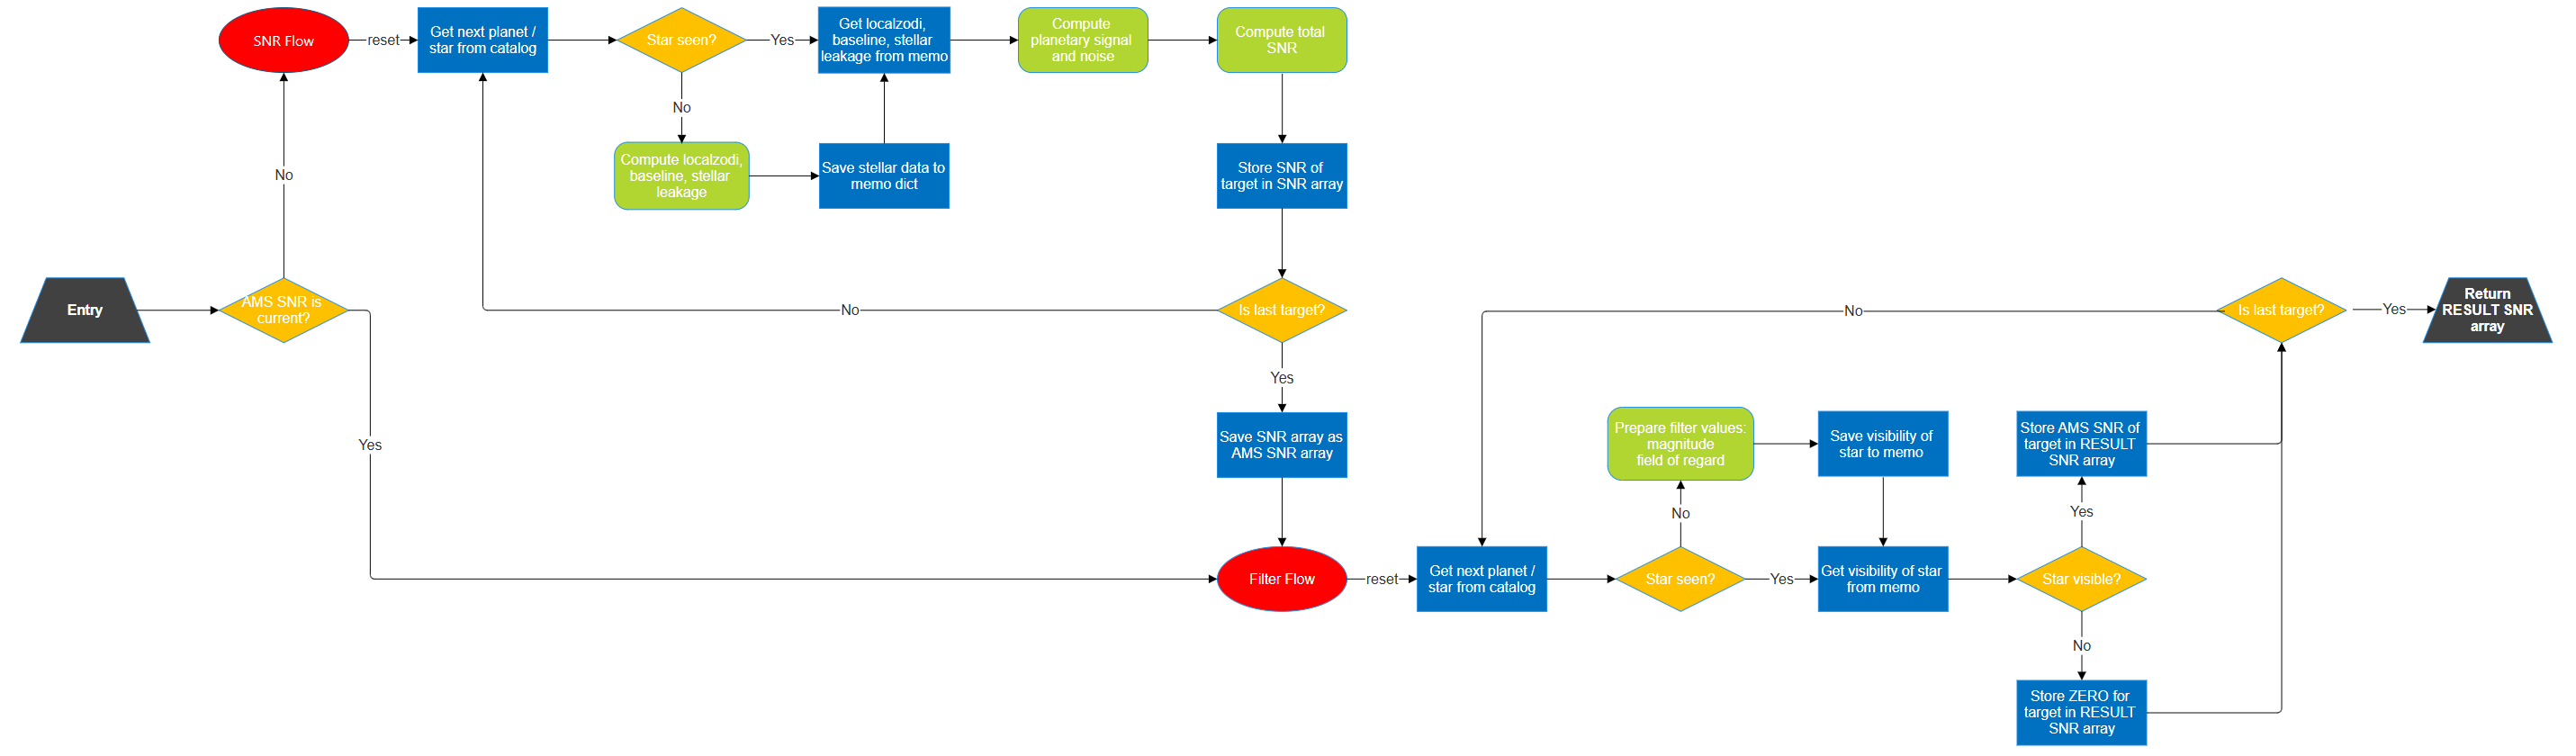
\includegraphics[width=0.95\textheight]{images/ams_flowchart_simphase.png}
%DIFDELCMD <     %%%
\DIFdelendFL \DIFaddbeginFL 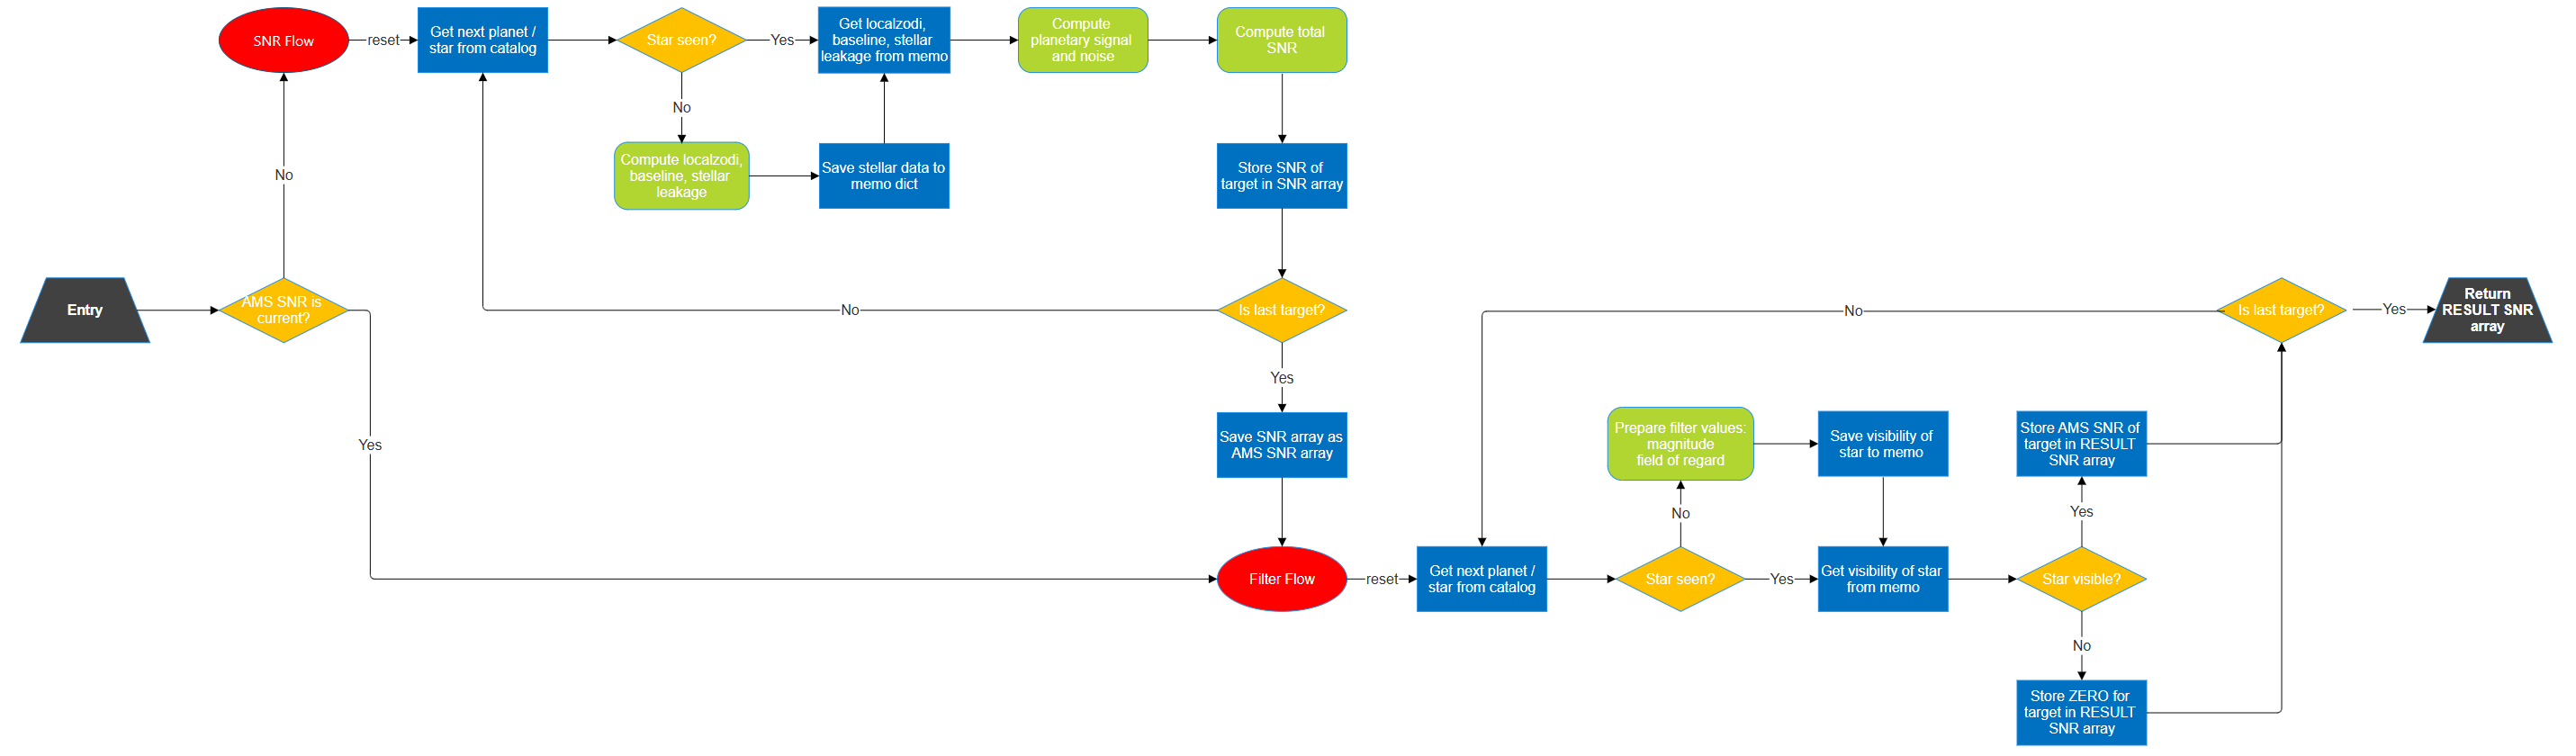
\includegraphics[width=0.95\linewidth]{images/ams_flowchart_simphase.png}
    \DIFaddendFL \caption{\DIFdelbeginFL \DIFdelFL{Flowchart of the }\DIFdelendFL AMS simulation phase. Gray \DIFdelbeginFL \DIFdelFL{trapezes refer to }\DIFdelendFL \DIFaddbeginFL \DIFaddFL{trapezoids mark }\DIFaddendFL entry or exit\DIFdelbeginFL \DIFdelFL{points}\DIFdelendFL , red tiles denote flows, yellow diamonds \DIFdelbeginFL \DIFdelFL{mark decision points}\DIFdelendFL \DIFaddbeginFL \DIFaddFL{decisions}\DIFaddendFL , green boxes \DIFdelbeginFL \DIFdelFL{define calculation steps}\DIFdelendFL \DIFaddbeginFL \DIFaddFL{calculations}\DIFaddendFL , \DIFaddbeginFL \DIFaddFL{and }\DIFaddendFL blue rectangles \DIFdelbeginFL \DIFdelFL{stand for }\DIFdelendFL memory \DIFdelbeginFL \DIFdelFL{manipulation}\DIFdelendFL \DIFaddbeginFL \DIFaddFL{operations}\DIFaddendFL . \DIFdelbeginFL \DIFdelFL{The }\textit{\DIFdelFL{SNR flow}} %DIFAUXCMD
\DIFdelFL{is run whenever the SNRs need to be re-computed, meaning after each physics-governing parameter change }\DIFdelendFL \DIFaddbeginFL \DIFaddFL{Physics }\DIFaddendFL or \DIFaddbeginFL \DIFaddFL{budget changes trigger }\DIFaddendFL the \DIFdelbeginFL \DIFdelFL{first time the AMS is run. At the end of the }\DIFdelendFL \DIFaddbeginFL \DIFaddFL{SNR }\DIFaddendFL flow \DIFdelbeginFL \DIFdelFL{, }\DIFdelendFL \DIFaddbeginFL \DIFaddFL{and replace }\DIFaddendFL the unfiltered \DIFdelbeginFL \DIFdelFL{SNRs are saved in the AMS for later use}\DIFdelendFL \DIFaddbeginFL \DIFaddFL{cache}\DIFaddendFL . The \DIFdelbeginFL \textit{\DIFdelFL{filter flow}} %DIFAUXCMD
\DIFdelFL{is }\DIFdelendFL \DIFaddbeginFL \DIFaddFL{filter flow }\DIFaddendFL always \DIFdelbeginFL \DIFdelFL{run }\DIFdelendFL \DIFaddbeginFL \DIFaddFL{copies that cache }\DIFaddendFL and \DIFdelbeginFL \DIFdelFL{uses }\DIFdelendFL \DIFaddbeginFL \DIFaddFL{sets targets outside }\DIFaddendFL the \DIFdelbeginFL \DIFdelFL{agnostic cutoff parameters, specifically }\DIFdelendFL magnitude \DIFdelbeginFL \DIFdelFL{and field of regard, }\DIFdelendFL \DIFaddbeginFL \DIFaddFL{or field-of-regard limits }\DIFaddendFL to \DIFdelbeginFL \DIFdelFL{set the SNR of unobservable targets to }\DIFdelendFL zero\DIFaddbeginFL \DIFaddFL{; it never destroys unfiltered values}\DIFaddendFL .\DIFdelbeginFL \DIFdelFL{The final output is the full set of filtered SNRs. Important: The filter flow does not change the SNRs from the SNR flow, but always makes a full copy in order not to lose any data through filtering.}\DIFdelendFL }
    \label{fig: simphase flowchart}
\DIFdelbeginFL %DIFDELCMD < \end{sidewaysfigure}
%DIFDELCMD < %%%
\DIFdelendFL \DIFaddbeginFL \end{figure}
\end{landscape}
\clearpage
\DIFaddend 

\subsubsection{The Distribution Phase}
We now have a full set of filtered SNRs for every target in the input planet catalog. The only remaining step is to use LIFEsim to distribute the available observation time across the targets and then find the required mission time.

The distribution rests on \DIFdelbegin \DIFdel{a single fact about }\DIFdelend photon-limited \DIFdelbegin \DIFdel{measurements: the SNR accumulates }\DIFdelend \DIFaddbegin \DIFadd{SNR accumulation }\DIFaddend as the square root of \DIFdelbegin \DIFdel{the }\DIFdelend integration time. The SNR flow yields \DIFdelbegin \DIFdel{, }\DIFdelend \DIFaddbegin \DIFadd{$\text{SNR}_{1\text{h}}$ }\DIFaddend for each target, \DIFdelbegin \DIFdel{the ratio $\text{SNR}_{1\text{h}}$ attainable in one hour of observation, so
after an integration time $t$ the accumulated ratio is $\text{SNR}(t) = \text{SNR}_{1\text{h}}\sqrt{t/1\,\text{h}}$, and separate visits to the same target add in quadrature. Reaching a required threshold $\text{SNR}_\text{req}$, the value of 44 assumed for a successful characterization in Experiment 1, from a current level $\text{SNR}_\text{cur}$ therefore costs an integration time of
}\begin{align*} \DIFdel{%DIFDELCMD < \label{eq: integration time}%%%
    t = \frac{\text{SNR}_\text{req}^2 - \text{SNR}_\text{cur}^2}{\text{SNR}_{1\text{h}}^2}\quad\text{[h]}.
}\end{align*}%DIFAUXCMD
\DIFdelend \DIFaddbegin \DIFadd{so
}\begin{align} \DIFadd{\label{eq: integration time}
    t_\mathrm{int}(q) = \left(\frac{q}{\text{SNR}_{1\text{h}}}\right)^2\quad\text{[h]}
}\end{align}\DIFaddend 
\DIFdelbegin \DIFdel{Each retargeting additionally incurs a fixed overhead, }\DIFdelend \DIFaddbegin \DIFadd{for a fresh integration to requested bulk SNR $q$. The implemented follow-up calculation does not subtract SNR already accumulated during detection. For a selected planet, with slew time $t_\mathrm{slew}$, it charges
}\begin{align}
\DIFadd{t_\mathrm{orbit}}&\DIFadd{=(n_\mathrm{orbits}-1)
\left[t_\mathrm{int}(7)+t_\mathrm{slew}\right],}\\
\DIFadd{t_\mathrm{char}}&\DIFadd{=t_\mathrm{int}(44.1)+t_\mathrm{slew}.
}\end{align}
\DIFadd{This convention treats the four follow-up orbit epochs and the characterization as separate observations. It is intentionally reported as implemented; alternative reuse of detection photons would reduce the follow-up cost.
}

\DIFadd{The complete scheduler is:
}\begin{enumerate}
    \item \DIFadd{Optimize one common detection sequence over all 100 synthetic universes.
    }\item \DIFadd{Stop when the inherited strict completion checks report more than 50 qualifying detections in more than 90\% of universes. With 100 universes, this means at least 51 planets in at least 91 universes.
    }\item \DIFadd{Assign the resulting shared detection-campaign time to every represented universe.
    }\item \DIFadd{In each universe, retain eligible planets that were detected, rank them by their one-hour SNR at maximum separation, and select the best 50.
    }\item \DIFadd{Add four orbit follow-ups and one characterization observation per selected planet using the equations above.
    }\item \DIFadd{Return the 90th percentile of the resulting per-universe total times.
}\end{enumerate}

\DIFadd{The AMS is consequently a perfect-information ensemble yield model, not an adaptive discovery scheduler. In experiment-limited mode, }\DIFaddend the \DIFdelbegin \DIFdel{slew time introduced as an agnostic parameter in Section \ref{sec: intro: params}, which is charged before any integration begins to count toward the SNR.
The targets are then scheduled greedily:
at each step the optimizer observes the star that yields the most new detections per unit of spent mission time }\DIFdelend \DIFaddbegin \DIFadd{configured 0.8 observing efficiency neither caps nor rescales the returned time. Here ``completion of Experiment~1'' always inherits the strict implementation above: at least 51 detections in at least 91 universes, with empty universes omitted from the time sheet. The strict inequalities tend to raise mission time}\DIFaddend , \DIFdelbegin \DIFdel{that is, the steepest gain in scientific return, and adds the corresponding integration and slew time to the running total.
    This continues until either the available observation budget, the product of the total search time and the observing efficiency, is exhausted, or the required number of targets has been characterized. We rely on the existing LIFEsim greedy optimizer for this step and do not reproduce its full internal logic here. }\DIFdelend \DIFaddbegin \DIFadd{whereas omission can bias the reported distribution low. Their net effect is not known from the retained outputs.
}\DIFaddend 

\DIFdelbegin \DIFdel{To define the mission time output, recall that the current input planet catalog simulates Kepler statistics to statistically assign hypothetical planets to known stars. Each assignment iteration constitutes one universe. Since the AMS computes the mission timeper universe, and the planets are different in each universe, the result must be a distribution of mission times across the universes. By the law of large numbers, the more universes there are in our catalog, the more closely we will approximate the true mission time distribution. We define our required mission timeresult, the final output of the AMS, by a certain percentile of completed missions. As an example, a }\DIFdelend \DIFaddbegin \DIFadd{The returned percentile is fixed at 90\%. If 100 universe times are retained, a distribution-free binomial calculation gives approximately 95.6\% coverage for the population }\DIFaddend 90th percentile \DIFdelbegin \DIFdel{mission time means that in 90\% of missions (universes), the scientific goals were achieved in less than this time. The percentile must be carefully selected, since reducing it will make our mission more likely not to achieve its goal in our universe, and increasing it too much might cause the simulator to only consider the "unluckiest draw", which would resultin unrealistically high mission time requirements}\DIFdelend \DIFaddbegin \DIFadd{between the 84th and 96th order statistics. Fewer retained universes require different ranks. The saved final products contain contour endpoints but not every per-universe time vector, so this rank interval cannot be converted into a numerical uncertainty in years or budget amplitude after the fact. Future production runs should retain those vectors and report a corresponding interval alongside every result}\DIFaddend .

\subsubsection{Validation of the SNR Flow}
The \DIFdelbegin \DIFdel{AMS does not introduce new physics : its SNR flow reimplements the same stellar-leakage, zodiacal and planet-signal terms as the established LIFEsim instrument model, but in the vectorized, per-star-memoized form described above for the sake of speed. It is therefore essential to confirm that this reimplementation reproduces the original numbers rather than merely approximating them. We validate it directly by computing, on an identical catalog, the one-hour SNR of every target both with the AMS and with the standard LIFEsim instrument routine, in the regime where the two must agree: no instrumental noise, that is, the thermal and dark-current floors switched off, and no added error budget. Any discrepancy then isolates differences in the numerical implementation of the astrophysical physics alone.
}\DIFdelend \DIFaddbegin \DIFadd{physics and numerical rewrite were checked at several distinct boundaries; Table \ref{tab: validation matrix} states what each check can and cannot establish.
}\DIFaddend 

\DIFdelbegin \DIFdel{On a random subsample of 2000 targets from the Hab2Max catalog, the two agree to within floating-point round-off. The per-target relative SNR difference has a median of exactly zero, a mean of $7\times10^{-17}$, a standard deviation of $9\times10^{-17}$ and a maximum of $4\times10^{-16}$, i.e. at the level of double-precision machine epsilon ($\approx 2\times10^{-16}$). The AMS SNR flow is thus a faithful, and substantially faster, reimplementation of the LIFEsim model, and every trade-space result in this thesis inherits the validated physics of the latter}\DIFdelend \DIFaddbegin \begin{table}[H]
\centering
\begin{tabular}{@{}p{0.27\linewidth}p{0.27\linewidth}p{0.31\linewidth}@{}}
\toprule
\DIFaddFL{Comparison }& \DIFaddFL{Result }& \DIFaddFL{Interpretation }\\
\midrule
\DIFaddFL{Shared-route SNR comparison (two thousand sampled targets) }& \DIFaddFL{Maximum relative difference $4.2\times10^{-16}$ }& \DIFaddFL{Confirms wiring and vectorization against shared source modules }\\
\DIFaddFL{8-point versus 64-point inverse-wavelength quadrature, $R=5,10,20,50$ }& \DIFaddFL{Approximately machine precision for sampled stellar and exozodiacal terms }& \DIFaddFL{Establishes convergence of within-bin integration for the retained smooth spectra }\\
\DIFaddFL{Analytic azimuthal response versus $2\times10^6$ angle samples, orders 2, 4, 6 }& \DIFaddFL{Relative agreement near $10^{-16}$ }& \DIFaddFL{Checks the general even-order Bessel reduction }\\
\DIFaddFL{Uniform-disk average versus dense two-dimensional grid }& \DIFaddFL{Agreement at approximately $10^{-5}$ }& \DIFaddFL{Residual is consistent with reference-grid discretization }\\
\DIFaddFL{Order-four stellar and local-zodiacal terms versus image sampling, 15 stars }& \DIFaddFL{Below 0.7\% at image size 400 }& \DIFaddFL{End-to-end check against an independent spatial discretization }\\
\DIFaddFL{Exozodiacal radial quadrature self-convergence, orders 2, 4, 6 }& \DIFaddFL{Below $10^{-5}$ }& \DIFaddFL{Checks the one-dimensional extended-disk integration }\\
\DIFaddFL{Invalid odd null order }& \DIFaddFL{Explicit error }& \DIFaddFL{Prevents applying the even-order derivation outside its domain }\\
\bottomrule
\end{tabular}
\caption{\DIFaddFL{Validation matrix for the AMS and analytic source calculation. Agreement with shared code establishes numerical consistency, not independent empirical validation of the astrophysical assumptions.}}
\label{tab: validation matrix}
\end{table}

\DIFadd{The strongest equality---AMS versus the standard source routine---is deliberately narrow: both routes share underlying physical modules. The spatial comparisons and analytic identities provide more independent numerical checks, but none validate the face-on exozodiacal assumption, the scheduler, or the fourth-order proxy as a realizable instrument}\DIFaddend .

\DIFdelbegin %DIFDELCMD < \newpage
%DIFDELCMD < 

%DIFDELCMD < %%%
\section{\DIFdel{Trade Space Reduction}} %DIFAUXCMD
\addtocounter{section}{-1}%DIFAUXCMD
\DIFdelend \DIFaddbegin \chapteropening{Trade Space Reduction}{Reducing an intractable parameter space without discarding the relevant physics} \DIFaddend \label{sec: ts reduction}
\DIFdelbegin \DIFdel{As we have outlined in Section \ref{sec: intro: trade space}, the trade space is very large. We will now turn to making some warranted simplifications, where appropriate, in order to reduce the trade space while not compromising fidelity. }\DIFdelend \DIFaddbegin \DIFadd{The raw functional trade space cannot be explored directly. This section therefore reduces it in two steps: first by combining admissible independent random terms at one reference plane, and then by replacing spatial pixel grids with analytic integrals where source symmetry permits. Each reduction retains a stated validation boundary.
}\DIFaddend 

\subsection{Condensation of Astrophysical Noise} \label{sec: ts reduction: condensation}
The \DIFdelbegin \DIFdel{majority of the trade space is made up primarily of variable parameters, each of which is dependent on up to four physical quantities. The aim of the project is to define a useful and easily understandable budget.
Increasing dependencies and making the budget conditional will complicate the result, making the budget harder to understand and implement.
}\DIFdelend \DIFaddbegin \DIFadd{eight unrestricted modifier functions are too conditional to produce a readable engineering bridge quantity. The first reduction therefore asks which terms can be represented by one equivalent independent random-noise contribution without changing their treatment in the SNR variance.
}\DIFaddend 

We \DIFdelbegin \DIFdel{therefore choose to dramatically }\DIFdelend reduce the trade space by exploiting the additive \DIFdelbegin \DIFdel{nature of astrophysical noise (eq. \ref{eq: additive noise}). In detail, we define an additional additive and }\DIFdelend \DIFaddbegin \DIFadd{background terms in the bin variance. We define a }\DIFaddend wavelength-dependent instrumental \DIFdelbegin \DIFdel{noise term $N_I (\lambda)$ such that the total background noise is given as
}\DIFdelend \DIFaddbegin \DIFadd{term $N_I(\lambda)$; in bin $i$, $N_{I,i}=N_I(\lambda_i)\,\Delta\lambda_i$ is added alongside the corresponding $B_i$ term.
}\DIFaddend \begin{align*}
N_B(\lambda) = \sum_{i=1}^{n}N_i(\lambda) + N_I (\lambda).
\end{align*}
As is evident from the blackbody behavior of the background noise sources, we must keep the wavelength dependence to maintain physical relevance.

The \DIFdelbegin \DIFdel{functional form }\DIFdelend \DIFaddbegin \DIFadd{reduction is valid when terms map to a defined independent random allowance at the same reference plane; it excludes correlated/systematic terms and is not an allocation to subsystems. This study tests flat and two linear-ramp forms }\DIFaddend of $N_I$\DIFdelbegin \DIFdel{can be arbitrary . Increasing $N_I$ will ultimately increase the mission time. Hence, the maximum mission time budget is reached and given by $N_I$ if the mission time barely reaches the goal.
This interpretation of the error budget is illustrated in Fig. \ref{fig: budget example}.
}\DIFdelend \DIFaddbegin \DIFadd{, not arbitrary functions. Increasing the amplitude within one specified family increases mission time; the iso-mission-time boundary then defines its tolerated amplitude.
}\DIFaddend \begin{figure}[htbp]
\centering
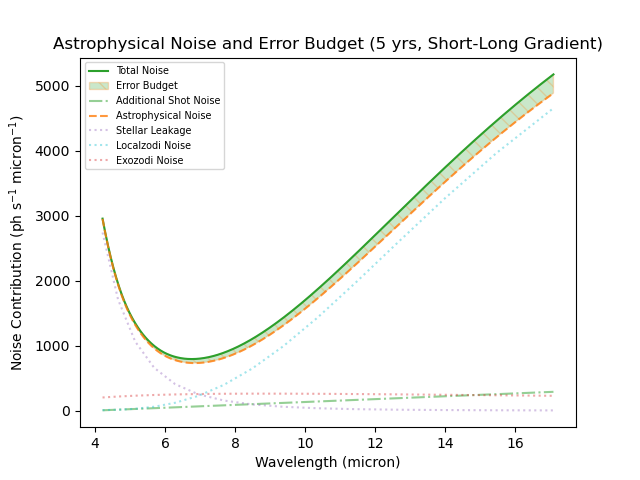
\includegraphics[width=0.8\linewidth]{images/ts reduction/short_long_5yrs.png}
\caption{Depiction of the noise budget on top of the astrophysical noise. The dashed green line denotes the budget distribution, in this case a linear distribution from short to long wavelengths. The solid green line stands for the total noise including the budget. The shaded green area between the astrophysical and total noise curves is the actual error budget. In this example the budget is distributed such that the total mission time is exactly five years.}
\label{fig: budget example}
\end{figure}

\subsection{\DIFdelbegin \DIFdel{Image Size }\DIFdelend \DIFaddbegin \DIFadd{Analytic Background Evaluation }\DIFaddend and Spectral Resolution} \label{sec: ts reduction: image spec}
\DIFdelbegin \DIFdel{Not all quantities that govern the AMS runtime are physical parameters in the sense of Section \ref{sec: intro: params}. Two of them, the }\textit{\DIFdel{image size}} %DIFAUXCMD
\DIFdel{and the }\textit{\DIFdel{spectral resolution}}%DIFAUXCMD
\DIFdel{, are purely numerical settings of the SNR computation. The image size is the side length, in pixels, of the square field-of-view grid on which the exo-zodiacal and local-zodiacal background integrals are evaluated. The spectral resolution is the number of wavelength bins into which the observed spectrum is divided. Both are fixed in the mission itself and are therefore not part of the trade space. However, since the AMS runs its SNR flow over the entire target catalog, and does so repeatedly during trade space exploration, the cost of a single SNRevaluation scales directly with both settings.
It is hence worthwhile to choose the smallest values that do not compromise fidelity, thereby speeding up every subsequent AMS call. This is exactly the type of reduction this chapter is concerned with, applied to the simulator itself rather than to the parameters. }%DIFDELCMD < 

%DIFDELCMD < %%%
\DIFdel{The guiding principle is convergence. As we increase either setting, the computed SNR approaches a limit,
the "true" value that a perfectly resolved simulation would yield. We may therefore treat a very high-resolution run as ground truth and measure, per target, the relative SNR error of a coarser run against it. The smallest setting for which this error has plateaued at a negligible level is the ideal choice: any finer would only cost runtime, any coarser would falsify the result. Crucially, we do not judge convergence by a central value alone. A mean or median error can be driven low simply by averaging many well-sampled targets against a few badly sampled ones, hiding the fact that individual planets are grossly wrong. We therefore track both the mean error and the }\textit{\DIFdel{spread}} %DIFAUXCMD
\DIFdel{of the per-target error across the catalog, }\DIFdelend \DIFaddbegin \DIFadd{The approved physics rewrite removes the science dependence on image size. Circularly symmetric sources permit an analytic azimuthal and radial reduction of the background integrals: the stellar disk is treated as uniform and circular, local zodiacal light as locally uniform, }\DIFaddend and \DIFdelbegin \DIFdel{require both to be small before accepting a setting.
}\DIFdelend \DIFaddbegin \DIFadd{exozodiacal light as smooth and face-on. Inclined or asymmetric exozodiacal disks require an angle-resolved treatment and are outside this reduction. Image size now affects visualization and independent cross-checks only, not production science SNR.
}\DIFaddend 

\DIFdelbegin \DIFdel{We first consider the image size. It only enters the SNR through the background field-of-view integrals; the planetary transmission is evaluated analytically and any instrumental noise floor is independent of the spatial grid. The image size is hence a pure spatial discretization knob with a genuine converged limit. Fig. \ref{fig: image size convergence a} shows, for four regimes of increasing instrumental noise (I/N), the mean relative SNR error against a high-resolution reference of 512 pixels, together with a shaded band spanning the 16th to 84th percentile of the per-target error distribution. The mean settles onto a low plateau at an image size of about 160 pixels, which we adopt. Notably, adding instrumental noise }\textit{\DIFdel{dilutes}} %DIFAUXCMD
\DIFdel{the image-size error rather than aggravating it: the noise floor is spatially independent, so it enlarges the total noise while the spatial sampling error stays fixed. Higher instrumental noise therefore makes the image-size choice }\textit{\DIFdel{less}} %DIFAUXCMD
\DIFdel{critical, which is convenient, since the mission is designed to operate in the background-limited regime where the requirement is at its most stringent. }%DIFDELCMD < 

%DIFDELCMD < \begin{figure}[htbp]
%DIFDELCMD <     \centering
%DIFDELCMD <     \begin{subfigure}{.49\textwidth}
%DIFDELCMD <         \centering
%DIFDELCMD <         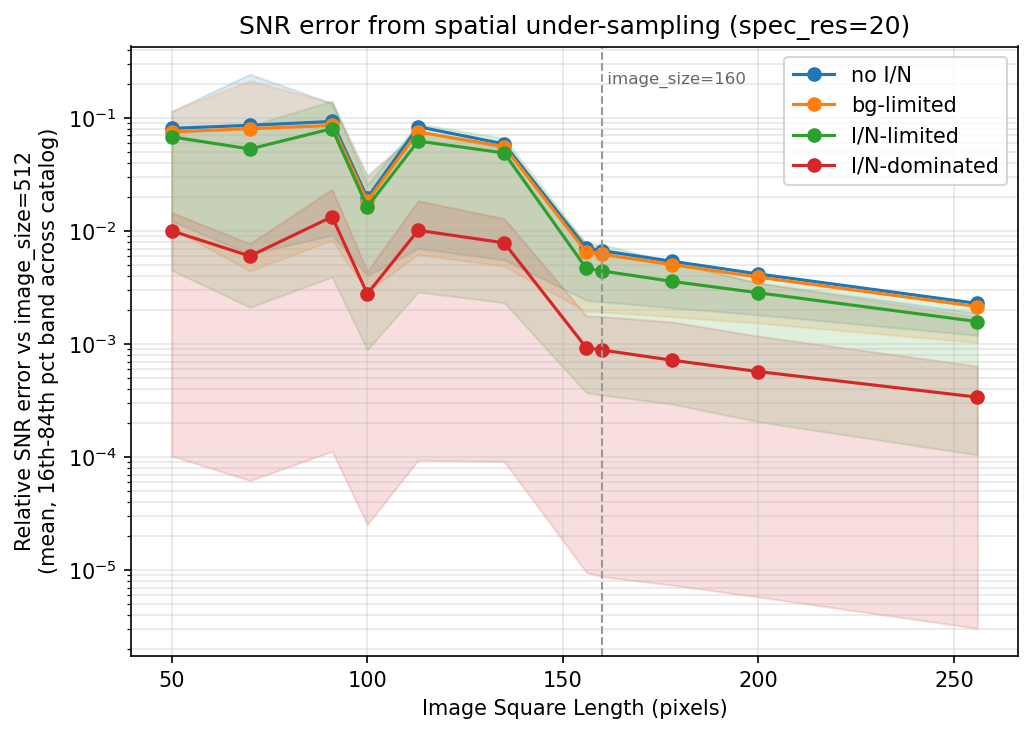
\includegraphics[width=\linewidth]{images/ts reduction/is_error_vs_imagesize.png}
%DIFDELCMD <         %%%
%DIFDELCMD < \caption{%
{%DIFAUXCMD
\DIFdelFL{Convergence and plateau}}
        %DIFAUXCMD
%DIFDELCMD < \label{fig: image size convergence a}
%DIFDELCMD <     \end{subfigure}
%DIFDELCMD <     \begin{subfigure}{.49\textwidth}
%DIFDELCMD <         \centering
%DIFDELCMD <         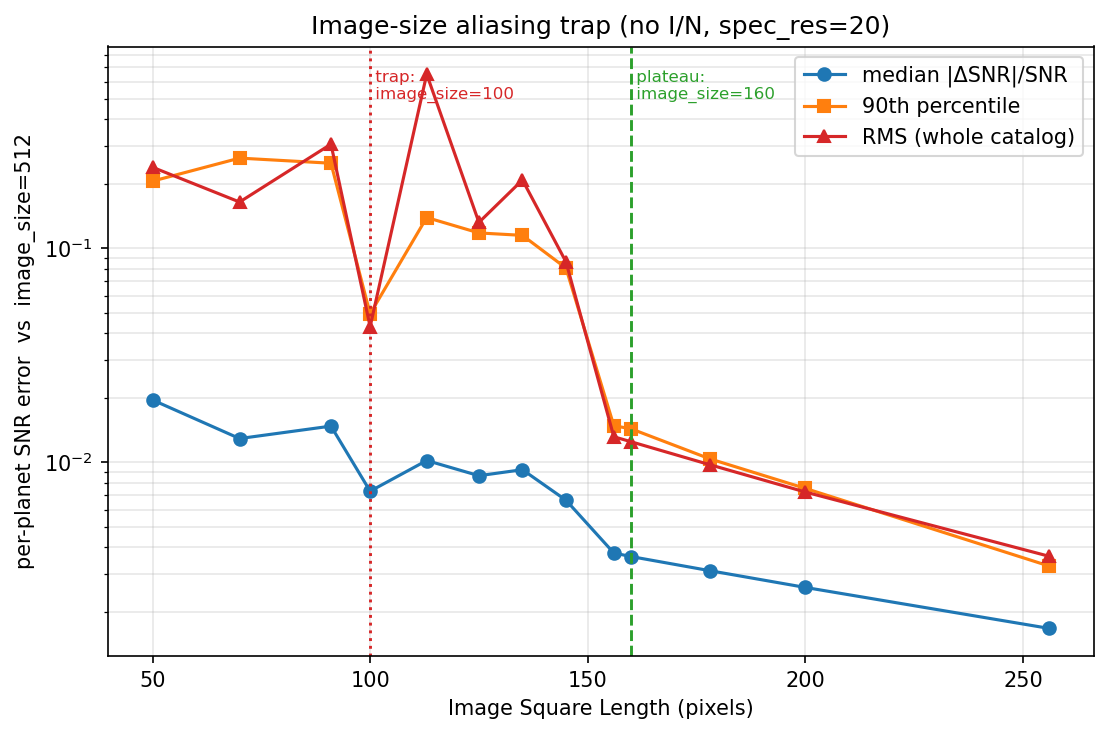
\includegraphics[width=\linewidth]{images/ts reduction/is_aliasing_trap.png}
%DIFDELCMD <         %%%
%DIFDELCMD < \caption{%
{%DIFAUXCMD
\DIFdelFL{The aliasing trap at 100 pixels}}
        %DIFAUXCMD
%DIFDELCMD < \label{fig: image size convergence b}
%DIFDELCMD <     \end{subfigure}
%DIFDELCMD <     %%%
%DIFDELCMD < \caption{%
{%DIFAUXCMD
\DIFdelFL{Image-size convergence of the bulk SNR. (a) Mean relative SNR error against a 512-pixel spatial reference (solid lines), with a shaded band giving the 16th--84th percentile spread across the catalog, for four regimes of increasing instrumental noise (I/N). Both the mean and the spread plateau around an image size of 160 pixels (dashed line); below it the band is very wide, showing that many individual targets are badly mis-sampled even where the mean is only moderate. Additional instrumental noise pushes the curves lower, confirming that the background-limited regime is the most demanding. (b) A cautionary detail. At an image size of 100 pixels the median, the 90th percentile, and the whole-catalog RMS all dip to a local minimum together, so the error looks small by every statistic. This is a coincidental aliasing cancellation, not convergence: the immediate neighbours spike (the whole-catalog RMS reaches nearly 60\% at 113 pixels), the minimum is razor-thin, and even the dip stays several times above the genuine plateau. Robust convergence, low and stable against small changes in the grid, begins only near 160 pixels.}}
    %DIFAUXCMD
%DIFDELCMD < \label{fig: image size convergence}
%DIFDELCMD < \end{figure}
%DIFDELCMD < 

%DIFDELCMD < %%%
\DIFdel{The spread is what turns this from a plausible choice into a firm one. Below roughly 156 pixels the 16th--84th percentile band in Fig. \ref{fig: image size convergence a} is generally very wide (with one deceptive exception at 100 pixels, discussed below): individual targets scatter to several tens of percent relative error even where the mean sits near ten percent. In other words, the catalog average looks merely mediocre while a large fraction of planets are in fact grossly mis-sampled. At 156--160 pixels the band collapses together with the mean , which is the true signature of convergence: not only the average but }\textit{\DIFdel{every}} %DIFAUXCMD
\DIFdel{target is now well sampled. This is precisely the distinction a central value alone cannot make}\DIFdelend \DIFaddbegin \DIFadd{The reduction follows from expanding the even power $\sin^{2p}\phi$ into cosines. Azimuthal averaging then uses the standard Bessel integral representation \mbox{%DIFAUXCMD
\cite{nistdlmf}}\hskip0pt%DIFAUXCMD
,
}\begin{align}
\DIFadd{\frac{1}{2\pi}\int_0^{2\pi}\cos(z\cos\varphi)\,\mathrm{d}\varphi=J_0(z).
}\end{align}
\DIFadd{For null order $n=2p$, azimuthally averaging one destructive output at angular radius $\vartheta$ gives
}\begin{align}
\DIFadd{\left\langle T_{2p}\right\rangle_\varphi(\vartheta)
}&\DIFadd{=
\frac{1}{2}\frac{\binom{2p}{p}}{4^p}
+\sum_{j=1}^{p}(-1)^j\frac{\binom{2p}{p-j}}{4^p}
J_0\left(\frac{2\pi j b\vartheta}{\lambda}\right).
\label{eq: general null average}
}\end{align}
\DIFadd{For a uniform disk, radial area averaging replaces each $J_0(jx)$ term by $2J_1(jx)/(jx)$, following the standard Bessel derivative identity \mbox{%DIFAUXCMD
\cite{nistdlmf}}\hskip0pt%DIFAUXCMD
, where $x=2\pi bR/\lambda$ and $R$ is the angular disk radius. The limiting value is one as $jx\rightarrow0$, so the expression is evaluated with its analytic limit near the origin. The Bessel power series then gives the small-star limits
}\begin{align}
\DIFadd{\left\langle T_2\right\rangle_\mathrm{disk}
}&\DIFadd{=\frac{x^2}{32}+\mathcal{O}(x^4),}\\
\DIFadd{\left\langle T_4\right\rangle_\mathrm{disk}
}&\DIFadd{=\frac{x^4}{256}+\mathcal{O}(x^6).
\label{eq: leakage small star}
}\end{align}
\DIFadd{The fourth-to-second-order stellar-leakage ratio therefore approaches $x^2/8$. The same general average is used inside one-dimensional radial quadrature for a tapered source or exozodiacal profile. Rotation does not ``average away'' a circular background; rather, circular symmetry makes its integrated response independent of rotation angle. Its mean may cancel after chopping, but its photons still set the shot-noise variance}\DIFaddend .

\DIFdelbegin \DIFdel{A second, more treacherous pitfall appears around an image size of 100 pixels. As Fig. \ref{fig: image size convergence b} shows, the error dips to a local minimum there, and not just in the median: the 90th percentile and the whole-catalog RMS dip in lockstep, so at that one grid size the error looks small by every statistic. The dip is nonetheless spurious. It is a coincidental aliasing cancellation, at that exact pixel pitch the disk-mask sampling error happens to cancel across the catalog, rather than the grid having genuinely resolved the disks. The giveaway is its fragility: the immediate neighbours explode, with the whole-catalog RMS leaping to nearly 60\% at an image size of 113 pixels, and even the dip itself, at roughly 5\%, remains several times worse than the true plateau of about 1.3\% at 160 pixels. A converged setting must be low }\textit{\DIFdel{and}} %DIFAUXCMD
\DIFdel{stable against small changes in the grid; the 100-pixel notch is instead a razor-thin minimum surrounded by maxima, the very opposite of convergence, and it would shift or vanish for a different catalog or resolution. Genuine, robust convergence sets in only from around 160 pixels, which is why we accept that plateau and not the coincidental dip}\DIFdelend \DIFaddbegin \DIFadd{The local-zodiacal correction arose from a geometric inconsistency in the removed pixel-grid path. The physical field of view is circular, with solid angle proportional to $\pi R_\mathrm{FoV}^2$, but one normalization divided the integrated circular flux by the area $4R_\mathrm{FoV}^2$ of its enclosing square. It therefore suppressed the uniform foreground by $\pi/4$. Restoring the circular normalization multiplies the local-zodiacal rate by
}\begin{align}
\DIFadd{\frac{4}{\pi}=1.2732\ldots,
}\end{align}
\DIFadd{an increase of approximately 27.3\%}\DIFaddend . \DIFaddbegin \DIFadd{This is a normalization correction, not a new dust model. Because local-zodiacal shot noise is present for every target, the change propagates nonlinearly through SNR, target ranking, and the 90th-percentile mission time.
}\DIFaddend 

\DIFdelbegin \DIFdel{We turn to the spectral resolution. Here the situation is qualitatively different, and in fact more forgiving. The bulk SNR combines the per-bin contributions as $\text{SNR}_\text{tot} = \sqrt{\sum_i \text{SNR}_{\lambda_i}^2}$ (eq. \ref{eq: bulk snr}). Whenever the noise is purely photon- or background-limited, this sum is invariant under the choice of binning: splitting a bin in two divides both its signal and its noise consistently, leaving the quadrature sum unchanged. Since the baseline instrument carries no per-channel detector floor, the spectral resolution is essentially irrelevant to the yield, and a coarse resolution of 20 bins is numerically indistinguishable from a fully resolved run. Fig. \ref{fig: spec res convergence} confirms this: in the no-I/N and background-limited regimes the mean relative error at a spectral resolution of 20 is already at the $10^{-4}$ level, and, just as importantly, its 16th--84th percentile band is equally tight, so no individual target is poorly resolved either. The resolution only begins to matter once a per-channel floor is switched on, because such a floor does not scale with the bin width; then finer binning spreads a fixed noise floor across more channels and both the mean error and its spread at low resolution grow. Since we operate in the background-limited regime, a spectral resolution of 20 is amply sufficient, and we adopt it. }%DIFDELCMD < 

%DIFDELCMD < \begin{figure}[htbp]
%DIFDELCMD <     \centering
%DIFDELCMD <     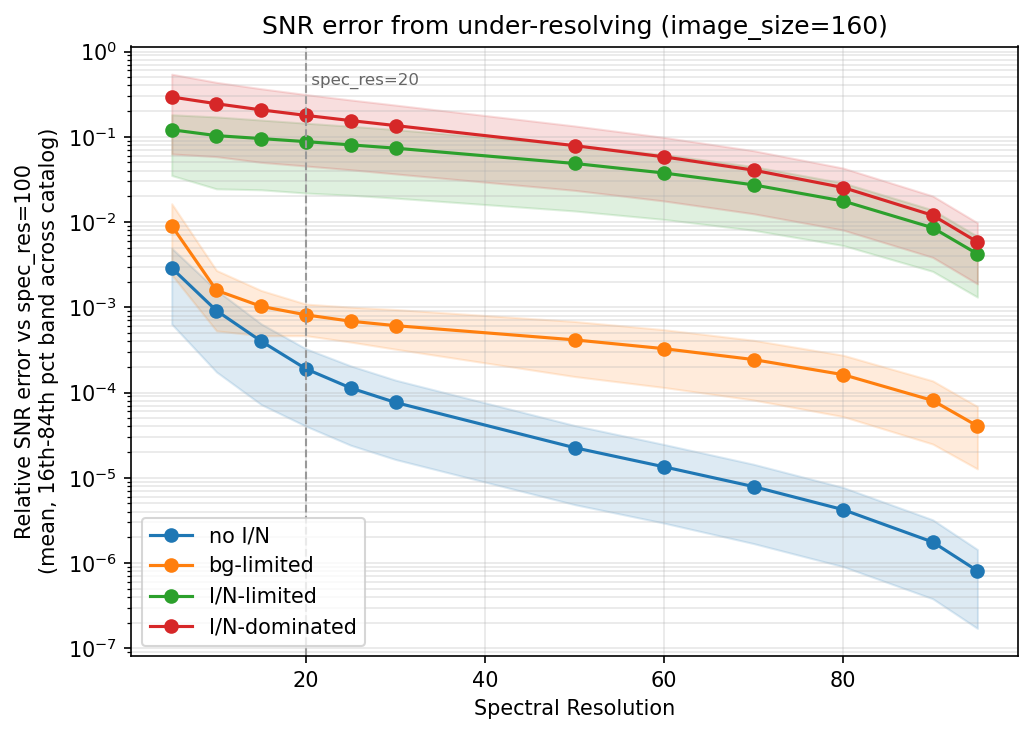
\includegraphics[width=0.7\linewidth]{images/ts reduction/sr_error_vs_specres.png}
%DIFDELCMD <     %%%
%DIFDELCMD < \caption{%
{%DIFAUXCMD
\DIFdelFL{Spectral-resolution sensitivity of the bulk SNR. The mean relative SNR error against a fully resolved reference of 100 bins (solid lines), with a shaded 16th--84th percentile band across the catalog, is plotted against the spectral resolution for the same four instrument-noise regimes. In the no-I/N and background-limited regimes (the mission's operating point), both the mean and the band at a spectral resolution of 20 (dashed line) are already negligible, confirming that the quadrature-combined SNR is essentially resolution-invariant for every target, not just on average. Only when a per-channel detector floor is switched on, which does not scale with bin width, does the coarse resolution incur a sizeable error, motivating why the setting can safely be minimized for our purposes.}}
    %DIFAUXCMD
%DIFDELCMD < \label{fig: spec res convergence}
%DIFDELCMD < \end{figure}
%DIFDELCMD < 

%DIFDELCMD < %%%
\DIFdel{In summary, we fix the AMS SNR computation to an image size of 160 pixels and a spectral resolution of 20 bins. These are the smallest values that reach the converged plateau in the regime the mission operates in , minimizing the runtime of every AMS evaluation without measurably degrading the yield}\DIFdelend \DIFaddbegin \DIFadd{Transmission and source spectra are integrated within every wavelength bin using an eight-point Gauss--Legendre rule in inverse wavelength $u=1/\lambda$. This coordinate is natural because interferometric phases are proportional to $b/\lambda$ and therefore vary nearly linearly with $u$. Across spectral resolutions 5, 10, 20, and 50 and sampled catalog stars, the stellar-leakage and exozodiacal terms agree with a 64-point reference to approximately machine precision. The adopted resolving power remains $R=\lambda/\Delta\lambda=20$, which produces 31 bins over 4--18.5\,$\upmu$m. Thus spatial image size is no longer a science parameter, while wavelength-bin integration is explicitly converged for the retained binning. Appendix \ref{app: analytic derivation} records the derivation and numerical conventions in greater detail}\DIFaddend .

\subsection{Restriction of Null Order}
\DIFdelbegin \DIFdel{We described a composite approach to null order simulation }\DIFdelend \DIFaddbegin \DIFadd{The proxy described }\DIFaddend in Section \ref{sec: intro: null depth approach} \DIFdelbegin \DIFdel{. The corresponding transmission maps allow for any integer value of null order $n$. In practice, the geometry of the interferometer and the corresponding transmission maps only allow for }\DIFdelend \DIFaddbegin \DIFadd{accepts positive }\DIFaddend even null orders. \DIFdelbegin \DIFdel{Since the double Bracewell interferometer has a null order of two, we may only additionally consider null orders 2, 4, 6, ... An instrument with a higher null order needs more mixing of constructive and destructive outputs, which increases the number of required instrument apertures. A null order of six already requires a minimum of eight (TODO: verify??? CITE) apertures which will almost certainly not be operationally realizable. We hence have a natural focus on the null orders of }\DIFdelend \DIFaddbegin \DIFadd{This thesis evaluates null orders }\DIFaddend two and four. \DIFdelbegin \DIFdel{Since building an instrument with a null order of four already requires at least two more apertures(TODO: verify???, CITE), even considering such an architecture would undoubtedly require much stronger performance compared to the currently envisioned second order null}\DIFdelend \DIFaddbegin \DIFadd{Order two reproduces the double-Bracewell null envelope; order four is a controlled mathematical proxy using the same four apertures, collecting area, efficiency, baseline ratio, and per-target baseline prescription. No aperture-count or hardware-feasibility claim follows from the fourth-order calculation}\DIFaddend .

\DIFdelbegin \section{\DIFdel{Trade Space Exploration}} %DIFAUXCMD
\addtocounter{section}{-1}%DIFAUXCMD
\DIFdelend \DIFaddbegin \chapteropening{Trade Space Exploration}{From the reduced parameter space to an iso-mission-time random-noise allowance} \DIFaddend \label{sec: tse}
With the trade space reduced\DIFdelbegin \DIFdel{to an interpretable size, we can finally address the inverse problem posed in Section \ref{sec: intro: trade space}: for a given target mission time, how much random-noise budget can the instrument afford, and how does that budget depend on its distribution over wavelength and on the agnostic operating point? This section presents a first exploration of the reduced trade space. All results reported here are computed for a null order of two, i.e. the nominal double Bracewell architecture. The corresponding exploration for higher null orders , and the architecture comparison it enables, is left as future work (see Section \ref{sec: tse: null order})}\DIFdelend \DIFaddbegin \DIFadd{, we now invert the AMS mapping. All results use the approved analytic background model and a deliberately conservative common operating point unless a plotted axis varies it. The working LIFE field-of-regard reference is $90^\circ$; $65^\circ$ is substantially more restrictive but still permits acceptable mission times. Current project estimates place the K-band limiting magnitude near 8; magnitude 7 is a pessimistic lower bound, and the completed scans show little remaining sensitivity near that value. A 10\,h slew is the inherited baseline \mbox{%DIFAUXCMD
\cite{dannert2025thesis}}\hskip0pt%DIFAUXCMD
; 12\,h adds an intentionally simple 20\% margin, while longer slews rapidly remove feasible budget space. The choices are therefore conservative comparison points, not optimized requirements. Hab2Max is evaluated at study targets of 5.5 and 6\,yr; Hab2Min uses 7.5 and 8\,yr. Both null orders use the same source catalogs and assumptions}\DIFaddend .

\subsection{The Iso-Mission-Time Budget}
The \DIFdelbegin \DIFdel{quantity we solve for is the }\textit{\DIFdel{iso-mission-time budget}}%DIFAUXCMD
\DIFdel{: the largest additive instrumental noise term }\DIFdelend \DIFaddbegin \textit{\DIFadd{iso-mission-time budget}} \DIFadd{is the tolerated scalar amplitude of one imposed }\DIFaddend $N_I(\lambda)$ \DIFdelbegin \DIFdel{(Section \ref{sec: ts reduction: condensation}) that can be added on top of the astrophysical noise while the required mission time still equals a chosen target}\DIFdelend \DIFaddbegin \DIFadd{shape at a stated operating point}\DIFaddend . It is expressed \DIFdelbegin \DIFdel{as a photon flux density }\DIFdelend in ph\,s$^{-1}$\,$\upmu$m$^{-1}$ \DIFdelbegin \DIFdel{and represents, for that operating point, the error budget in the sense of this thesis: any instrument whose random noise stays below it completes the mission in the target time}\DIFdelend \DIFaddbegin \DIFadd{for the flat case or as a ramp endpoint. ``Below'' applies only to the same imposed shape and reference calculation}\DIFaddend .

\DIFdelbegin \DIFdel{Locating this budget for any set functional budget form efficiently exploits the monotonicity established in Section \ref{sec: intro: trade space}: since the mission time increases monotonically as budget is added,the budget at which it reaches a given target is unique. Empirically the mission time grows roughly exponentially with the budget, so the search fits a function $m(\text{budget}) = a\,e^{b\,\text{budget}}$ through the mission times at the current bracketing bounds, inverts it to predict the budget at the target time, evaluates the AMS there, and tightens whichever bound the prediction lies closest to. The procedure repeats until the mission time is within $0.05$ years }\DIFdelend \DIFaddbegin \DIFadd{The search starts with an amplitude bracket from 0 to 50,000 ph\,s$^{-1}$\,$\upmu$m$^{-1}$. At every iteration the lower bracket endpoint is admissible and the upper endpoint exceeds the target mission time. An exponential fit through the endpoint evaluations proposes the next amplitude; it accelerates the search but does not define the answer. The new evaluation replaces one endpoint according to its mission time, so the bracket invariant is retained. The search stops when mission time lies within 0.05\,yr }\DIFaddend of the target or the \DIFdelbegin \DIFdel{bracket has collapsed. Two outcomes carry physical meaning: if the mission time already exceeds the target at zero added budget, the target is unreachable and no extra noise is permissible (a budget of zero); if it is met even at the largest tested budget, that bound is returned}\DIFdelend \DIFaddbegin \DIFadd{amplitude bracket is at most 10\,ph\,s$^{-1}$\,$\upmu$m$^{-1}$ wide. Reported amplitudes are therefore search point estimates. The two alternative stopping rules do not support a universal $\pm5$ amplitude uncertainty: a time-tolerance stop may leave a wider amplitude bracket, whereas a bracket-width stop only bounds the final numerical search interval.
}

\DIFadd{Within a fixed target list, added independent variance can only lower individual SNRs. The full mission-time map also includes discrete rankings and a sampled percentile, so global monotonicity is an empirical property rather than a formal theorem. The completed scans showed nested contours and no folded iso-time branches at the sampled resolution. If the zero-budget calculation already exceeds the requested time, no non-negative allowance exists; the plotted dark region represents this physically infeasible operating point, not a failed numerical search}\DIFaddend .

\subsection{The Shape of the Error Budget}
The first question is how the affordable budget depends on its \textit{distribution} over wavelength. We compare three \DIFdelbegin \DIFdel{shapes at a fixed operating point (limiting magnitude 7, field of regard $65^\circ$, slew time 12\,h) for the Hab2Max catalog:
a flat budget, a budget ramped linearly from zero at the short-wavelength end to a maximum at the long-wavelength end (matching the exo- and local-zodiacal noise, which dominate the long wavelengths), and the opposite ramp peaking at short wavelengths (matching the stellar leakage, which dominates the short wavelengths). Figure \ref{fig: tse budget shapes} shows the three cases directly, each tuned so that the required mission time is exactly five years. In every panel the astrophysical noise forms the familiar U-shape: high at short wavelengths where the stellar leakage dominates, high again at long wavelengths where the local- and exo-zodiacal emission take over, and reaching a minimum near 7\,$\upmu$m. The added budget $N_I$ is laid on top of this, and }\DIFdelend \DIFaddbegin \DIFadd{one-parameter families:
}\begin{align}
\DIFadd{N_\mathrm{flat}(\lambda)}&\DIFadd{=A,}\\
\DIFadd{N_\mathrm{short}(\lambda)}&\DIFadd{=A\,\frac{18.5\,\upmu\mathrm{m}-\lambda}{14.5\,\upmu\mathrm{m}},}\\
\DIFadd{N_\mathrm{long}(\lambda)}&\DIFadd{=A\,\frac{\lambda-4\,\upmu\mathrm{m}}{14.5\,\upmu\mathrm{m}}.
}\end{align}
\DIFadd{Here $A$ is }\DIFaddend the \DIFdelbegin \DIFdel{shaded band between the astrophysical and total noise is the error budget itself.
The three panels differ only in how that budget is distributed across the spectrum. The endpoints at which each shape reaches the five-year target are listed in Table \ref{tab: budget shapes}.
}\DIFdelend \DIFaddbegin \DIFadd{reported amplitude. The ramp endpoints are imposed shape parameters, not independently inferred wavelength limits. Figures \ref{fig: tse budget shapes no2} and \ref{fig: tse budget shapes no4} show the Hab2Max 5.5-year solutions.
}\DIFaddend 

\begin{figure}[htbp]
    \centering
    \begin{subfigure}{.32\textwidth}
        \centering
        \DIFdelbeginFL %DIFDELCMD < 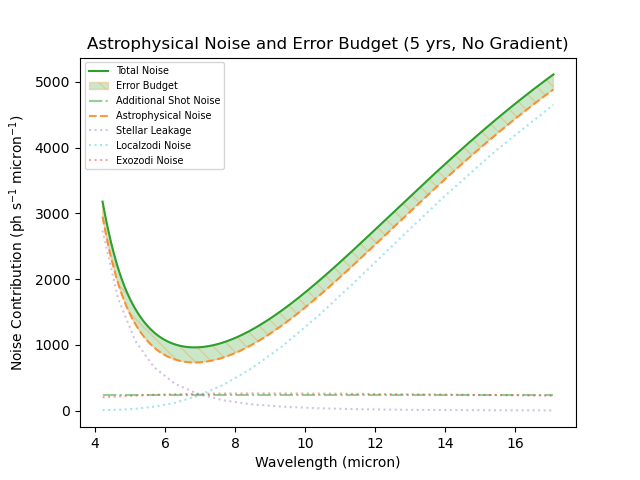
\includegraphics[width=\linewidth]{images/tse/tse_budget_constant_5yr.png}
%DIFDELCMD <         %%%
\DIFdelendFL \DIFaddbeginFL 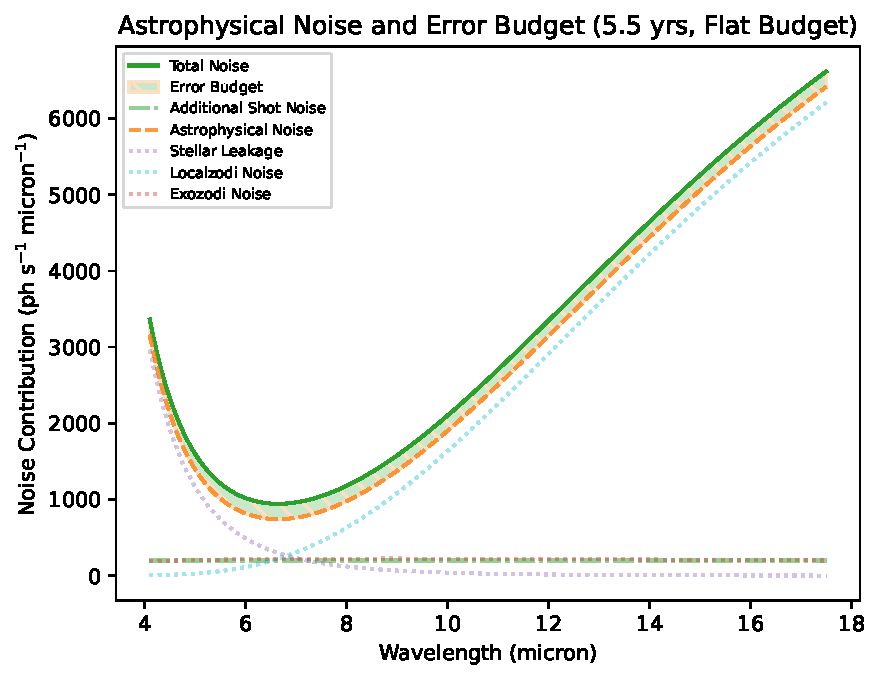
\includegraphics[width=\linewidth]{images/tse/final/no2_hi_flat_5p5.pdf}
        \DIFaddendFL \caption{Flat}
    \DIFdelbeginFL %DIFDELCMD < \label{fig: tse budget shapes a}
%DIFDELCMD <     %%%
\DIFdelendFL \end{subfigure}
    \begin{subfigure}{.32\textwidth}
        \centering
        \DIFdelbeginFL %DIFDELCMD < 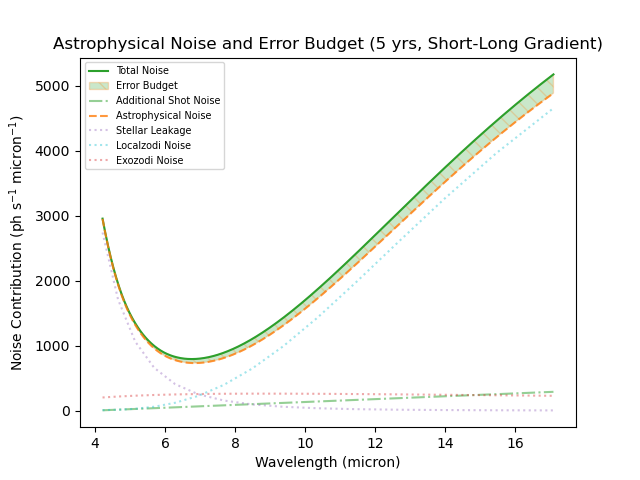
\includegraphics[width=\linewidth]{images/tse/tse_budget_shortlong_5yr.png}
%DIFDELCMD <         %%%
\DIFdelendFL \DIFaddbeginFL 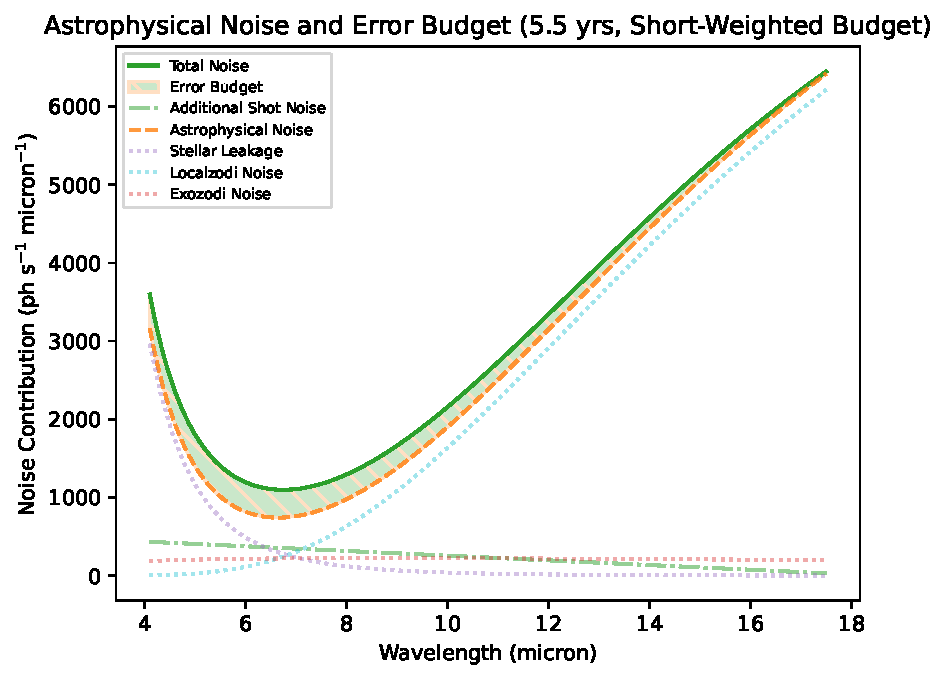
\includegraphics[width=\linewidth]{images/tse/final/no2_hi_short_5p5.pdf}
        \caption{\DIFaddFL{Short-weighted}}
    \end{subfigure}
    \begin{subfigure}{.32\textwidth}
        \centering
        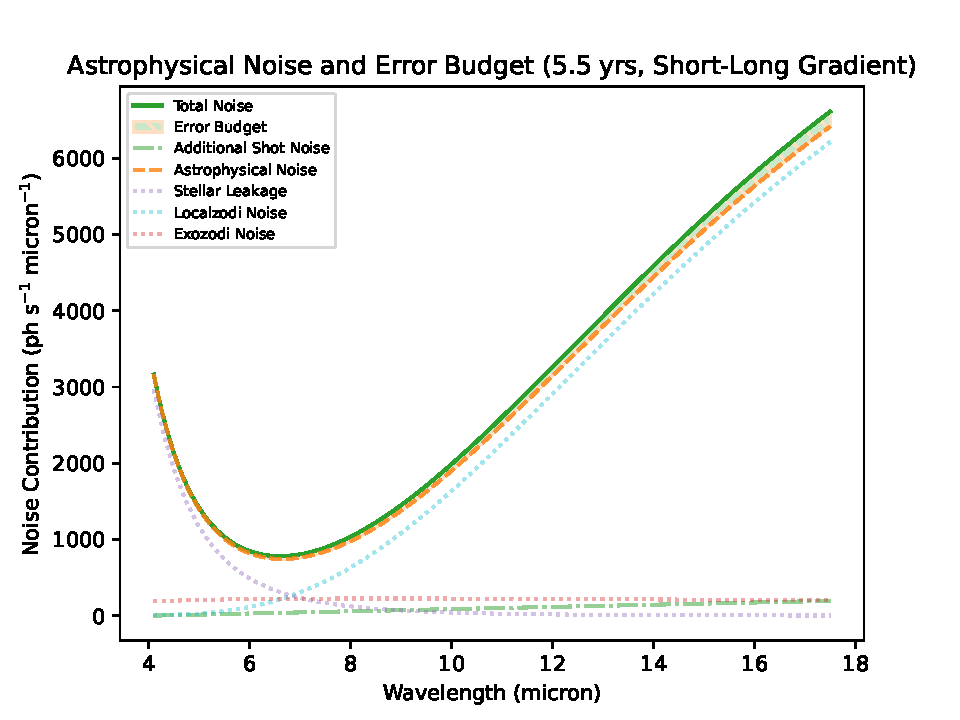
\includegraphics[width=\linewidth]{images/tse/final/no2_hi_long_5p5.pdf}
        \DIFaddendFL \caption{Long-weighted}
    \DIFdelbeginFL %DIFDELCMD < \label{fig: tse budget shapes b}
%DIFDELCMD <     %%%
\DIFdelendFL \end{subfigure}
    \DIFaddbeginFL \caption{\DIFaddFL{Final null-order-two Hab2Max budgets at the common operating point and 5.5-year target. Stellar leakage dominates the short-wave astrophysical background, so the short-weighted ramp admits the largest endpoint.}}
    \label{fig: tse budget shapes no2}
\end{figure}

\begin{figure}[htbp]
    \centering
    \DIFaddendFL \begin{subfigure}{.32\textwidth}
        \centering
        \DIFdelbeginFL %DIFDELCMD < 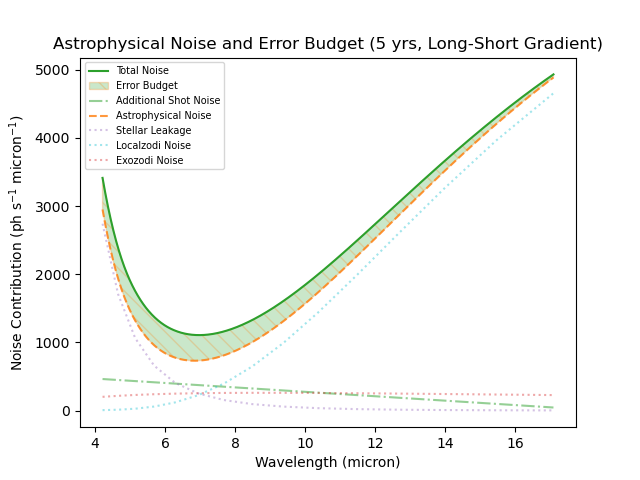
\includegraphics[width=\linewidth]{images/tse/tse_budget_longshort_5yr.png}
%DIFDELCMD <         %%%
\DIFdelendFL \DIFaddbeginFL 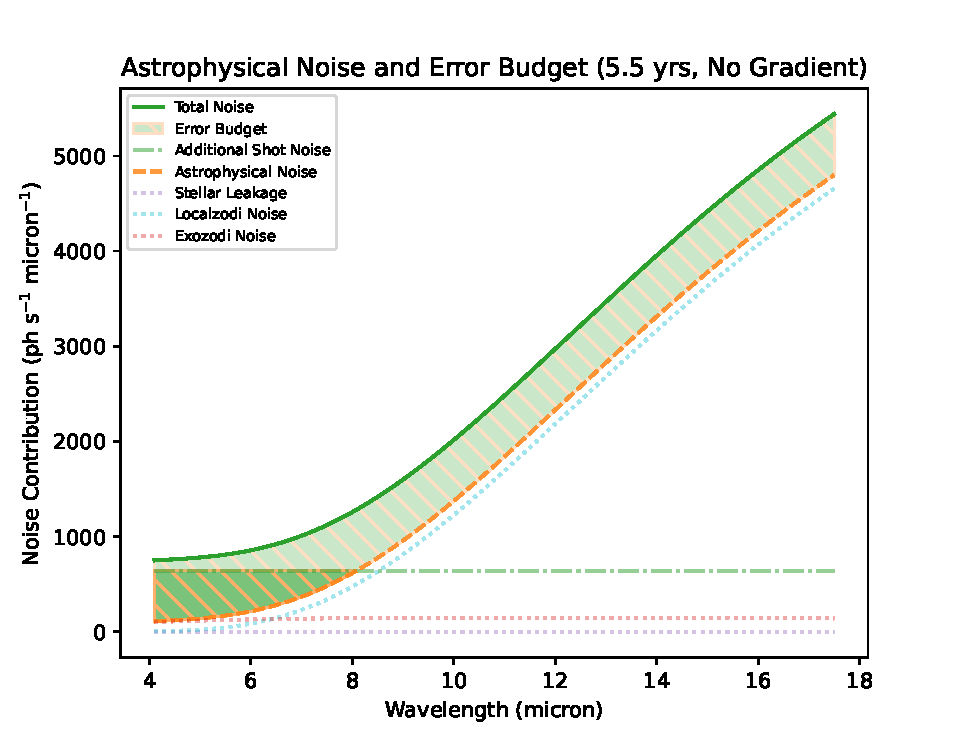
\includegraphics[width=\linewidth]{images/tse/final/no4_hi_flat_5p5.pdf}
        \caption{\DIFaddFL{Flat}}
    \end{subfigure}
    \begin{subfigure}{.32\textwidth}
        \centering
        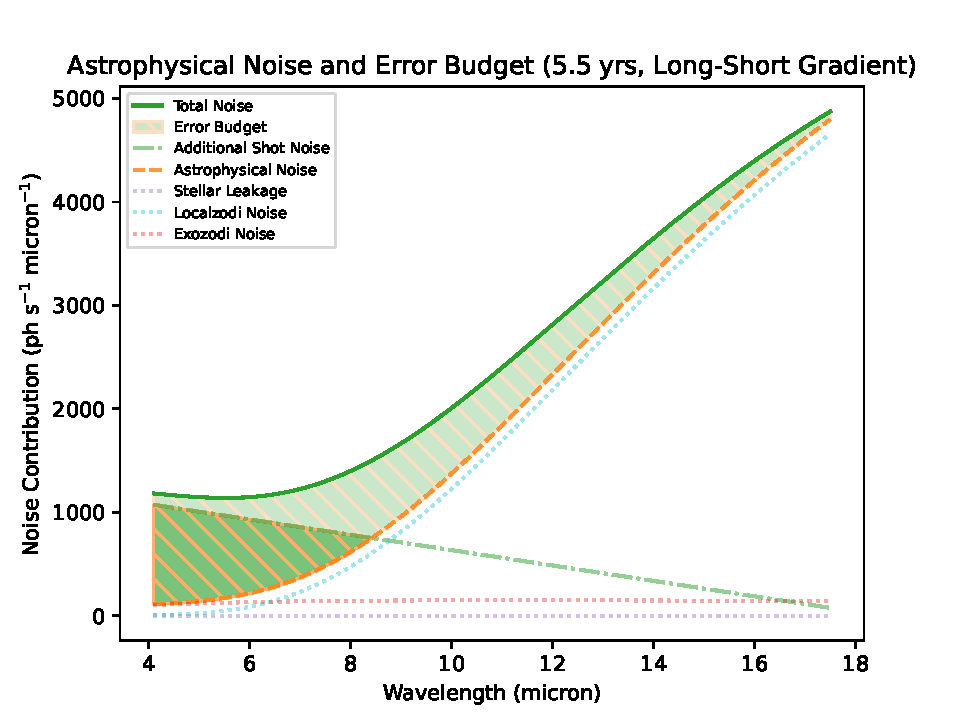
\includegraphics[width=\linewidth]{images/tse/final/no4_hi_short_5p5.pdf}
        \DIFaddendFL \caption{Short-weighted}
    \DIFdelbeginFL %DIFDELCMD < \label{fig: tse budget shapes c}
%DIFDELCMD <     %%%
\DIFdelendFL \end{subfigure}
    \DIFaddbeginFL \begin{subfigure}{.32\textwidth}
        \centering
        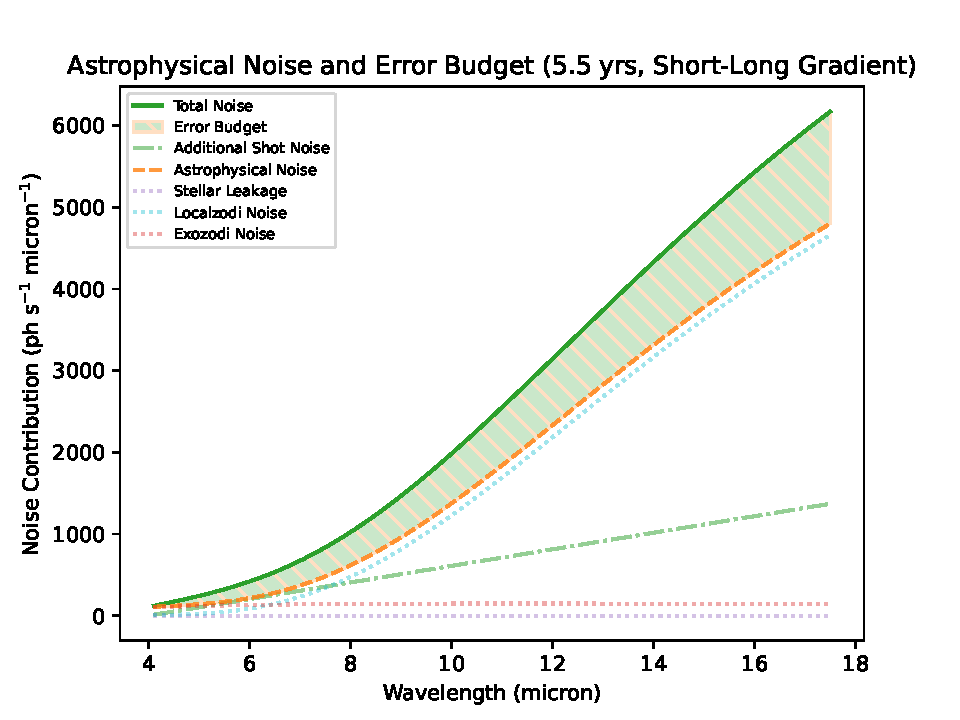
\includegraphics[width=\linewidth]{images/tse/final/no4_hi_long_5p5.pdf}
        \DIFaddendFL \caption{\DIFdelbeginFL \DIFdelFL{The random-noise error budget laid on top of the astrophysical noise, for the Hab2Max catalog at a limiting magnitude of 7, a field of regard of $65^\circ$ and a slew time of 12\,h, with a null order of two. Each panel is tuned so that the required mission time is exactly five years. The orange dashed curve is the astrophysical noise, the green solid curve the total noise, and the green shaded band between them the error budget, i.e. the added noise $N_I$; the dotted curves are the individual astrophysical sources (stellar leakage, local- and exo-zodiacal). (a) A flat budget of 230 ph\,s$^{-1}$}%DIFDELCMD < {}%%%
\DIFdelFL{$\upmu$m$^{-1}$ across the spectrum. (b) A budget ramped toward the long wavelengths, following the zodiacal emission, reaching 320 at the long end and zero at the short end. (c) A budget ramped toward the short wavelengths, following the stellar leakage, reaching 470 at the short end. The short-weighted shape admits the largest budget, confirming that added noise is least costly where the stellar leakage already dominates.}\DIFdelendFL \DIFaddbeginFL \DIFaddFL{Long-weighted}\DIFaddendFL }
    \DIFdelbeginFL %DIFDELCMD < \label{fig: tse budget shapes}
%DIFDELCMD < %%%
\DIFdelendFL \DIFaddbeginFL \end{subfigure}
    \caption{\DIFaddFL{Final null-order-four proxy budgets for the same Hab2Max operating point and target as Fig. \ref{fig: tse budget shapes no2}. Geometric stellar leakage is nearly absent. The long-weighted ramp now admits the largest endpoint because the remaining background is dominated by zodiacal emission toward long wavelengths.}}
    \label{fig: tse budget shapes no4}
\DIFaddendFL \end{figure}

\begin{table}[htbp]
\centering
\DIFdelbeginFL %DIFDELCMD < \begin{tabular}{@{}llccc@{}}
%DIFDELCMD < %%%
\DIFdelendFL \begin{tabular}{@{}llrrrr@{}}
\toprule
Catalog & MT target & \DIFaddbeginFL \DIFaddFL{Null order }& \DIFaddendFL Flat & Short-weighted & Long-weighted \\
        & \DIFaddFL{[yr]} & & \multicolumn{3}{c}{\DIFaddFL{Amplitude }[\DIFaddFL{ph\,s$^{-1}$\,$\upmu$m$^{-1}$}]} \\
\midrule
Hab2Max & \DIFdelbeginFL \DIFdelFL{5 yr  }\DIFdelendFL \DIFaddbeginFL \DIFaddFL{5.5 }\DIFaddendFL & \DIFdelbeginFL \DIFdelFL{230  }\DIFdelendFL \DIFaddbeginFL \DIFaddFL{2 }\DIFaddendFL & \DIFdelbeginFL \DIFdelFL{470 }\DIFdelendFL \DIFaddbeginFL \DIFaddFL{140 }\DIFaddendFL & \DIFdelbeginFL \DIFdelFL{320 }\DIFdelendFL \DIFaddbeginFL \DIFaddFL{300  }& \DIFaddFL{210  }\DIFaddendFL \\
Hab2Max & \DIFdelbeginFL \DIFdelFL{6 yr  }\DIFdelendFL \DIFaddbeginFL \DIFaddFL{5.5 }\DIFaddendFL & \DIFdelbeginFL \DIFdelFL{1190 }\DIFdelendFL \DIFaddbeginFL \DIFaddFL{4 }\DIFaddendFL & \DIFdelbeginFL \DIFdelFL{3300 }\DIFdelendFL \DIFaddbeginFL \DIFaddFL{650 }\DIFaddendFL & \DIFdelbeginFL \DIFdelFL{2270 }\DIFdelendFL \DIFaddbeginFL \DIFaddFL{1080 }& \DIFaddFL{1470 }\DIFaddendFL \\
\DIFdelFL{Hab2Min }\DIFdelendFL \DIFaddbeginFL \DIFaddFL{Hab2Max }\DIFaddendFL & \DIFdelbeginFL \DIFdelFL{10 yr }\DIFdelendFL \DIFaddbeginFL \DIFaddFL{6.0 }\DIFaddendFL & \DIFdelbeginFL \DIFdelFL{180  }\DIFdelendFL \DIFaddbeginFL \DIFaddFL{2 }\DIFaddendFL & 610 & \DIFdelbeginFL \DIFdelFL{335 }\DIFdelendFL \DIFaddbeginFL \DIFaddFL{1300 }& \DIFaddFL{1090 }\DIFaddendFL \\
\DIFaddFL{Hab2Max }& \DIFaddFL{6.0 }& \DIFaddFL{4 }& \DIFaddFL{940 }& \DIFaddFL{1830 }& \DIFaddFL{2240 }\\
\DIFaddFL{Hab2Min }& \DIFaddFL{7.5 }& \DIFaddFL{2 }& \DIFaddFL{65  }& \DIFaddFL{200  }& \DIFaddFL{150  }\\
\DIFaddFL{Hab2Min }& \DIFaddFL{7.5 }& \DIFaddFL{4 }& \DIFaddFL{590 }& \DIFaddFL{1000 }& \DIFaddFL{1260 }\\
\DIFaddFL{Hab2Min }& \DIFaddFL{8.0 }& \DIFaddFL{2 }& \DIFaddFL{460 }& \DIFaddFL{970  }& \DIFaddFL{810  }\\
\DIFaddFL{Hab2Min }& \DIFaddFL{8.0 }& \DIFaddFL{4 }& \DIFaddFL{790 }& \DIFaddFL{1460 }& \DIFaddFL{1860 }\\
\bottomrule
\end{tabular}
\caption{\DIFdelbeginFL \DIFdelFL{Iso-mission-time additive leakage budgets for three wavelength distributions. For }\DIFdelendFL \DIFaddbeginFL \DIFaddFL{Final amplitudes at }\DIFaddendFL the \DIFdelbeginFL \DIFdelFL{ramped shapes the }\DIFdelendFL \DIFaddbeginFL \DIFaddFL{common operating point. A ramp }\DIFaddendFL value \DIFdelbeginFL \DIFdelFL{quoted }\DIFdelendFL is \DIFdelbeginFL \DIFdelFL{the }\DIFdelendFL \DIFaddbeginFL \DIFaddFL{its }\DIFaddendFL non-zero \DIFaddbeginFL \DIFaddFL{imposed }\DIFaddendFL endpoint\DIFdelbeginFL \DIFdelFL{(the ramp runs linearly to zero at the opposite end)}\DIFdelendFL . \DIFdelbeginFL \DIFdelFL{The Hab2Max rows assume a limiting magnitude of 7, a field of regard of $65^\circ$ and a slew time of 12\,h; }\DIFdelendFL \DIFaddbeginFL \DIFaddFL{These endpoint parameters compare sensitivity within }\DIFaddendFL the \DIFdelbeginFL \DIFdelFL{Hab2Min row assumes a limiting magnitude of 5.25 and a field of regard of $60^\circ$. Values }\DIFdelendFL \DIFaddbeginFL \DIFaddFL{tested families; they }\DIFaddendFL are \DIFdelbeginFL \DIFdelFL{read from the exploration output}\DIFdelendFL \DIFaddbeginFL \DIFaddFL{not common integrated-noise measures or engineering-cost rankings}\DIFaddendFL .}
\label{tab: budget shapes}
\end{table}

\DIFdelbegin \DIFdel{Two robust observations follow. First, the budget grows steeply, and clearly super-linearly, with the permitted mission time : for Hab2Max the flat budget rises from 230 to 1190 ph\,s$^{-1}$}%DIFDELCMD < {}%%%
\DIFdel{$\upmu$m$^{-1}$ between the five- and six-year targets, a factor of roughly five for a single extra year. This is the exponential behaviour the search exploits. Second, for a fixed mission time the affordable budget is largest when it is concentrated toward the short wavelengths and smallest when concentrated toward the long wavelengths, with the flat budget in between (for }\DIFdelend \DIFaddbegin \DIFadd{The ordering is consistent across catalogs and both }\DIFaddend Hab2Max \DIFdelbegin \DIFdel{at five years, 470 }\DIFdelend \DIFaddbegin \DIFadd{mission-time targets. At null order two, the }\DIFaddend short-weighted \DIFdelbegin \DIFdel{versus 320 }\DIFdelend \DIFaddbegin \DIFadd{endpoint is largest. At null order four, the }\DIFaddend long-weighted \DIFdelbegin \DIFdel{). Adding noise at long wavelengths therefore costs more mission time than adding it at short wavelengths, indicating that the long-wavelength region is the more critical to the retrieval.
}\textbf{\DIFdel{TODO: why is long-wavelength noise costlier? check HZ emission peak / astro-noise minimum before committing to a mechanism.}}
%DIFAUXCMD
\DIFdelend \DIFaddbegin \DIFadd{endpoint is largest. Relaxing the target time also increases the allowance sharply: for example, the Hab2Max flat budget grows from 140 to 610 at order two and from 650 to 940 at order four when the target changes from 5.5 to 6\,yr. For Hab2Min, the corresponding flat allowances rise from 65 to 460 and from 590 to 790 when the target changes from 7.5 to 8\,yr.
}\DIFaddend 

\DIFaddbegin \DIFadd{The strong response to a half-year relaxation is not evidence of linear sensitivity. These target times lie near a steep part of the completion curve, where a small SNR loss can move marginal planets below the selected set and where the 90th-percentile universe can change identity. The budget endpoints should therefore be interpolated only through a fresh AMS inversion, not by scaling the values in Table \ref{tab: budget shapes}.
}

\DIFaddend The \DIFdelbegin \DIFdel{same asymmetry appears independently in the }\DIFdelend two-dimensional \DIFdelbegin \DIFdel{scan of }\DIFdelend \DIFaddbegin \DIFadd{scans in }\DIFaddend Fig. \ref{fig: tse linear additive} \DIFdelbegin \DIFdel{, which maps the required mission time over a grid of short- and long-wavelength budget endpointsof a linear ramp. The iso-mission-time contours extend markedly further along the short-wavelength axisthan the long-wavelength axis: for Hab2Max the eight-year contour reaches a short-wavelength budget of about $10^4$ ph\,s$^{-1}$}%DIFDELCMD < {}%%%
\DIFdel{$\upmu$m$^{-1}$ but a long-wavelength budget of only around $6\times10^3$. The floor of the map, at negligible budget, recovers the zero-budget mission time of the operating point, approximately five years for Hab2Max and closer to seven years for the sparser Hab2Min catalog}\DIFdelend \DIFaddbegin \DIFadd{confirm that the inversion is not an artifact of comparing only the axis endpoints}\DIFaddend . \DIFaddbegin \DIFadd{At order two, equal-mission-time contours extend farther along the short-wavelength-budget axis. At order four, they extend farther along the long-wavelength-budget axis.
}\DIFaddend 

\begin{figure}[htbp]
    \centering
    \begin{subfigure}{.49\textwidth}
        \centering
        \DIFdelbeginFL %DIFDELCMD < 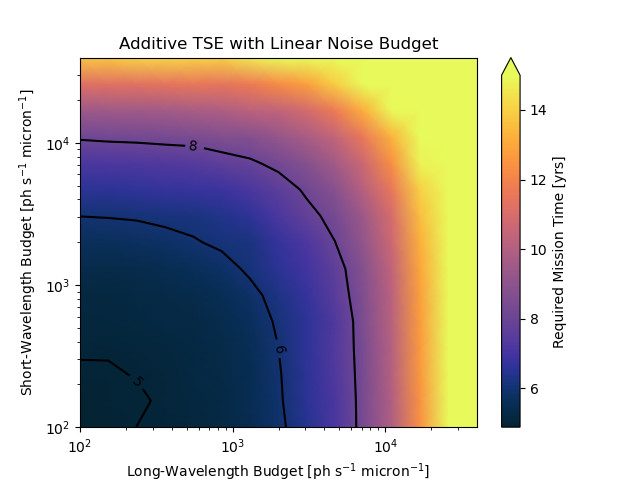
\includegraphics[width=\linewidth]{images/tse/tse_linear_additive_hab2hi.png}
%DIFDELCMD <         %%%
\DIFdelendFL \DIFaddbeginFL 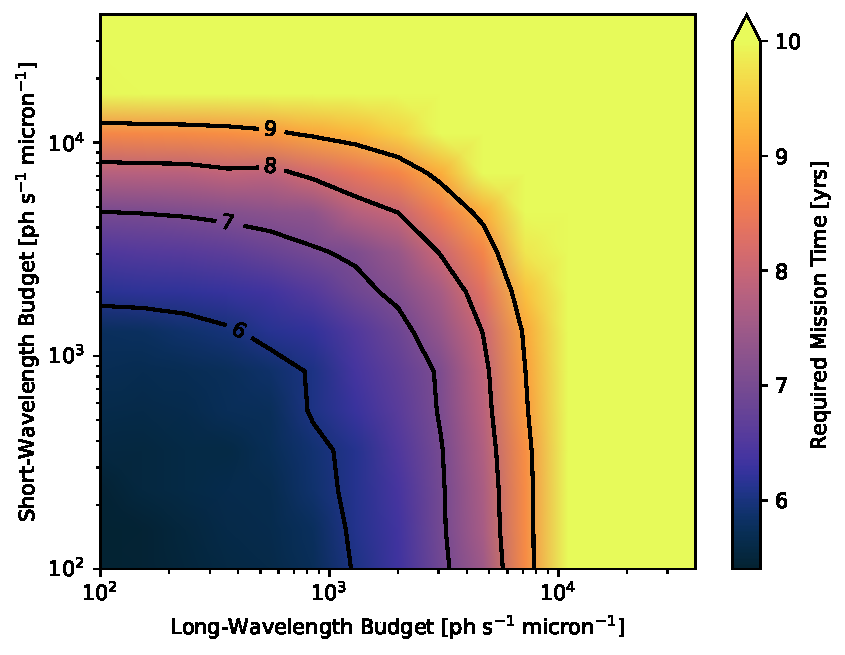
\includegraphics[width=\linewidth]{images/tse/final/no2_hi_linear.pdf}
        \DIFaddendFL \caption{\DIFaddbeginFL \DIFaddFL{Order 2, }\DIFaddendFL Hab2Max}
    \DIFdelbeginFL %DIFDELCMD < \label{fig: tse linear additive a}
%DIFDELCMD <     %%%
\DIFdelendFL \end{subfigure}
    \begin{subfigure}{.49\textwidth}
        \centering
        \DIFdelbeginFL %DIFDELCMD < 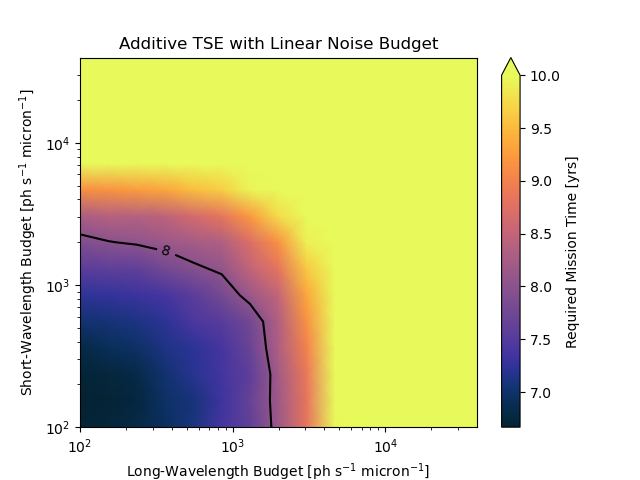
\includegraphics[width=\linewidth]{images/tse/tse_linear_additive_hab2lo.png}
%DIFDELCMD <         %%%
\DIFdelendFL \DIFaddbeginFL 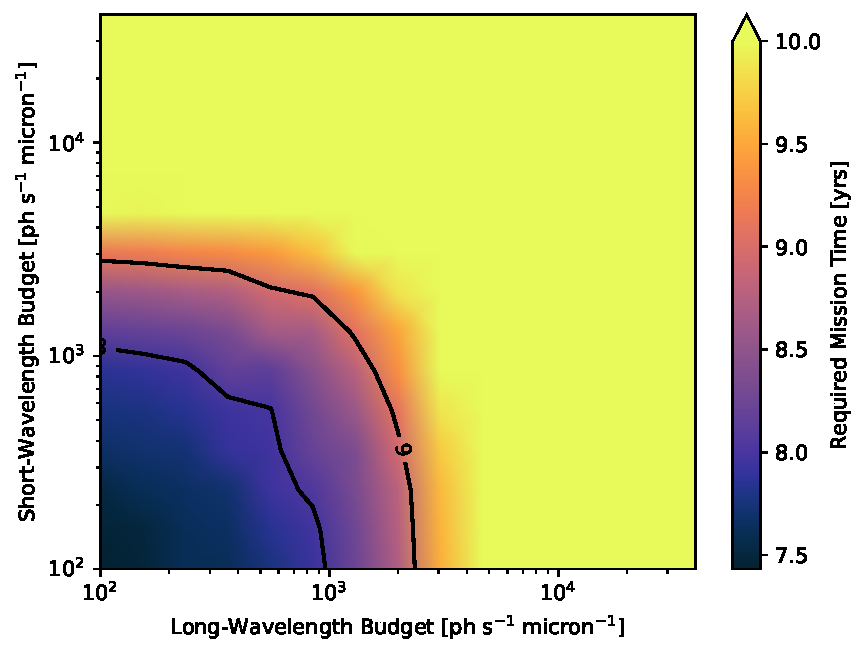
\includegraphics[width=\linewidth]{images/tse/final/no2_lo_linear.pdf}
        \DIFaddendFL \caption{\DIFaddbeginFL \DIFaddFL{Order 2, }\DIFaddendFL Hab2Min}
    \DIFdelbeginFL %DIFDELCMD < \label{fig: tse linear additive b}
%DIFDELCMD <     %%%
\DIFdelendFL \end{subfigure}
    \DIFaddbeginFL \begin{subfigure}{.49\textwidth}
        \centering
        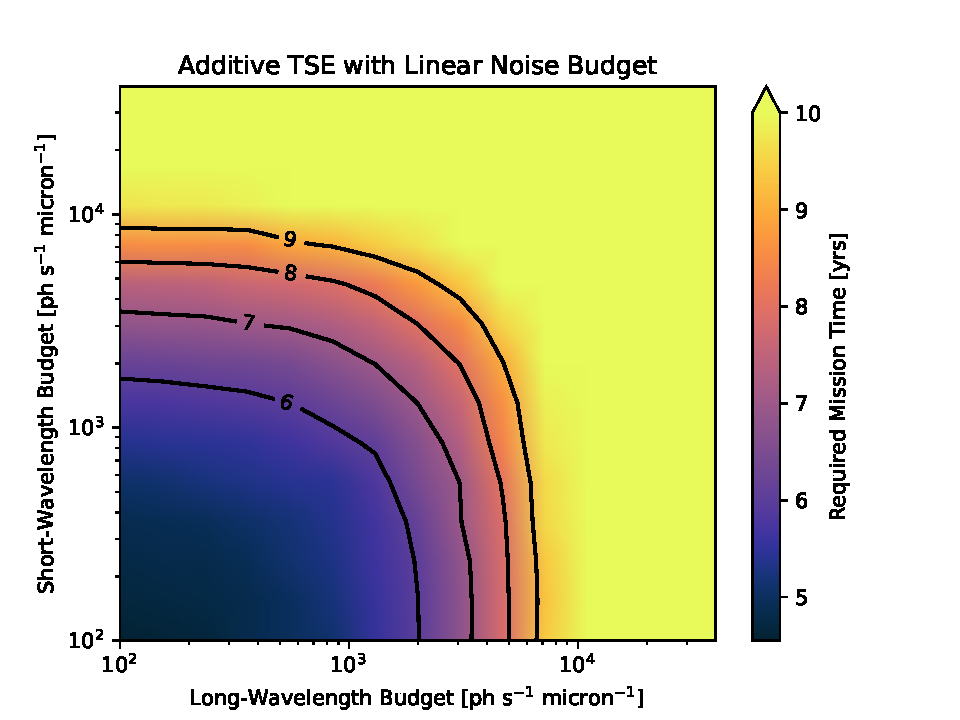
\includegraphics[width=\linewidth]{images/tse/final/no4_hi_linear.pdf}
        \DIFaddendFL \caption{\DIFdelbeginFL \DIFdelFL{Required mission time over a grid of short- and long-wavelength endpoints of a linear additive noise budget}\DIFdelendFL \DIFaddbeginFL \DIFaddFL{Order 4}\DIFaddendFL , \DIFdelbeginFL \DIFdelFL{at a limiting magnitude of 7, a field of regard of $65^\circ$ and a slew time of 12\,h, for a null order of two. Black contours mark integer mission-time levels. In both catalogs the contours extend further along the short-wavelength axis than the long-wavelength axis, showing that noise added at long wavelengths costs more mission time. The Hab2Min catalog (b) reaches its mission-time cap at much lower budgets, reflecting its lower planet occurrence.}\DIFdelendFL \DIFaddbeginFL \DIFaddFL{Hab2Max}\DIFaddendFL }
    \DIFaddbeginFL \end{subfigure}
    \begin{subfigure}{.49\textwidth}
        \centering
        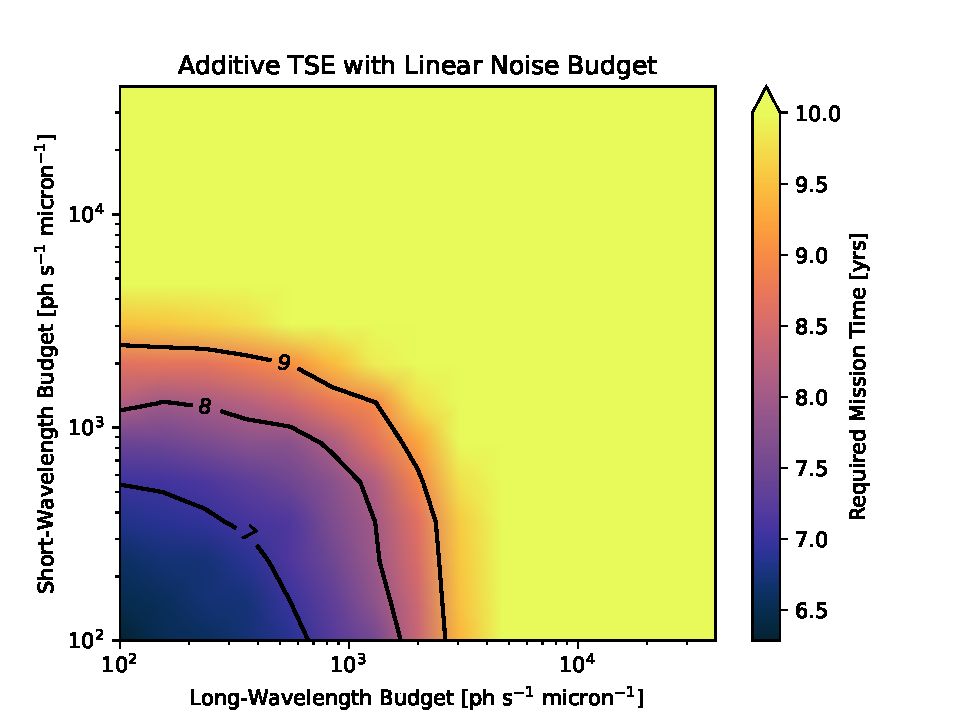
\includegraphics[width=\linewidth]{images/tse/final/no4_lo_linear.pdf}
        \caption{\DIFaddFL{Order 4, Hab2Min}}
    \end{subfigure}
    \caption{\DIFaddFL{Required mission time over independent short- and long-wavelength ramp endpoints at magnitude 7, FoR $65^\circ$, and slew 12\,h. Black curves mark integer mission-time contours. The preferred axis reverses between null orders in both catalogs.}}
    \DIFaddendFL \label{fig: tse linear additive}
\end{figure}

\subsection{The Random-Noise Error Budget} \label{sec: tse: budget result}
\DIFdelbegin \DIFdel{We can now state the central result of this thesis. Combining the two findings above, the affordable budget is largest when it is shaped to follow the stellar leakage, i.e. concentrated toward the short wavelengths. Taking this most permissive shape, Table \ref{tab: budget result} gives the resulting random-noise error budget as a spectral density at representative wavelengths, for the optimistic Hab2Max catalog at a five-year target and the pessimistic Hab2Min catalog at a seven-year target, both at a null order of two and the operating point of Fig. \ref{fig: tse budget shapes}. The Hab2Min budget is read from its seven-year run, shown in Fig. \ref{fig: tse budget hab2min}. In both cases the budget is a linear ramp, peaking at the short-wavelength end and falling to zero near 17\,$\upmu$m, so that essentially no additional noise is permissible in the zodiacal-dominated long-wavelength region}\DIFdelend \DIFaddbegin \DIFadd{Table \ref{tab: budget shapes} is the numerical answer to the central research question for the tested families and operating points. For any chosen row and shape, amplitudes below the reported value satisfy the corresponding mission-time target under the monotonic-search assumption. The flat family is the most directly comparable scalar allowance. The ramps test where added random variance is least damaging, but their unequal spectral integrals mean that their endpoint amplitudes must not be interpreted as a global cost ranking}\DIFaddend .

\DIFdelbegin %DIFDELCMD < \begin{table}[htbp]
%DIFDELCMD < \centering
%DIFDELCMD < \begin{tabular}{@{}ccc@{}}
%DIFDELCMD < \toprule
%DIFDELCMD < %%%
\DIFdelFL{Wavelength }%DIFDELCMD < & %%%
%DIFDELCMD < \multicolumn{2}{c}{%
{%DIFAUXCMD
\DIFdelFL{Allowable random-noise budget }%DIFDELCMD < [%%%
\DIFdelFL{ph\,s$^{-1}$}%DIFDELCMD < {}%%%
\DIFdelFL{$\upmu$m$^{-1}$}%DIFDELCMD < ]%%%
} %DIFAUXCMD
%DIFDELCMD < \\
%DIFDELCMD < \cmidrule%%%
\DIFdelFL{(l)}%DIFDELCMD < {%%%
\DIFdelFL{2-3}%DIFDELCMD < }
%DIFDELCMD < %%%
\DIFdelFL{$[\upmu\mathrm{m}]$ }%DIFDELCMD < & %%%
\DIFdelFL{Hab2Max (5 yr) }%DIFDELCMD < & %%%
\DIFdelFL{Hab2Min (7 yr) }%DIFDELCMD < \\
%DIFDELCMD < \midrule
%DIFDELCMD < %%%
\DIFdelFL{4  }%DIFDELCMD < & %%%
\DIFdelFL{470 }%DIFDELCMD < & %%%
\DIFdelFL{730 }%DIFDELCMD < \\
%DIFDELCMD < %%%
\DIFdelFL{6  }%DIFDELCMD < & %%%
\DIFdelFL{400 }%DIFDELCMD < & %%%
\DIFdelFL{620 }%DIFDELCMD < \\
%DIFDELCMD < %%%
\DIFdelFL{8  }%DIFDELCMD < & %%%
\DIFdelFL{320 }%DIFDELCMD < & %%%
\DIFdelFL{505 }%DIFDELCMD < \\
%DIFDELCMD < %%%
\DIFdelFL{10 }%DIFDELCMD < & %%%
\DIFdelFL{250 }%DIFDELCMD < & %%%
\DIFdelFL{395 }%DIFDELCMD < \\
%DIFDELCMD < %%%
\DIFdelFL{12 }%DIFDELCMD < & %%%
\DIFdelFL{180 }%DIFDELCMD < & %%%
\DIFdelFL{280 }%DIFDELCMD < \\
%DIFDELCMD < %%%
\DIFdelFL{14 }%DIFDELCMD < & %%%
\DIFdelFL{110 }%DIFDELCMD < & %%%
\DIFdelFL{170 }%DIFDELCMD < \\
%DIFDELCMD < %%%
\DIFdelFL{16 }%DIFDELCMD < & %%%
\DIFdelFL{40  }%DIFDELCMD < & %%%
\DIFdelFL{55  }%DIFDELCMD < \\
%DIFDELCMD < \bottomrule
%DIFDELCMD < \end{tabular}
%DIFDELCMD < %%%
%DIFDELCMD < \caption{%
{%DIFAUXCMD
\DIFdelFL{The central result: the instrument-agnostic random-noise error budget as a function of wavelength, for the short-weighted (leakage-shaped) distribution that maximizes the affordable budget. An instrument whose random-noise spectral density stays below these values at every wavelength completes Experiment 1 within the stated mission time. Both columns are the linear budget ramp evaluated at each wavelength, with short-wavelength endpoints of 470 ph\,s$^{-1}$}%DIFDELCMD < {}%%%
\DIFdelFL{$\upmu$m$^{-1}$ for Hab2Max and 730 for Hab2Min, falling linearly to zero toward 17\,$\upmu$m (Fig. \ref{fig: tse budget shapes} and Fig. \ref{fig: tse budget hab2min}).}}
%DIFAUXCMD
%DIFDELCMD < \label{tab: budget result}
%DIFDELCMD < \end{table}
%DIFDELCMD < 

%DIFDELCMD < \begin{figure}[htbp]
%DIFDELCMD <     \centering
%DIFDELCMD <     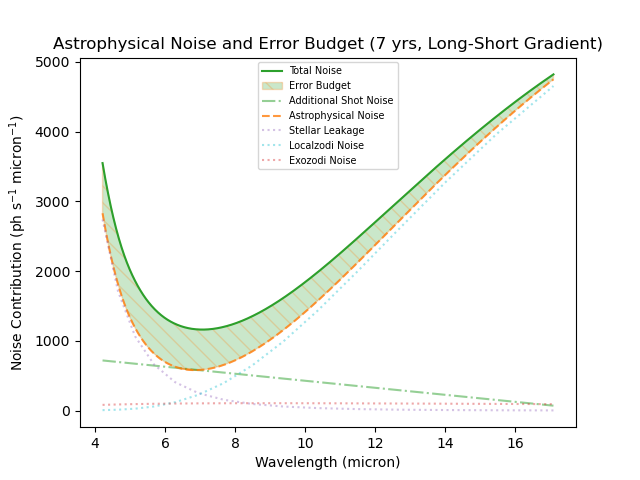
\includegraphics[width=0.6\linewidth]{images/tse/tse_budget_shortlong_hab2min_7yr.png}
%DIFDELCMD <     %%%
%DIFDELCMD < \caption{%
{%DIFAUXCMD
\DIFdelFL{The short-weighted (leakage-shaped) error budget for the Hab2Min catalog at a seven-year target, from which the Hab2Min column of Table \ref{tab: budget result} is read. Curves as in Fig. \ref{fig: tse budget shapes}; the added budget (green dash-dot) peaks at 730 ph\,s$^{-1}$}%DIFDELCMD < {}%%%
\DIFdelFL{$\upmu$m$^{-1}$ at the short-wavelength end and ramps linearly to zero near 17\,$\upmu$m.}}
    %DIFAUXCMD
%DIFDELCMD < \label{fig: tse budget hab2min}
%DIFDELCMD < \end{figure}
%DIFDELCMD < 

%DIFDELCMD < %%%
\DIFdel{This table is the concrete, instrument-agnostic answer to the central research question of Section \ref{sec: intro: research questions}: for the double Bracewell architecture it states, wavelength by wavelength, how much random instrumental noise the LIFE instrument may carry while still characterizing the required sample of terrestrial planets within a five- to seven-year mission, depending on the assumed planet occurrence rate. Because the budget is derived from the astrophysical limit upward and expressed independently of any specific noise mechanism, it applies to whatever combination of instrumental effects an eventual design produces, as long as their summed random-noise spectral density respects these bounds}\DIFdelend \DIFaddbegin \DIFadd{The result also does not provide independent limits at individual wavelengths. For example, the zero at one end of a ramp is imposed by its definition, not inferred from the experiment. Converting these aggregate allowances into an instrument requirement requires a separate allocation model that maps subsystem noise terms to the same reference plane and combines their independent variances}\DIFaddend .

\subsection{Dependence on the Agnostic Parameters}
The \DIFdelbegin \DIFdel{affordable budget is not a single number but a function of the agnostic operating point defined in Section \ref{sec: intro: params}. We map it over the two most consequential pairs of agnostic parameters , holding the budget flat in wavelength}\DIFdelend \DIFaddbegin \DIFadd{remaining scans use the flat budget and vary two agnostic parameters at a time. They therefore show operating-point dependence of the flat allowance and cannot automatically be transferred to either ramp family}\DIFaddend .

\DIFdelbegin \DIFdel{Fig. }\DIFdelend \DIFaddbegin \DIFadd{Figure }\DIFaddend \ref{fig: tse iso magfor} \DIFdelbegin \DIFdel{scans the limiting magnitude against the }\DIFdelend \DIFaddbegin \DIFadd{varies limiting magnitude and }\DIFaddend field of regard \DIFdelbegin \DIFdel{. The dominant lever is unambiguously }\DIFdelend \DIFaddbegin \DIFadd{at fixed 12\,h slew time. In all four panels, widening }\DIFaddend the field of regard \DIFdelbegin \DIFdel{. Below roughly $58^\circ$ the five-year target for Hab2Max is unreachable at any magnitude, even with zero added noise: the field-of-regard cut removes too many targets. Above that threshold the affordable budget rises steeply with widening field of regard, crossing 500 ph\,s$^{-1}$}%DIFDELCMD < {}%%%
\DIFdel{$\upmu$m$^{-1}$ near $76^\circ$ and reaching about 850 at the full $90^\circ$. The dependence on limiting magnitude is by comparison weak and saturating }\DIFdelend \DIFaddbegin \DIFadd{has the larger effect because it admits more potential targets. The magnitude dependence largely saturates near the adopted value of 7, especially }\DIFaddend for Hab2Max: once \DIFdelbegin \DIFdel{the magnitude is faint enough to include the targets that actually constrain the mission, going fainter adds little. The reason the field of regard is so decisive is geometric, and is made explicit in Fig. \ref{fig: tse yield}: the cut excises two polar wedges, a "zone of avoidance", from the sky, and at a $65^\circ$ field of regard this already removes $26.7\%$ of the otherwise interesting targets}\DIFdelend \DIFaddbegin \DIFadd{most high-SNR qualifying stars pass the magnitude cut, admitting still fainter targets adds little to the optimized top-50 sample. Field of regard acts differently because it removes entire sky regions irrespective of target brightness. The fourth-order proxy generally permits a larger flat allowance, but the same qualitative filter dependence remains}\DIFaddend .

\begin{figure}[htbp]
    \centering
    \begin{subfigure}{.49\textwidth}
        \centering
        \DIFdelbeginFL %DIFDELCMD < 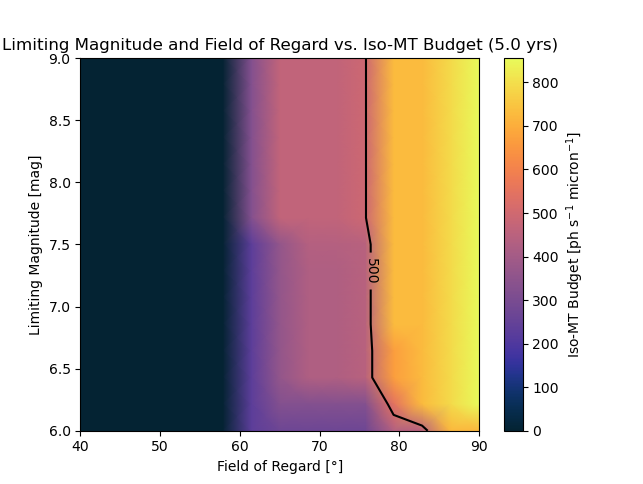
\includegraphics[width=\linewidth]{images/tse/tse_iso_magfor_hab2hi_5yr.png}
%DIFDELCMD <         %%%
\DIFdelendFL \DIFaddbeginFL 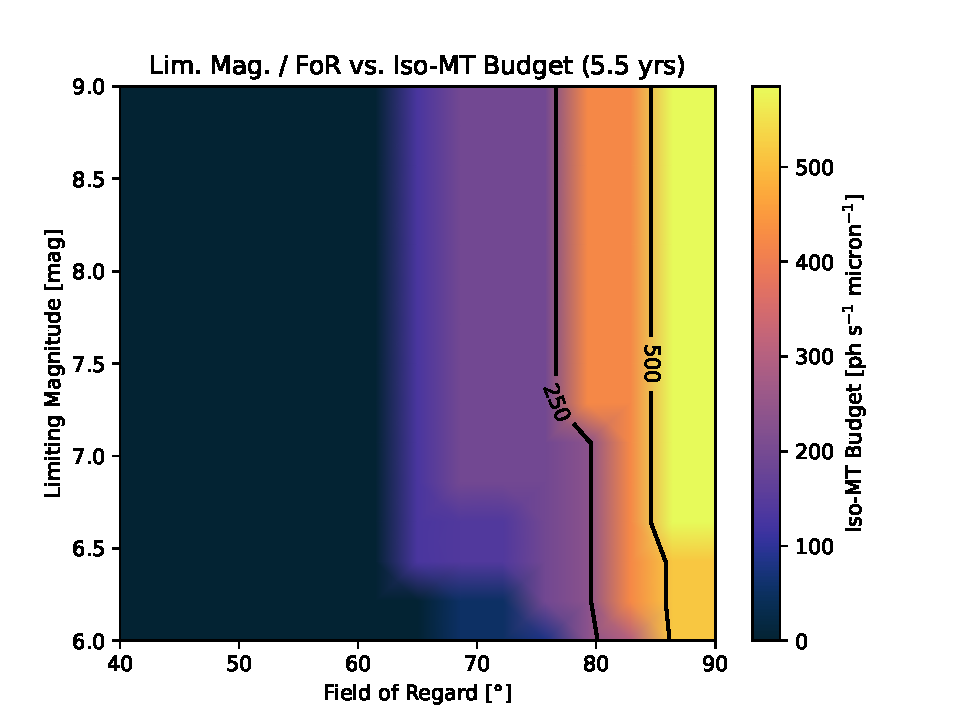
\includegraphics[width=\linewidth]{images/tse/final/no2_hi_magfor_5p5.pdf}
        \DIFaddendFL \caption{\DIFaddbeginFL \DIFaddFL{Order 2, }\DIFaddendFL Hab2Max, \DIFdelbeginFL \DIFdelFL{5-year target}\DIFdelendFL \DIFaddbeginFL \DIFaddFL{5.5\,yr}\DIFaddendFL }
    \DIFdelbeginFL %DIFDELCMD < \label{fig: tse iso magfor a}
%DIFDELCMD <     %%%
\DIFdelendFL \end{subfigure}
    \begin{subfigure}{.49\textwidth}
        \centering
        \DIFdelbeginFL %DIFDELCMD < 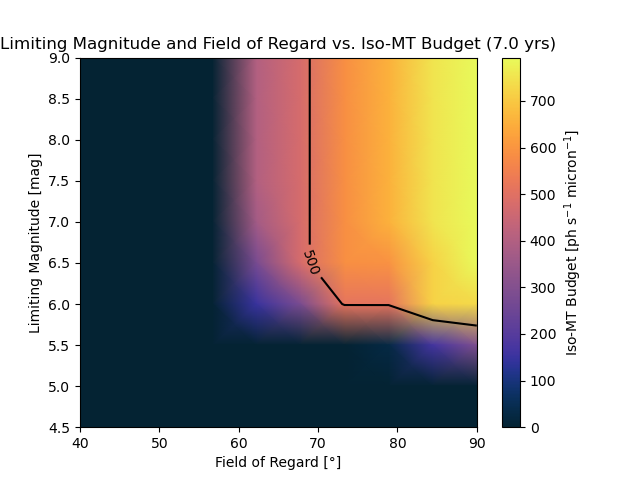
\includegraphics[width=\linewidth]{images/tse/tse_iso_magfor_hab2lo_7yr.png}
%DIFDELCMD <         %%%
\DIFdelendFL \DIFaddbeginFL 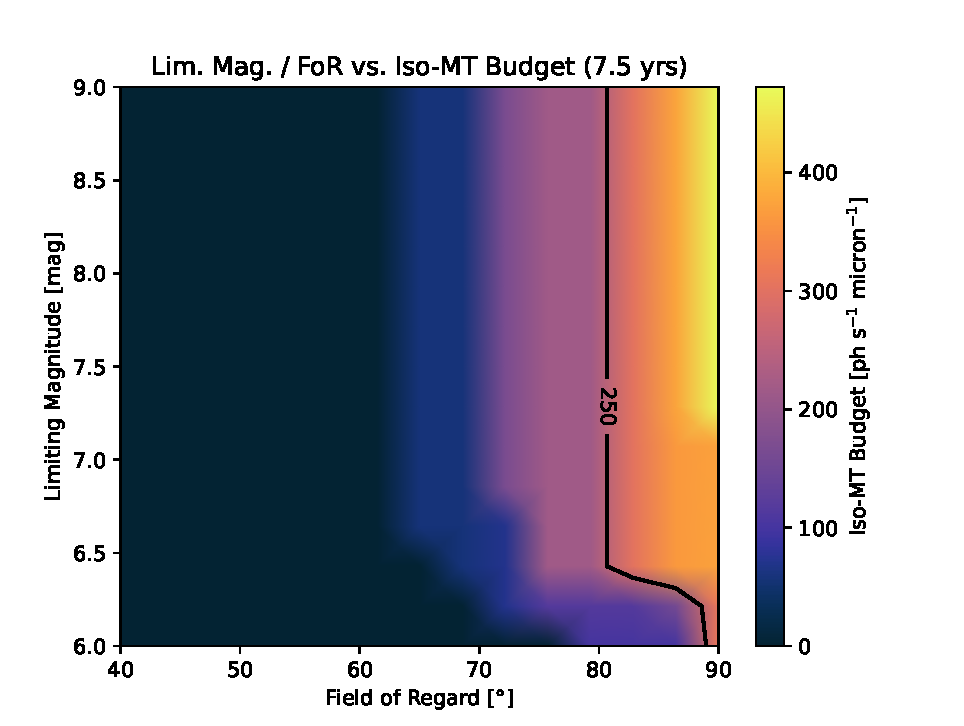
\includegraphics[width=\linewidth]{images/tse/final/no2_lo_magfor_7p5.pdf}
        \DIFaddendFL \caption{\DIFaddbeginFL \DIFaddFL{Order 2, }\DIFaddendFL Hab2Min, \DIFdelbeginFL \DIFdelFL{7-year target}\DIFdelendFL \DIFaddbeginFL \DIFaddFL{7.5\,yr}\DIFaddendFL }
    \DIFdelbeginFL %DIFDELCMD < \label{fig: tse iso magfor b}
%DIFDELCMD <     %%%
\DIFdelendFL \end{subfigure}
    \DIFaddbeginFL \begin{subfigure}{.49\textwidth}
        \centering
        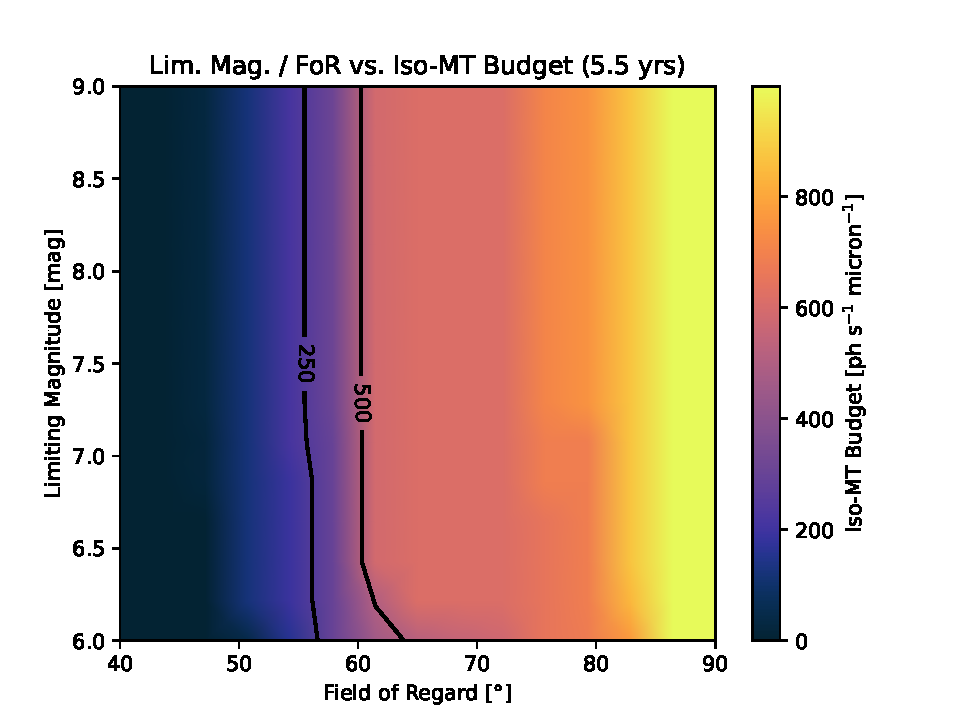
\includegraphics[width=\linewidth]{images/tse/final/no4_hi_magfor_5p5.pdf}
        \DIFaddendFL \caption{\DIFdelbeginFL \DIFdelFL{Iso-mission-time flat additive budget over limiting magnitude and field of regard}\DIFdelendFL \DIFaddbeginFL \DIFaddFL{Order 4}\DIFaddendFL , \DIFdelbeginFL \DIFdelFL{for a null order of two and a fixed slew time. Dark regions are infeasible (no budget permissible even without added noise). The field of regard is the dominant parameter in both catalogs; the dependence on limiting magnitude saturates for }\DIFdelendFL Hab2Max\DIFdelbeginFL \DIFdelFL{(a) but continues to help toward fainter magnitudes for the sparser Hab2Min (b). }\textbf{\DIFdelFL{TODO: ST mismatch: these are run at ST 10h, whereas the other plots use 12\,h!!}}%DIFAUXCMD
\DIFdelendFL \DIFaddbeginFL \DIFaddFL{, 5.5\,yr}\DIFaddendFL }
    \DIFaddbeginFL \end{subfigure}
    \begin{subfigure}{.49\textwidth}
        \centering
        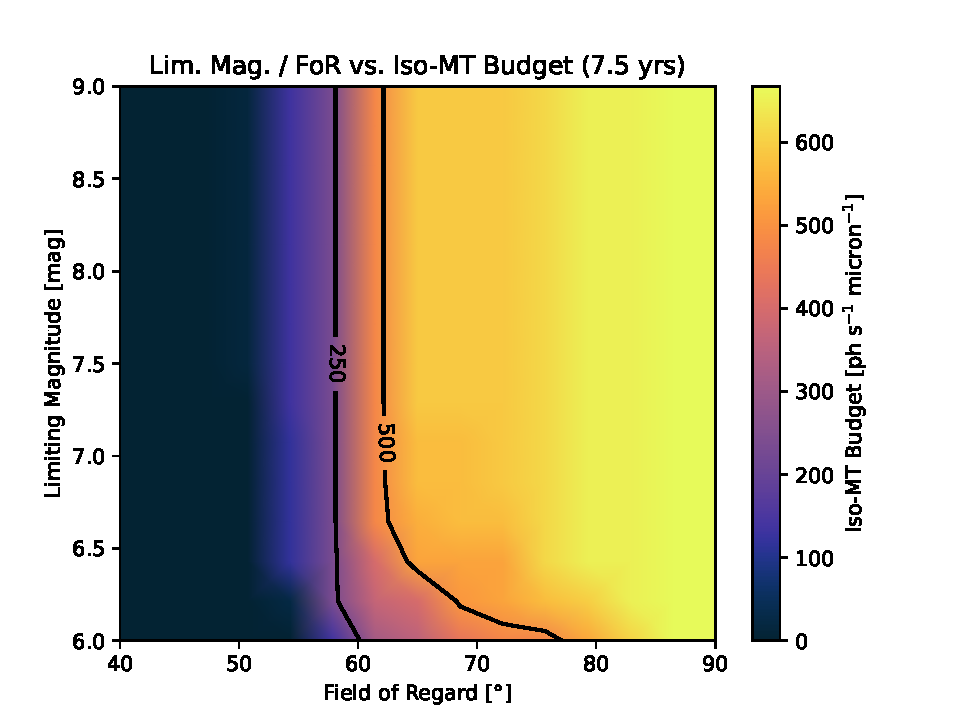
\includegraphics[width=\linewidth]{images/tse/final/no4_lo_magfor_7p5.pdf}
        \caption{\DIFaddFL{Order 4, Hab2Min, 7.5\,yr}}
    \end{subfigure}
    \caption{\DIFaddFL{Final iso-mission-time flat-budget scans over limiting magnitude and field of regard, with slew time fixed at 12\,h. Dark regions have no admissible positive budget at the corresponding operating point.}}
    \DIFaddendFL \label{fig: tse iso magfor}
\end{figure}

\DIFdelbegin \DIFdel{Fig. }\DIFdelend \DIFaddbegin \DIFadd{Figure }\DIFaddend \ref{fig: tse iso slewfor} \DIFdelbegin \DIFdel{scans the slew time against the }\DIFdelend \DIFaddbegin \DIFadd{varies slew time and }\DIFaddend field of regard at \DIFdelbegin \DIFdel{a }\DIFdelend fixed limiting magnitude \DIFdelbegin \DIFdel{of }\DIFdelend 7. \DIFdelbegin \DIFdel{Slew time enters the mission time directly as a per-retargeting overhead (Section \ref{sec: methods: AMS}), and the map shows how sharply it caps the budget: the affordable budget is largest at the bottom-right corner of short slew and wide field of regard, exceeding 2000 ph\,s$^{-1}$}%DIFDELCMD < {}%%%
\DIFdel{$\upmu$m$^{-1}$ for Hab2Max at a one-hour slew and $90^\circ$, and falls below 500 once the slew time exceeds roughly 13\,h even at the widest field of regard. Fast retargeting and a wide }\DIFdelend \DIFaddbegin \DIFadd{Longer slews consume time without adding SNR and therefore reduce the admissible budget. The dependence is especially important because each selected planet receives multiple follow-up visits: slew overhead is charged during the shared detection campaign, four additional orbit epochs, and characterization. Wide }\DIFaddend field of regard \DIFdelbegin \DIFdel{are thus the two operating conditions that most enlarge the permissible noise budget}\DIFdelend \DIFaddbegin \DIFadd{and short slew time therefore act together: more targets are available and less overhead is charged for moving between them}\DIFaddend .

\begin{figure}[htbp]
    \centering
    \begin{subfigure}{.49\textwidth}
        \centering
        \DIFdelbeginFL %DIFDELCMD < 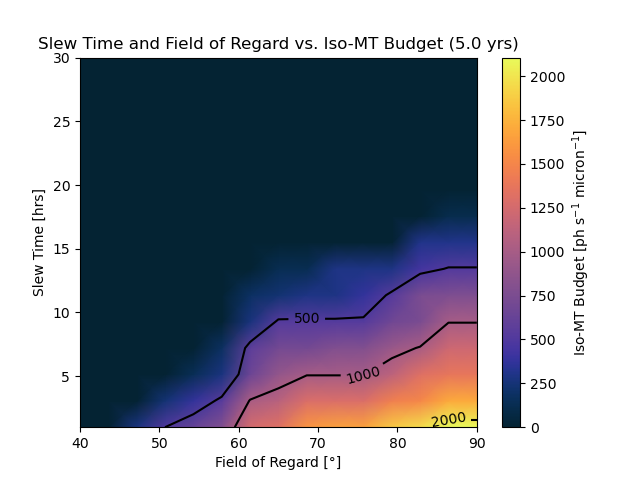
\includegraphics[width=\linewidth]{images/tse/tse_iso_slewfor_hab2hi_5yr.png}
%DIFDELCMD <         %%%
\DIFdelendFL \DIFaddbeginFL 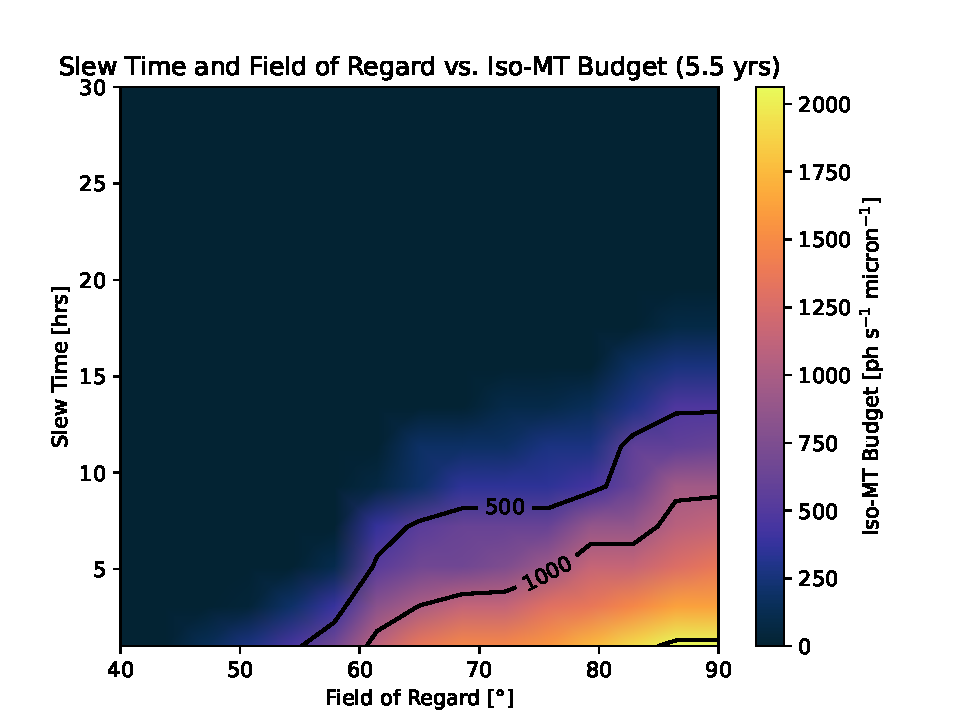
\includegraphics[width=\linewidth]{images/tse/final/no2_hi_slewfor_5p5.pdf}
        \DIFaddendFL \caption{\DIFaddbeginFL \DIFaddFL{Order 2, }\DIFaddendFL Hab2Max, \DIFdelbeginFL \DIFdelFL{5-year target}\DIFdelendFL \DIFaddbeginFL \DIFaddFL{5.5\,yr}\DIFaddendFL }
    \DIFdelbeginFL %DIFDELCMD < \label{fig: tse iso slewfor a}
%DIFDELCMD <     %%%
\DIFdelendFL \end{subfigure}
    \begin{subfigure}{.49\textwidth}
        \centering
        \DIFdelbeginFL %DIFDELCMD < 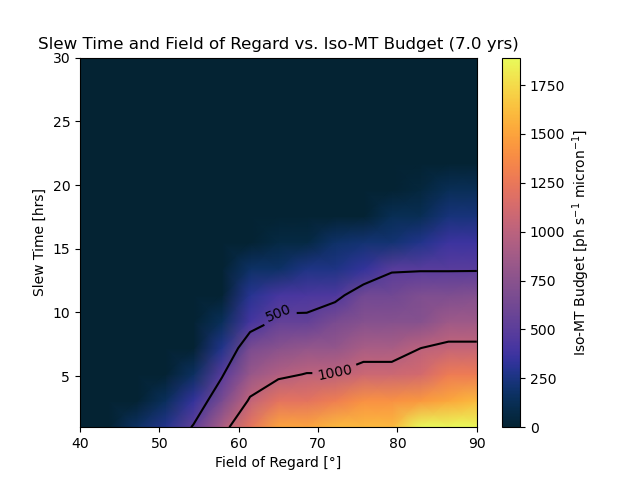
\includegraphics[width=\linewidth]{images/tse/tse_iso_slewfor_hab2lo_7yr.png}
%DIFDELCMD <         %%%
\DIFdelendFL \DIFaddbeginFL 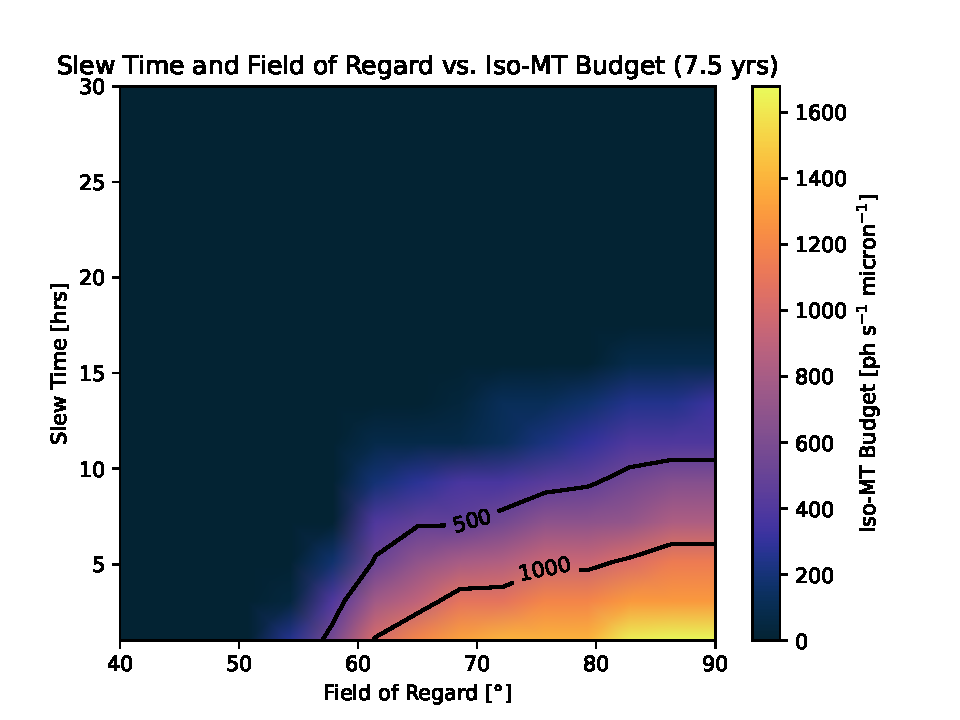
\includegraphics[width=\linewidth]{images/tse/final/no2_lo_slewfor_7p5.pdf}
        \DIFaddendFL \caption{\DIFaddbeginFL \DIFaddFL{Order 2, }\DIFaddendFL Hab2Min, \DIFdelbeginFL \DIFdelFL{7-year target}\DIFdelendFL \DIFaddbeginFL \DIFaddFL{7.5\,yr}\DIFaddendFL }
    \DIFdelbeginFL %DIFDELCMD < \label{fig: tse iso slewfor b}
%DIFDELCMD <     %%%
\DIFdelendFL \end{subfigure}
    \DIFaddbeginFL \begin{subfigure}{.49\textwidth}
        \centering
        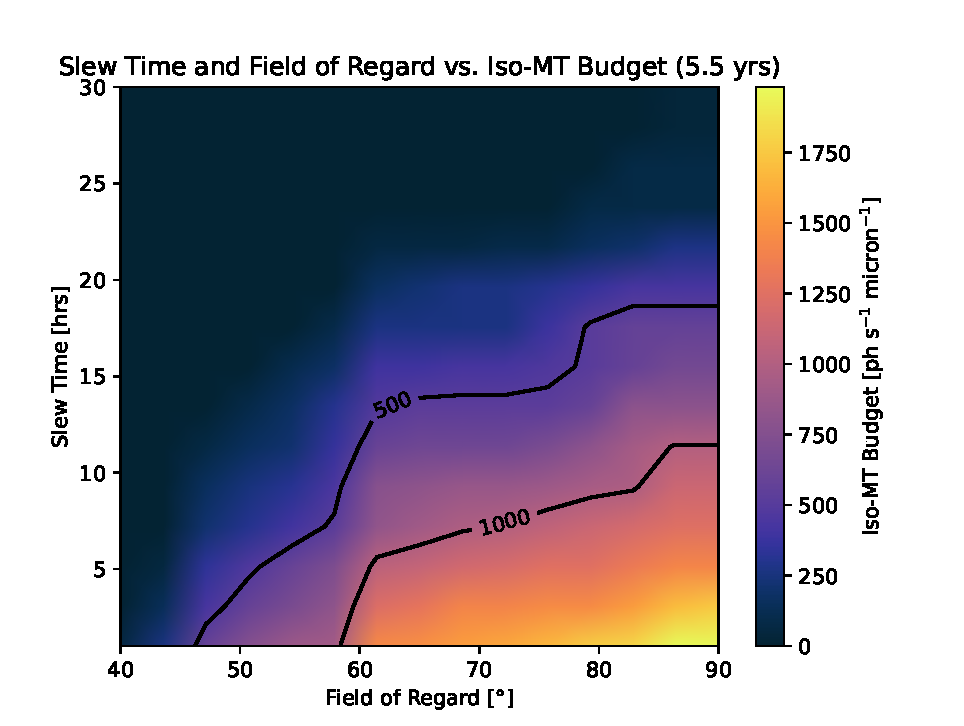
\includegraphics[width=\linewidth]{images/tse/final/no4_hi_slewfor_5p5.pdf}
        \DIFaddendFL \caption{\DIFdelbeginFL \DIFdelFL{Iso-mission-time flat additive budget over slew time and field of regard}\DIFdelendFL \DIFaddbeginFL \DIFaddFL{Order 4}\DIFaddendFL , \DIFdelbeginFL \DIFdelFL{for a null order of two and a fixed limiting magnitude of 7. The affordable budget falls steeply with increasing slew time}\DIFdelendFL \DIFaddbeginFL \DIFaddFL{Hab2Max}\DIFaddendFL , \DIFdelbeginFL \DIFdelFL{which is charged directly against the mission time, and grows with a widening field of regard. Both catalogs show the same structure, with Hab2Min (b) reaching lower budgets.}\DIFdelendFL \DIFaddbeginFL \DIFaddFL{5.5\,yr}\DIFaddendFL }
    \DIFaddbeginFL \end{subfigure}
    \begin{subfigure}{.49\textwidth}
        \centering
        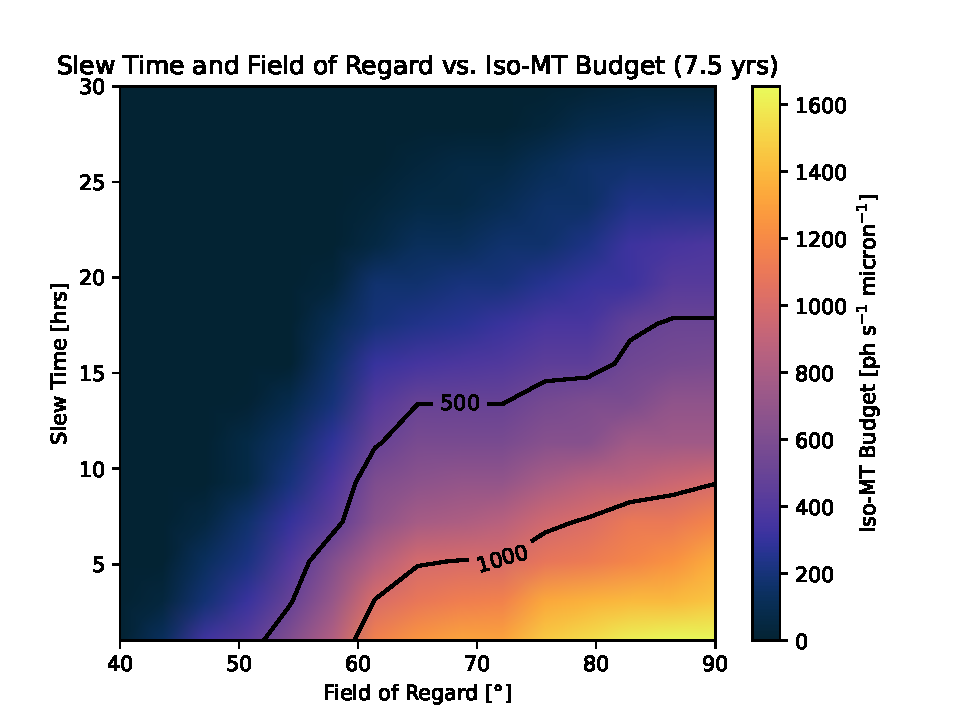
\includegraphics[width=\linewidth]{images/tse/final/no4_lo_slewfor_7p5.pdf}
        \caption{\DIFaddFL{Order 4, Hab2Min, 7.5\,yr}}
    \end{subfigure}
    \caption{\DIFaddFL{Final iso-mission-time flat-budget scans over slew time and field of regard at limiting magnitude 7. Dark regions have no admissible positive budget.}}
    \DIFaddendFL \label{fig: tse iso slewfor}
\end{figure}

\begin{figure}[htbp]
    \centering
    \DIFdelbeginFL %DIFDELCMD < 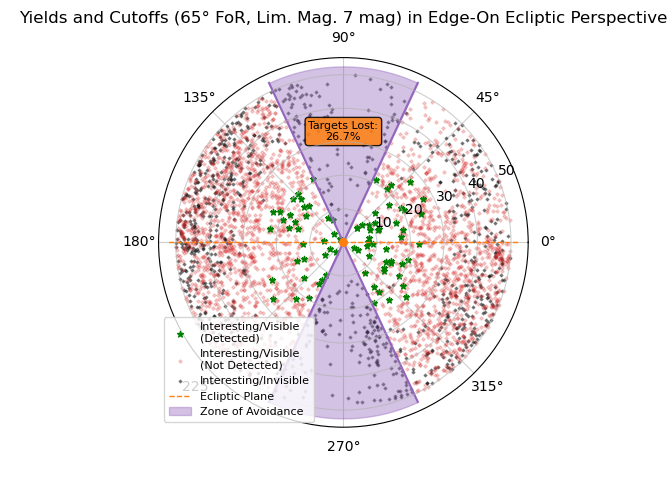
\includegraphics[width=0.7\linewidth]{images/tse/tse_yield_hab2hi.png}
%DIFDELCMD <     %%%
\DIFdelendFL \DIFaddbeginFL 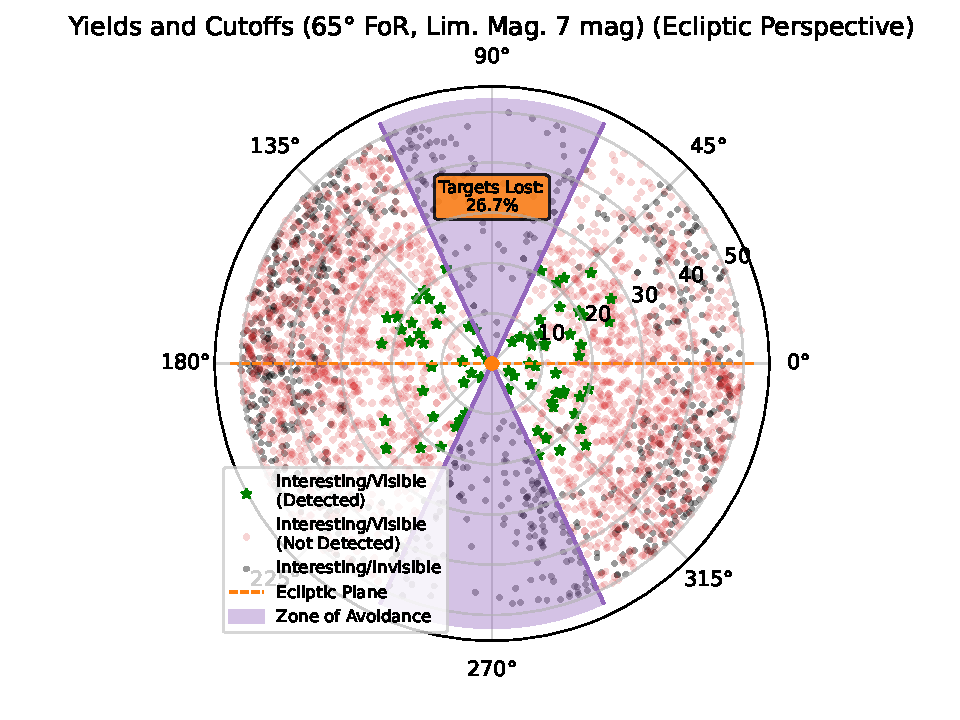
\includegraphics[width=0.7\linewidth]{images/tse/final/no2_hi_yield.pdf}
    \DIFaddendFL \caption{\DIFdelbeginFL \DIFdelFL{Edge-on ecliptic }\DIFdelendFL \DIFaddbeginFL \DIFaddFL{Ecliptic }\DIFaddendFL view of the \DIFdelbeginFL \DIFdelFL{target distribution for }\DIFdelendFL \DIFaddbeginFL \DIFaddFL{final }\DIFaddendFL Hab2Max \DIFaddbeginFL \DIFaddFL{selection }\DIFaddendFL at \DIFdelbeginFL \DIFdelFL{a limiting }\DIFdelendFL magnitude \DIFdelbeginFL \DIFdelFL{of }\DIFdelendFL 7 and \DIFdelbeginFL \DIFdelFL{a field of regard of }\DIFdelendFL \DIFaddbeginFL \DIFaddFL{FoR }\DIFaddendFL $65^\circ$. \DIFdelbeginFL \DIFdelFL{The radial coordinate is the distance to the star and the angular coordinate the ecliptic latitude. Green markers are }\DIFdelendFL \DIFaddbeginFL \DIFaddFL{Here ``}\DIFaddendFL interesting\DIFaddbeginFL \DIFaddFL{'' denotes Experiment-1-eligible }\DIFaddendFL targets\DIFdelbeginFL \DIFdelFL{that are detected, red are interesting but undetected, and black are interesting but rendered invisible by the cuts}\DIFdelendFL . The \DIFdelbeginFL \DIFdelFL{shaded polar wedges are the field-of-regard "zone of avoidance"; at $65^\circ$ it removes $26.7\%$ of the interesting targets. Detected targets concentrate near the ecliptic plane }\DIFdelendFL \DIFaddbeginFL \DIFaddFL{26.7\% value is specific to this catalog }\DIFaddendFL and \DIFdelbeginFL \DIFdelFL{at small distances}\DIFdelendFL \DIFaddbeginFL \DIFaddFL{selection}\DIFaddendFL .}
    \label{fig: tse yield}
\end{figure}

\subsection{Catalog Dependence}
\DIFdelbegin \DIFdel{Every scan was run for both the optimistic Hab2Max and the pessimistic Hab2Min catalog, which differ in their assumed Earth-twin occurrence rate $\eta_\oplus$ (Section \ref{sec: intro: catalog}). The two behave qualitatively identically, exhibiting the same short-versus-long budget asymmetry, the same dominance of the field of regard, }\DIFdelend \DIFaddbegin \DIFadd{The Hab2Min and Hab2Max calculations show the same qualitative shape ordering }\DIFaddend and the same \DIFdelbegin \DIFdel{steep budget growth with mission time. They differ quantitatively as expected: }\DIFdelend \DIFaddbegin \DIFadd{null-order inversion. }\DIFaddend Hab2Min \DIFdelbegin \DIFdel{, with fewer detectable planets, requires a longer mission for the same scientific yield and therefore affords a smaller budget at any fixed target time, or equivalently reaches a given budget only at a longer target time. This is why the Hab2Min figures are shown at seven- and ten-year targets where the }\DIFdelend \DIFaddbegin \DIFadd{requires longer mission-time targets and generally returns smaller allowances at otherwise matched operating parameters, consistent with its less favorable planet population. Because the adopted mission-time targets differ between catalogs, the numerical difference cannot be attributed to $\eta_\oplus$ alone. Figure \ref{fig: tse yield} illustrates the field-of-regard filter for one }\DIFaddend Hab2Max \DIFdelbegin \DIFdel{figures use five and six years.
The consistency of the qualitative structure across the two occurrence-rate assumptions is reassuring: the shape of the error budget, and the ranking of the agnostic parameters, does not depend on the still-uncertain value of $\eta_\oplus$. }\DIFdelend \DIFaddbegin \DIFadd{selection and is not evidence of catalog independence.
}\DIFaddend 

\DIFdelbegin \subsection{\DIFdel{Higher Null Orders}} %DIFAUXCMD
\addtocounter{subsection}{-1}%DIFAUXCMD
\DIFdelend \DIFaddbegin \subsection{\DIFadd{Why the Spectral Preference Reverses at Null Order Four}} \DIFaddend \label{sec: tse: null order}
\DIFdelbegin \textbf{\DIFdel{TODO: NO4 plots are dupes of NO2 -- regenerate the null-order-four runs, then analyse here.}} %DIFAUXCMD
\DIFdel{Once regenerated, this subsection will repeat the above exploration for a null order of four and compare the resulting error budgets to those of null order two, addressing the architecture-comparison part of the central research question (Section \ref{sec: intro: research questions}).
In particular, since a higher null order suppresses on-axis noise sources such as stellar leakage more strongly, we expect the short-wavelength part of the budget to be the most affected, but this remains to be verified.
}\DIFdelend \DIFaddbegin \DIFadd{Suppression of stellar leakage is the leading physical interpretation of the completed order-four comparison. Equation \ref{eq: leakage small star} predicts a fourth-to-second-order ratio of approximately $x^2/8$. Across the 4505 unique catalog stars, $x=2\pi bR_\star/\lambda$ remains above 0.005 over the modeled band, outside the cancellation-sensitive numerical regime of the direct Bessel sum. At 10\,$\upmu$m the median leakage ratio is about $6.3\times10^{-5}$; at 18.5\,$\upmu$m it is about $1.9\times10^{-5}$. Direct positive quadrature agrees with the analytic order-four response over the complete catalog range.
}\DIFaddend 

\DIFdelbegin \section{\DIFdel{Discussion}}
%DIFAUXCMD
\addtocounter{section}{-1}%DIFAUXCMD
\DIFdelend \DIFaddbegin \DIFadd{This suppression removes the high short-wave stellar-noise floor visible in Fig. \ref{fig: tse budget shapes no2}. Added short-wave variance then becomes comparatively expensive. The remaining local- and exo-zodiacal backgrounds dominate toward longer wavelengths, so a larger long-weighted endpoint can be hidden beneath their photon noise. This explanation is consistent with the reversal in Table \ref{tab: budget shapes} and Fig. \ref{fig: tse linear additive}; however, no ablation run isolates leakage suppression from the simultaneous extended-source and planet-throughput changes.
}\DIFaddend 

\DIFdelbegin \DIFdel{Very much TODO
}%DIFDELCMD < 

%DIFDELCMD < %%%
\DIFdel{This section discusses the parts of the project completed so far: the instrument-agnostic approach, the Agnostic Mission Simulator, the trade space reductions, }\DIFdelend \DIFaddbegin \DIFadd{The result is physical within the proxy but not a standalone architecture prediction. Without throughput normalization, the far-field average of the null envelope changes from $1/4$ at order two to $3/16$ at order four. Local-zodiacal transmission therefore falls by approximately 25\%, }\DIFaddend and the \DIFdelbegin \DIFdel{first exploration of the reduced trade space, which already yields a random-noise error budget for the double Bracewell architecture.
The one central result still outstanding, the comparison of nulling architectures, awaits the higher-null-order exploration and is deferred to the marked placeholder below. }\DIFdelend \DIFaddbegin \DIFadd{off-axis planet response also changes. The order-four result consequently combines deeper central suppression with a different throughput distribution while holding all other instrument parameters fixed.
}\DIFaddend 

\DIFdelbegin \DIFdel{Having laid out the instrument-agnostic approach, the Agnostic Mission Simulator, the trade space reductions, }\DIFdelend \DIFaddbegin \begin{table}[htbp]
\centering
\begin{tabular}{@{}p{0.28\linewidth}p{0.27\linewidth}p{0.34\linewidth}@{}}
\toprule
\DIFaddFL{Effect }& \DIFaddFL{Order-two reference }& \DIFaddFL{Order-four proxy consequence }\\
\midrule
\DIFaddFL{Near-axis stellar leakage }& \DIFaddFL{Leading term $x^2/32$ }& \DIFaddFL{Leading term $x^4/256$; median ratio $6.3\times10^{-5}$ at 10\,$\upmu$m }\\
\DIFaddFL{Extended-source envelope average }& \DIFaddFL{$1/4$ }& \DIFaddFL{$3/16$, a 25\% reduction before other weighting }\\
\DIFaddFL{Dominant short-wave background }& \DIFaddFL{Stellar leakage }& \DIFaddFL{Leakage largely removed; added short-wave variance becomes more costly }\\
\DIFaddFL{Least damaging tested ramp }& \DIFaddFL{Short-weighted }& \DIFaddFL{Long-weighted }\\
\DIFaddFL{Interpretation }& \DIFaddFL{Double-Bracewell reference }& \DIFaddFL{Controlled response proxy, not a realizable architecture }\\
\bottomrule
\end{tabular}
\caption{\DIFaddFL{Synthesis of the physical and numerical changes behind the null-order inversion.}}
\label{tab: null order synthesis}
\end{table}

\chapteropening{Discussion}{Interpreting the allowances, the null-order inversion, and their boundaries}
\DIFadd{The thesis asks two connected questions: how much aggregate random noise LIFE can tolerate at a chosen mission time, and how that allowance changes when the modeled central null becomes steeper. The completed results answer both within the controlled reference calculation before the methodological and architectural boundaries are considered.
}

\subsection{\DIFadd{The Error Budget and Architecture Comparison}}
\DIFadd{At the adopted operating point, the nominal second-order null permits flat allowances of 140\,ph\,s$^{-1}$\,$\upmu$m$^{-1}$ for Hab2Max at 5.5\,yr and 65 for Hab2Min at 7.5\,yr. Within the tested ramp families, short-weighted noise is least damaging because it is added where stellar leakage already dominates. This finding is specific to the second-order background hierarchy.
}

\DIFadd{The fourth-order proxy changes that hierarchy. Its corresponding flat allowances rise to 650 and 590, }\DIFaddend and the \DIFdelbegin \DIFdel{error budget they produce, we step back to assess what these pieces achieve and where their limits lie}\DIFdelend \DIFaddbegin \DIFadd{long-weighted ramp becomes least damaging. The inversion occurs in both catalogs and in the full two-endpoint contour scans. Its leading interpretation is geometric: the analytic $x^4$ term suppresses stellar leakage and removes much of the short-wave variance floor. The result is robust within the tested proxy, but the absolute improvement cannot be assigned solely to null depth because the proxy also changes extended-source and planet throughput}\DIFaddend .

\subsection{The Agnostic Approach and the AMS}
The \DIFdelbegin \DIFdel{central methodological contribution so far is the decoupling of }\DIFdelend \DIFaddbegin \DIFadd{methodological contribution is mechanism-agnostic treatment of an }\emph{\DIFadd{aggregate}} \DIFadd{independent random-noise allowance, rather than a subsystem allocation. This common reference-plane quantity allows science completion time to constrain a later engineering allocation without prematurely choosing the physical origin of every random term.
}

\DIFadd{The AMS separates its SNR and filter flows (Section \ref{sec: methods: AMS}). Magnitude, field-of-regard, and slew changes therefore reuse cached unfiltered SNRs, while physical or budget changes trigger recomputation. Host-star memoization further avoids repeated source calculations for planets sharing one star. These boundaries turn the repeated evaluations required by }\DIFaddend the \DIFdelbegin \DIFdel{error budget question from any fixed instrument.
By treating signal and noise as inputs constrained only by the astrophysical limit (Section \ref{sec: intro: varparams descr}), }\DIFdelend \DIFaddbegin \DIFadd{TSE from an impractical uniform grid into targeted inversions.
}

\subsection{\DIFadd{What the Reductions Buy}}
\DIFadd{The first reduction combines only independent random terms that can be referred to the same single-output plane as $N_I(\lambda)$ (Section \ref{sec: ts reduction: condensation}). The second replaces spatial-grid evaluation of symmetric backgrounds with exact azimuthal averages and one-dimensional radial quadrature. Together they reduce a formally infinite-dimensional problem to explicit scalar searches, remove image size as a production-science parameter, expose the local-zodiacal normalization error, }\DIFaddend and \DIFdelbegin \DIFdel{by approximating different nulling architectures through the modified null-depth ansatz (Section \ref{sec: intro: null depth approach}), we obtain a framework that never commits to a single interferometer layout. This is a genuine departure from the conventional workflow, in which a double Bracewell is assumed and the noise is derived from it.
The pay-off is that a single tool, the AMS, can in principle answer both open questions of the mission at once: how much random noise budget is affordable, and which null order spends that budget most economically. }\DIFdelend \DIFaddbegin \DIFadd{provide the analytic null-order scaling used to interpret the result.
}

\subsection{\DIFadd{Limitations}}
\DIFadd{Table \ref{tab: ranked limitations} ranks the remaining boundaries by their ability to change the numerical allowance or its engineering interpretation.
}

\begin{table}[htbp]
\centering
\small
\begin{tabular}{@{}p{0.09\linewidth}p{0.22\linewidth}p{0.60\linewidth}@{}}
\toprule
\DIFaddFL{Priority }& \DIFaddFL{Limitation }& \DIFaddFL{Consequence }\\
\midrule
\DIFaddFL{1 }& \DIFaddFL{Unnormalized null-order proxy }& \DIFaddFL{The order-four comparison combines deeper suppression with changed planet and extended-source throughput; it is not a design prediction. }\\
\DIFaddFL{2 }& \DIFaddFL{Scheduler boundary behavior }& \DIFaddFL{Strict completion tests require at least 51 detections in at least 91 universes, while empty universes are omitted. These choices can bias mission time in opposite directions. }\\
\DIFaddFL{3 }& \DIFaddFL{Aggregate random-noise model }& \DIFaddFL{Correlated instability, calibration bias, and systematic error cannot be allocated from $N_I$ and may impose stricter requirements. }\\
\DIFaddFL{4 }& \DIFaddFL{Sampling uncertainty }& \DIFaddFL{The 100 universes resolve only a sampled 90th percentile. Its 95.6\% distribution-free rank interval spans order statistics 84--96, but saved outputs do not retain the corresponding time amplitudes. }\\
\DIFaddFL{5 }& \DIFaddFL{Symmetric exozodiacal model }& \DIFaddFL{Inclined, clumpy, or asymmetric disks can create rotation-dependent structure absent from the face-on radial reduction. }\\
\DIFaddFL{6 }& \DIFaddFL{Tested spectral families }& \DIFaddFL{Flat and two linear ramps sample three directions in a functional trade space; endpoints are not independent wavelength limits or engineering-cost rankings. }\\
\bottomrule
\end{tabular}
\caption{\DIFaddFL{Ranked limitations of the reported error budgets. Priority reflects relevance to the thesis's central numerical and architectural claims, not ease of remediation.}}
\label{tab: ranked limitations}
\end{table}
\DIFaddend 

The \DIFdelbegin \DIFdel{AMS itself is built around one deliberate design decision, the separation of the SNR flow from the filter flow (Section \ref{sec: methods: AMS}). Because the physics-governing variable parameters change far less often than the agnostic cutoffs during an exploration, caching the unfiltered SNR array and re-running only the cheap filter step avoids a large amount of redundant computation. The stellar-physics memoization compounds this, since many planets share a host star. Together these make repeated AMS evaluations, the inner loop of any trade space exploration, affordable enough to contemplate at all. This matters directly: the naive grid estimate of Section \ref{sec: intro: trade space} put a brute-force scan at hundreds of years, so every constant factor saved in a single evaluation is what keeps the eventual exploration tractable}\DIFdelend \DIFaddbegin \DIFadd{first limitation sets the strongest boundary on the central comparison. Order four is an impact study of a steeper central null under retained assumptions, not a design prediction. It provides no realizable beam-combination matrix, aperture count, optical-loss model, instability-noise calculation, or control requirement. Likewise, the point estimates inherit both search tolerance and finite-universe rank uncertainty; neither is recoverable as a single symmetric error bar from the retained products}\DIFaddend .

\subsection{\DIFdelbegin \DIFdel{What the Reductions Buy}\DIFdelend \DIFaddbegin \DIFadd{Outlook}\DIFaddend }
The \DIFdelbegin \DIFdel{reductions of the previous chapter attack the trade spacefrom two independent directions. The condensation of astrophysical noise into a single additive, wavelength-dependent term $N_I(\lambda)$ (Section \ref{sec: ts reduction: condensation}) collapses what would otherwise be a separate budget per noise source into one interpretable function. This is not merely a computational convenience; it also keeps the final product, the error budget, in a form an instrument engineer can actually read and act on. We retain the wavelength dependence precisely because the blackbody character of the sources makes it physically indispensable, so the reduction trims dimensionality without discarding the one axis that carries physical meaning. }\DIFdelend \DIFaddbegin \DIFadd{next scientific step is not another run of the present trade space, but a more physical mapping. A realizable higher-order combiner should replace the $\sin^n$ proxy, including its aperture geometry, normalized throughput, optical losses, and instability terms. The aggregate allowance should then be allocated to concrete subsystems at the same reference plane.
}\DIFaddend 

\DIFdelbegin \DIFdel{The convergence study of the image size and spectral resolution (Section \ref{sec: ts reduction: image spec}) is a reduction of a different kind: it fixes two numerical knobs at the cheapest values that are still faithful.
The methodological lesson here is the one worth emphasizing.
    Convergence of a central value, a mean or a median, is not sufficient evidence that a setting is safe, because the average over a large catalog can look healthy while individual targets are badly wrong. Judging the spread alongside the mean is what exposes this, and it did so twice: the wide percentile band below 156 pixels, }\DIFdelend \DIFaddbegin \DIFadd{Before another production campaign, the scheduler should use non-strict completion criteria consistent with the stated experiment, retain failed universes explicitly, and save every per-universe component time. This would permit bootstrap or rank-based uncertainty intervals in years and separate detection, orbit, characterization, and slew sensitivities. Extending the analytic framework to inclined or asymmetric exozodiacal disks would remove the next important symmetry assumption. These steps would turn the present defensible impact study into a stronger architecture-level requirement analysis.
}

\chapteropening{Conclusion}{What the completed simulations establish---and what remains architecture-dependent}
\DIFadd{The completed AMS and TSE answer the central research question for every tested budget family and operating point. Under the approved physics model, the nominal second-order null permits primary flat allowances of 140\,ph\,s$^{-1}$\,$\upmu$m$^{-1}$ for Hab2Max at 5.5\,yr and 65 for Hab2Min at 7.5\,yr. The order-four proxy raises them to 650 }\DIFaddend and \DIFdelbegin \DIFdel{, more insidiously, the coincidental aliasing minimum at 100 pixels that dips in every statistic yet is a razor-thin, non-robust artifact rather than true convergence.
For a yield-driven mission , where a single grossly mis-sampled planet can distort the observation-time distribution, this per-target reliability is exactly the property that must be certified, not just the catalog average. Finally, the restriction of the null order to the physically realizable even values, and in practice to orders two and four (Section \ref{sec: intro: null depth approach}), reduces a continuous knob to a two-way comparison of clear engineering relevance. }\DIFdelend \DIFaddbegin \DIFadd{590, while the least damaging tested ramp reverses from short-weighted to long-weighted.
}

\DIFadd{The sub-questions close as follows:
}\begin{itemize}
    \item \DIFadd{The unrestricted AMS trade space contains up to eight free modifier functions and three scalar agnostic parameters and is therefore formally infinite-dimensional. The reported family searches reduce it to one amplitude dimension, four dimensions when all agnostic parameters vary, or five when two ramp endpoints vary independently.
    }\item \DIFadd{Magnitude, field-of-regard, and slew changes reuse unfiltered SNRs and repeat only filtering and scheduling. Budget, source-physics, or null-order changes require catalog-wide SNR recomputation, although host-shared source terms remain memoized within that pass.
    }\item \DIFadd{Combining independent random terms at one reference plane and analytically integrating symmetric backgrounds removes the unbounded functional and spatial-grid dimensions while reproducing the retained source calculation to the stated validation precision.
    }\item \DIFadd{The TSE locates maximum flat and linear-ramp amplitudes as iso-mission-time point estimates; Table \ref{tab: budget shapes} reports the complete set, including both catalogs and both mission-time targets.
    }\item \DIFadd{A fourth-order central null suppresses stellar leakage consistently with the analytic $x^4$ scaling and reverses the spectral preference in both catalogs. This is the leading physical interpretation within the proxy, not an isolated causal proof or a realizable architecture forecast.
}\end{itemize}
\DIFaddend 

\DIFdelbegin \subsection{\DIFdel{Limitations of the Current Groundwork}}
%DIFAUXCMD
\addtocounter{subsection}{-1}%DIFAUXCMD
\DIFdel{Several caveats bound the strength of the groundwork laid so far. }\DIFdelend \DIFaddbegin \DIFadd{These allowances do not yet constitute subsystem requirements. They define a validated bridge from scientific yield to an explicit engineering trade space and show which spectral regions most strongly control mission time. That bridge matters because LIFE's promise---new knowledge of nearby terrestrial planets and the possibility of life beyond Earth---depends not only on asking an ambitious question, but on demonstrating that an instrument can answer it within credible limits.
}

\appendix
\appendixchaptertrue

\chapteropening{Analytic Transmission Derivation}{Derivation of the circularly symmetric transmission and background response} \label{app: analytic derivation}
\DIFadd{This appendix records the reduction used by the production source model. It is included to make the fourth-order result independently inspectable without requiring the reader to reconstruct the mathematics from code.
}

\subsection{\DIFadd{Even-Power Reduction}}
\DIFadd{For a positive even null order $n=2p$, the nulling envelope can be written as a finite cosine series:
}\begin{align}
\DIFadd{\sin^{2p}x
=\frac{1}{4^p}\left[
\binom{2p}{p}
+2\sum_{j=1}^{p}(-1)^j
\binom{2p}{p-j}\cos(2jx)
\right].
\label{eq: sine power series}
}\end{align}
\DIFadd{One destructive output contains this envelope multiplied by an imaging factor $\cos^2(\psi\pm\pi/4)$. For an axisymmetric source, the complementary imaging phase contributes one half after full azimuthal integration. Let a sky point at angular radius $\vartheta$ have projected nulling coordinate $\alpha=\vartheta\cos\varphi$. Substituting $x=\pi b\vartheta\cos\varphi/\lambda$ into Eq. \ref{eq: sine power series} and using the NIST Digital Library of Mathematical Functions integral representation \mbox{%DIFAUXCMD
\cite{nistdlmf}}\hskip0pt%DIFAUXCMD
,
}\begin{align}
\DIFadd{\frac{1}{2\pi}\int_0^{2\pi}
\cos(z\cos\varphi)\,\mathrm{d}\varphi=J_0(z)
}\end{align}
\DIFadd{gives Eq. \ref{eq: general null average}. The reduction is exact for the proxy response and any circularly symmetric surface-brightness profile. It is not an approximation based on rapid rotation.
}

\DIFadd{For the two orders used in the thesis,
}\begin{align}
\DIFadd{\left\langle T_2\right\rangle_\varphi
}&\DIFadd{=\frac{1}{4}\left[1-J_0\left(\frac{2\pi b\vartheta}{\lambda}\right)\right],}\\
\DIFadd{\left\langle T_4\right\rangle_\varphi
}&\DIFadd{=\frac{1}{16}\left[
3-4J_0\left(\frac{2\pi b\vartheta}{\lambda}\right)
+J_0\left(\frac{4\pi b\vartheta}{\lambda}\right)
\right].
}\end{align}
\DIFadd{At large phase, the oscillatory Bessel terms approach zero. The corresponding far-field averages are therefore $1/4$ and $3/16$. This is the origin of the throughput caveat in the main text.
}

\subsection{\DIFadd{Uniform-Disk Average and Small-Star Limit}}
\DIFadd{For a uniform disk of angular radius $R$, area averaging a radial Bessel term gives, using the Bessel derivative identity \mbox{%DIFAUXCMD
\cite{nistdlmf}}\hskip0pt%DIFAUXCMD
,
}\begin{align}
\DIFadd{\frac{2}{R^2}\int_0^R
\vartheta J_0(a\vartheta)\,\mathrm{d}\vartheta
=\frac{2J_1(aR)}{aR}.
\label{eq: disk bessel average}
}\end{align}
\DIFaddend The \DIFdelbegin \DIFdel{modified null-depth ansatz reproduces the on-axis null order of a range of architectures but is explicitly a crude proxy: it inherits the double Bracewell baseline formalism and does not capture the full transmission geometry,
asymmetries, or aperture-count constraints of a real higher-order nuller. Its conclusions are therefore best read as a study of the }\textit{\DIFdel{impact}} %DIFAUXCMD
\DIFdel{of null order, not as a faithful simulation of any specific instrument. Likewise, condensing all instrumental noise into a single additive $N_I(\lambda)$ deliberately discards the distinction between noise origins; this is the right move for defining an overall budget, but it means the resulting budget speaks to the total allowable noise rather than to
any individual mechanism. The convergence conclusions, too, are stated for the background-limited regime the mission is designed for; were a strong per-channel detector floor to dominate, the spectral-resolution argument in particular would need revisiting, although we showed that such a floor only relaxes the image-size requirement. These are conscious trade-offs in the service of an interpretable, tractable budget, not oversights, but they delimit what the eventual numbers will and will not mean. }\DIFdelend \DIFaddbegin \DIFadd{right-hand side is evaluated as one when $aR=0$. With $x=2\pi bR/\lambda$, the disk-averaged responses become
}\begin{align}
\DIFadd{\left\langle T_2\right\rangle_\mathrm{disk}
}&\DIFadd{=\frac{1}{4}\left[1-\frac{2J_1(x)}{x}\right],}\\
\DIFadd{\left\langle T_4\right\rangle_\mathrm{disk}
}&\DIFadd{=\frac{1}{16}\left[
3-\frac{8J_1(x)}{x}+\frac{2J_1(2x)}{2x}
\right].
}\end{align}
\DIFadd{Using the standard Bessel power series \mbox{%DIFAUXCMD
\cite{nistdlmf}}\hskip0pt%DIFAUXCMD
, $J_1(x)=x/2-x^3/16+x^5/384+\mathcal{O}(x^7)$, which yields
}\begin{align}
\DIFadd{\left\langle T_2\right\rangle_\mathrm{disk}
}&\DIFadd{=\frac{x^2}{32}-\frac{x^4}{768}+\mathcal{O}(x^6),}\\
\DIFadd{\left\langle T_4\right\rangle_\mathrm{disk}
}&\DIFadd{=\frac{x^4}{256}+\mathcal{O}(x^6).
}\end{align}
\DIFadd{Consequently,
}\begin{align}
\DIFadd{\frac{\left\langle T_4\right\rangle_\mathrm{disk}}{\left\langle T_2\right\rangle_\mathrm{disk}}
=\frac{x^2}{8}+\mathcal{O}(x^4).
}\end{align}
\DIFadd{This scaling predicts the near-disappearance of geometric stellar leakage before any mission scheduling is performed. Direct positive quadrature is retained as a numerical safeguard where subtraction of nearly equal Bessel terms could lose precision.
}\DIFaddend 

\DIFdelbegin \subsection{\DIFdel{The Error Budget and Architecture Comparison}}
%DIFAUXCMD
\addtocounter{subsection}{-1}%DIFAUXCMD
\DIFdel{The trade space exploration of Section \ref{sec: tse} turns the machinery of this thesis into a concrete deliverable: a random-noise error budget for the LIFE instrument, tabulated as a function of wavelength in Table \ref{tab: budget result}. Its engineering-relevant features were established in Section \ref{sec: tse: budget result} and are only summarized here: the budget is strongly wavelength-dependent and most permissive when shaped like the stellar leakage, so that the zodiacal-dominated long wavelengths, which tolerate almost no added noise, are where the instrument must be built most cleanly;
    it grows close to exponentially with the permitted mission time;
    }\DIFdelend \DIFaddbegin \subsection{\DIFadd{Radial Profiles and Wavelength Bins}}
\DIFadd{For a circular source with surface brightness $I_\lambda(\vartheta)$, the transmitted spectral photon rate is proportional to
}\begin{align}
\DIFadd{2\pi\int_0^{R_\mathrm{max}}
I_\lambda(\vartheta)
\left\langle T_n\right\rangle_\varphi(\vartheta)
\vartheta\,\mathrm{d}\vartheta.
}\end{align}
\DIFadd{This single radial integral replaces a two-dimensional pixel sum. The stellar disk terminates at its angular radius; the exozodiacal calculation uses the adopted smooth radial brightness profile and field-of-view taper. A source lacking circular symmetry cannot be reduced in this way.
}

\DIFadd{For wavelength-bin edges $\lambda_-$ }\DIFaddend and \DIFdelbegin \DIFdel{among the agnostic parameters the field of regard is decisive, with a hard feasibility threshold, while the limiting magnitude saturates once the constraining targets are included and }\DIFdelend \DIFaddbegin \DIFadd{$\lambda_+$, }\DIFaddend the \DIFdelbegin \DIFdel{slew time enters as a direct, costly overhead. Crucially, this qualitative structure is independent of the still-uncertain planet occurrence rate $\eta_\oplus$}\DIFdelend \DIFaddbegin \DIFadd{calculation changes variables to $u=1/\lambda$}\DIFaddend :
\DIFaddbegin \begin{align}
\DIFadd{\int_{\lambda_-}^{\lambda_+}f(\lambda)\,\mathrm{d}\lambda
=\int_{1/\lambda_+}^{1/\lambda_-}
\frac{f(1/u)}{u^2}\,\mathrm{d}u.
}\end{align}
\DIFadd{Eight-point Gauss--Legendre quadrature is then applied over the finite $u$ interval. Because the interferometric phase is proportional to $u$, this samples chromatic fringes more uniformly than the same number of points placed directly in wavelength.
}

\subsection{\DIFadd{Local-Zodiacal Solid Angle}}
\DIFadd{For a locally uniform foreground with spectral radiance $I_\lambda$, the photon rate is proportional to the accepted solid angle. In the small-angle approximation, a circular field with angular radius $R_\mathrm{FoV}$ has
}\begin{align}
\DIFadd{\Omega_\mathrm{circ}=\pi R_\mathrm{FoV}^2.
}\end{align}
\DIFadd{The removed grid implementation integrated pixels inside this circle but normalized one path with the enclosing square area $\Omega_\mathrm{square}=4R_\mathrm{FoV}^2$. Its result was therefore low by
}\begin{align}
\DIFadd{\frac{\Omega_\mathrm{circ}}{\Omega_\mathrm{square}}=\frac{\pi}{4}.
}\end{align}
\DIFadd{The corrected rate is the former rate multiplied by $4/\pi$. The current analytic calculation uses the circular solid angle directly, consistent with the continuous field-of-view convention in the LIFE source model \mbox{%DIFAUXCMD
\cite{dannert2022life2}}\hskip0pt%DIFAUXCMD
.
}

\chapteropening{Reproducibility and Statistical Interpretation}{Operating-point records and interpretation of the sampled mission-time percentile} \label{app: reproducibility}

\subsection{\DIFadd{Operating Point and Search Products}}
\DIFadd{Unless an axis is explicitly varied, every reported contour uses limiting K-band magnitude 7, implemented field of regard $|\beta_\mathrm{ecl}|\leq65^\circ$, and 12\,h slew time. The flat, short-weighted, and long-weighted families are evaluated independently. A ramp amplitude always denotes its non-zero endpoint, and its other endpoint is constrained to zero by definition.
}

\DIFadd{The completed products are sufficient to reproduce the reported contour endpoints and figures from the saved AMS outputs. They are not sufficient to recompute a different population quantile or a confidence interval in years because individual universe times were not retained for every evaluated amplitude. Reproducibility of future studies would improve by storing, for every search evaluation:
}\begin{itemize}
    \item \DIFadd{the complete per-universe detection, orbit, characterization, and slew times;
    }\item \DIFadd{the selected target identifiers and one-hour SNRs;
    }\item \DIFadd{the lower and upper amplitude bracket and the stopping reason;
    }\item \DIFadd{the exact catalog, source-model, and scheduler configuration;
    }\item \DIFadd{the proxy null order and whether throughput was normalized.
}\end{itemize}

\subsection{\DIFadd{Data and Source Provenance}}
\DIFadd{Table \ref{tab: provenance hashes} records the exact local inputs and result closure used for the final thesis. SHA-256 hashes make later identity checks possible even though no immutable public archive or complete environment lock was created during the production campaign. The source hash covers the production-code closure used by the completed calculations; the result hash covers the 52 files in the complete }\texttt{\DIFadd{TSE Linear}} \DIFadd{result tree from which the thesis figures and values were taken.
}

\begin{table}[htbp]
\centering
\small
\begin{tabular}{@{}p{0.24\linewidth}p{0.25\linewidth}p{0.43\linewidth}@{}}
\toprule
\DIFaddFL{Artifact }& \DIFaddFL{Size or count }& \DIFaddFL{SHA-256 }\\
\midrule
\DIFaddFL{Hab2Min catalog }& \DIFaddFL{126\,552\,381 bytes }& \nolinkurl{8a43af800ed5bb7540a0656506057dbb4f9dabc6be553fcf510f767ccd751aee} \\
\DIFaddendFL Hab2Max \DIFdelbeginFL \DIFdelFL{and }\DIFdelendFL \DIFaddbeginFL \DIFaddFL{catalog }& \DIFaddFL{190\,077\,716 bytes }& \nolinkurl{c372e4f665856ceb2ea7dc4c0e059b8447a119586e75e74e98001c3425da9799} \\
\DIFaddFL{Production source closure }& \DIFaddFL{commit }\texttt{\DIFaddFL{2fd5142}}\DIFaddFL{, plus recorded working tree }& \nolinkurl{00751d7dca7c095819401bd95c8ccfb64a5778ccd39469c9935eb29673b12b90} \\
\DIFaddFL{Complete final result tree }& \DIFaddFL{52 files; 1\,895\,071 bytes }& \nolinkurl{61889403be458b5ac65bc7c63bde4eebf260a6251d5ed4bca3e0c2dd1d3181cc} \\
\DIFaddFL{Validation scripts }& \DIFaddFL{recorded script closure }& \nolinkurl{040dd0bca26ba14c17a2b8cbed2745e0fa444d0c8956c851e388e442fc1897b1} \\
\bottomrule
\end{tabular}
\caption{\DIFaddFL{Identity record for the catalogs, production source, completed result tree, and validation scripts used in this work. The repository was not clean at production time; the source-tree hash, rather than the commit identifier alone, defines the recorded code state.}}
\label{tab: provenance hashes}
\end{table}

\DIFadd{The retained }\texttt{\DIFadd{TSE Linear}} \DIFadd{products contain rendered PDFs and text summaries, not raw per-evaluation grids, logs, or per-universe time vectors. The order-four }\DIFaddend Hab2Min \DIFdelbegin \DIFdel{differ in the absolute budget and the required mission time, but not in the shape of the budget or the ranking of the agnostic parameters}\DIFdelend \DIFaddbegin \DIFadd{8-year ramp values were recovered from the complete vector result PDFs and cross-checked by reproducing the corresponding 7.5-year values before rounding to the precision used in Table \ref{tab: budget shapes}. Consequently, the final figures and tabulated endpoints are traceable, but the production campaign cannot be rerun bit-for-bit from this record alone. A practical future release should archive the catalogs or their immutable source identifiers, the full code closure, an environment lock, the run matrix, raw grids, scheduler logs, and per-universe outputs.
}

\subsection{\DIFadd{Rank Uncertainty of the 90th Percentile}}
\DIFadd{Let $q_{0.9}$ be the population 90th percentile and let $X_{(k)}$ denote the $k$th ordered value in a sample of 100 independent population draws. The number of samples below $q_{0.9}$ follows a binomial distribution with $n=100$ and success probability 0.9. Therefore the coverage probability of the interval $[X_{(84)},X_{(96)}]$ is obtained from the corresponding binomial tail sum and is approximately 0.9557}\DIFaddend .

\DIFdelbegin \DIFdel{Taken together, these results give a first, quantitative, instrument-agnostic answer to the random-noise part of the central research question. They state how much random noise the double Bracewell instrument may carry, wavelength by wavelength, to characterize the required planet sample within a five- to seven-year mission, and thereby speak directly to sub-questions three and four of Section \ref{sec: intro: research questions}. Because the budget is constructed from the astrophysical limit upward and expressed independently of any specific noise mechanism, it constrains whatever combination of instrumental effects an eventual design produces, as long as their summed random-noise spectral density respects these bounds. }\DIFdelend \DIFaddbegin \DIFadd{This interval quantifies rank uncertainty under independent sampling from the adopted population model. It does not include uncertainty in planet occurrence rates, stellar properties, dust levels, instrument parameters, or scheduler design. The universes also share the same real-star scaffold. The rank statement is therefore useful but narrower than a complete physical uncertainty analysis.
}\DIFaddend 

\DIFdelbegin \textbf{\DIFdel{TODO: the architecture-comparison half of this discussion (null order two versus four) awaits the null-order-four exploration; see Section \ref{sec: tse: null order}. Also fold in any exploration-specific limitations (optimizer convergence, local minima) once characterised.}}
%DIFAUXCMD
\DIFdelend \DIFdelbegin \subsection{\DIFdel{Remaining Work}}
%DIFAUXCMD
\addtocounter{subsection}{-1}%DIFAUXCMD
\DIFdel{The AMS by itself answers only the forward question, mission time for a given budget,
whereas the research questions of Section \ref{sec: intro: research questions} ultimately demand the inverse: the budget for a given missiontime. Section \ref{sec: tse} already carries out that inverse exploration for the nominal null order of two, yielding the error budget of Table \ref{tab: budget result}; what remains is to repeat it for a null order of four and compare the two architectures (Section \ref{sec: tse: null order}). The reductions established here, one interpretable noise term, fixed and validated numerical settings,}\DIFdelend

\DIFdelbegin \DIFdel{a two-way null-order choice,are precisely what turn that exploration from the intractable grid scan of Section \ref{sec: intro: trade space} into a feasible undertaking. }\DIFdelend

\DIFdelbegin \textbf{\DIFdel{TODO: summarize TSE outcome + how far the central question got answered.}}
%DIFAUXCMD
\DIFdelend

\DIFdelbegin %DIFDELCMD < \appendix
%DIFDELCMD < %%%
\DIFdelend

\clearpage
\thispagestyle{chapteropening}
\small

{\color{blue}
\begin{thebibliography}{99}

\bibitem{quanz2022life1}
S. P. Quanz et al.,
``Large Interferometer For Exoplanets (LIFE). I. Improved exoplanet detection yield estimates for a large mid-infrared space-interferometer mission,''
\textit{Astronomy \& Astrophysics}, vol. 664, A21, 2022,
\href{https://doi.org/10.1051/0004-6361/202140366}{doi:10.1051/0004-6361/202140366}.

\bibitem{dannert2022life2}
F. Dannert et al.,
``Large Interferometer For Exoplanets (LIFE). II. Signal simulation, signal extraction, and fundamental exoplanet parameters from single-epoch observations,''
\textit{Astronomy \& Astrophysics}, vol. 664, A22, 2022,
\href{https://doi.org/10.1051/0004-6361/202141958}{doi:10.1051/0004-6361/202141958}.

\bibitem{konrad2022life3}
B. S. Konrad et al.,
``Large Interferometer For Exoplanets (LIFE). III. Spectral resolution, wavelength range, and sensitivity requirements based on atmospheric retrieval analyses of an exo-Earth,''
\textit{Astronomy \& Astrophysics}, vol. 664, A23, 2022,
\href{https://doi.org/10.1051/0004-6361/202141964}{doi:10.1051/0004-6361/202141964}.

\bibitem{kammerer2022life6}
J. Kammerer, S. P. Quanz, and F. Dannert,
``Large Interferometer For Exoplanets (LIFE). VI. Detecting rocky exoplanets in the habitable zones of Sun-like stars,''
\textit{Astronomy \& Astrophysics}, vol. 668, A52, 2022,
\href{https://doi.org/10.1051/0004-6361/202243846}{doi:10.1051/0004-6361/202243846}.

\bibitem{kammerer2018ppop}
J. Kammerer and S. P. Quanz,
``Simulating the exoplanet yield of a space-based mid-infrared interferometer based on Kepler statistics,''
\textit{Astronomy \& Astrophysics}, vol. 609, A4, 2018,
\href{https://doi.org/10.1051/0004-6361/201731254}{doi:10.1051/0004-6361/201731254}.

\bibitem{bryson2021occurrence}
S. Bryson et al.,
``The Occurrence of Rocky Habitable-zone Planets around Solar-like Stars from Kepler Data,''
\textit{The Astronomical Journal}, vol. 161, no. 1, 36, 2021,
\href{https://doi.org/10.3847/1538-3881/abc418}{doi:10.3847/1538-3881/abc418}.

\bibitem{dannert2025thesis}
F. A. Dannert,
\textit{How Quiet Is LIFE? Performance of Nulling Interferometers under Instrumental and Fundamental Noise},
doctoral thesis, ETH Zurich, Diss. ETH No. 31341, 2025,
\href{https://doi.org/10.3929/ethz-c-000788668}{doi:10.3929/ethz-c-000788668}.

\bibitem{kennedy2015}
G. M. Kennedy et al.,
``Exo-zodi Modeling for the Large Binocular Telescope Interferometer,''
\textit{The Astrophysical Journal Supplement Series}, vol. 216, no. 2, 23, 2015,
\href{https://doi.org/10.1088/0067-0049/216/2/23}{doi:10.1088/0067-0049/216/2/23}.

\bibitem{lay2004systematic}
O. P. Lay,
``Systematic errors in nulling interferometers,''
\textit{Applied Optics}, vol. 43, no. 33, pp. 6100--6123, 2004,
\href{https://doi.org/10.1364/AO.43.006100}{doi:10.1364/AO.43.006100}.

\bibitem{lay2005imaging}
O. P. Lay,
``Imaging properties of rotating nulling interferometers,''
\textit{Applied Optics}, vol. 44, no. 28, pp. 5859--5871, 2005,
\href{https://doi.org/10.1364/AO.44.005859}{doi:10.1364/AO.44.005859}.

\bibitem{nistdlmf}
F. W. J. Olver et al., eds.,
\textit{NIST Digital Library of Mathematical Functions}, Release 1.2.7, 15 June 2026.
\url{https://dlmf.nist.gov/}; specific identities:
\href{https://dlmf.nist.gov/10.9.E1}{Eq. 10.9.1},
\href{https://dlmf.nist.gov/10.6.E6a}{Eq. 10.6.6a}, and
\href{https://dlmf.nist.gov/10.2.E2}{Eq. 10.2.2}; accessed 24 July 2026.

\end{thebibliography}
}
 

\end{document}
